\documentclass[11pt,reqno]{amsart}

\usepackage[T1]{fontenc}
\usepackage[utf8]{inputenc}
\usepackage{lmodern}
\usepackage{microtype}
\usepackage{xspace}
\usepackage{mathtools}
\usepackage{amssymb}
\usepackage{amsfonts}
\usepackage{bm}
\usepackage{booktabs}
\usepackage{tabularx}
\usepackage{longtable}
\usepackage{array}
\usepackage{multirow}
\usepackage{enumitem}
\usepackage{algorithm}
\usepackage{float}
\usepackage{algpseudocode}
\usepackage{listings}
\usepackage{xcolor}
\usepackage{tikz}
\usetikzlibrary{arrows.meta,positioning,fit,calc,shapes.geometric,backgrounds,matrix,decorations.pathreplacing}
\usepackage{graphicx}
\usepackage{pdflscape}
\usepackage{url}
\usepackage[hidelinks,hypertexnames=false]{hyperref}
\usepackage[nameinlink,noabbrev]{cleveref}

\setlist[itemize]{leftmargin=1.6em,itemsep=0.25em,topsep=0.35em}
\setlist[enumerate]{leftmargin=1.8em,itemsep=0.25em,topsep=0.35em}
\renewcommand{\arraystretch}{1.13}
\setlength{\emergencystretch}{2em}

\definecolor{amsblue}{RGB}{25,74,122}
\definecolor{amsgray}{RGB}{245,246,248}
\definecolor{amsdarkgray}{RGB}{55,62,70}
\definecolor{amsgreen}{RGB}{38,112,80}
\definecolor{amsorange}{RGB}{170,92,20}

\hypersetup{
  pdftitle={Accumulative Matrix Sweeping: A Bounded-Residency Virtual-Tensor Runtime for Arbitrarily Large Local Language Model Execution},
  pdfauthor={Patrik},
  pdfsubject={Out-of-core and memory-bounded large language model execution},
  pdfkeywords={large language models, out-of-core computing, tensor virtualization, memory hierarchy, tiling, inference}
}

\lstdefinestyle{amscode}{
  basicstyle=\ttfamily\footnotesize,
  keywordstyle=\color{amsblue}\bfseries,
  commentstyle=\color{amsgreen},
  stringstyle=\color{amsorange},
  backgroundcolor=\color{amsgray},
  frame=single,
  rulecolor=\color{black!20},
  breaklines=true,
  columns=fullflexible,
  keepspaces=true,
  showstringspaces=false,
  tabsize=2,
  xleftmargin=0.5em,
  xrightmargin=0.5em,
  aboveskip=0.8em,
  belowskip=0.8em
}
\lstset{style=amscode}

\newtheorem{theorem}{Theorem}[section]
\newtheorem{proposition}[theorem]{Proposition}
\newtheorem{lemma}[theorem]{Lemma}
\newtheorem{corollary}[theorem]{Corollary}
\newtheorem{conjecture}[theorem]{Conjecture}
\theoremstyle{definition}
\newtheorem{definition}[theorem]{Definition}
\newtheorem{assumption}[theorem]{Assumption}
\newtheorem{requirement}[theorem]{Requirement}
\newtheorem{contract}[theorem]{Contract}
\newtheorem{example}[theorem]{Example}
\theoremstyle{remark}
\newtheorem{remark}[theorem]{Remark}
\newtheorem{warning}[theorem]{Warning}

\newcommand{\AMS}{\textsc{AMS}\xspace}
\newcommand{\VT}{\textsc{VirtualTensor}\xspace}
\newcommand{\HBM}{\mathrm{HBM}}
\newcommand{\DRAM}{\mathrm{DRAM}}
\newcommand{\NVMe}{\mathrm{NVMe}}
\newcommand{\bytes}{\operatorname{bytes}}
\newcommand{\peak}{\operatorname{peak}}
\newcommand{\fl}{\operatorname{fl}}
\newcommand{\R}{\mathbb{R}}
\newcommand{\N}{\mathbb{N}}
\newcommand{\T}{\mathcal{T}}
\newcommand{\G}{\mathcal{G}}
\newcommand{\Oset}{\Omega}
\newcommand{\tier}[1]{\ensuremath{\mathsf{L}_{#1}}}
\newcommand{\ceildiv}[2]{\left\lceil\frac{#1}{#2}\right\rceil}
\newcommand{\code}[1]{\texttt{#1}}

\title[Accumulative Matrix Sweeping]{Accumulative Matrix Sweeping:\\A Bounded-Residency Virtual-Tensor Runtime for Arbitrarily Large Local Language Model Execution}
\author{Patrik}
\date{21 July 2026}
\subjclass[2020]{Primary 68M20, 68W40; Secondary 65Y05, 68M14, 68W15}
\keywords{large language models, out-of-core computing, hierarchical memory, virtual tensors, tiled linear algebra, inference, memory-bounded execution}

\begin{document}

\begin{abstract}
We introduce \emph{Accumulative Matrix Sweeping} (\AMS), a virtual-tensor execution model whose governing invariant is that a finite large language model may execute on a local machine even when its parameters, activations, key--value state, or individual tensors do not fit in accelerator memory or host memory, provided that the complete representation and spill state fit in some accessible slower storage tier and that the compute tier can hold the minimum legal working set of one primitive operation. The system trades residency for data movement and recomputation: logical tensors are represented as independently addressable regions; operators are lowered to stream-decomposable tile programs; a resource-admitting scheduler moves tiles through a hierarchy such as device memory, pinned host buffers, pageable memory, and persistent storage; and reductions are accumulated in bounded state. For a dense linear map, the defining sweep is
\[
  Y_{P,I} = b_I + \sum_J X_{P,J}W_{I,J}^{\mathsf T},
\]
where all three index sets may be tiled and completed output tiles may themselves be spilled. We prove an external-memory executability theorem for finite supported computation graphs, a parameter-size-independent fast-memory bound, exactness of tiled linear and online-attention recurrences over real arithmetic, a progress theorem for a credit-based task scheduler, and an unavoidable input/output lower bound for exact dense inference. These results delimit rather than conceal the trade-off: \AMS can make a computation fit, but cannot make storage bandwidth, latency, or arithmetic cost disappear.

The paper specifies an enterprise-grade reference architecture: graph capture and decomposition; virtual tensor and checkpoint formats; portable backend contracts; a preallocated memory broker; asynchronous storage--host--device pipelines; prefill, decode, key--value paging, vocabulary streaming, mixture-of-experts, convolution, and state-space operator plans; deterministic and mixed-precision numerical modes; a training extension with tiled backward and optimizer-state streaming; multi-device composition; fault recovery, security, telemetry, testing, benchmarking, and continuous-integration requirements. No benchmark results are fabricated: the evaluation section is an executable protocol and acceptance suite for the implementation described herein.
\end{abstract}

\maketitle
\tableofcontents

\section{Introduction}
\label{sec:introduction}

The practical boundary of local large language model execution is usually described by a residency test: the model ``fits'' if its parameters and live state can be placed in accelerator memory, or perhaps in accelerator and host memory under a layer-offload policy. This description confuses a performance preference with a computability requirement. A dense linear transformation does not mathematically require its complete weight matrix to be resident in the fastest memory. It requires only that every contributing weight and input value eventually participate in the prescribed reduction. The same observation extends, with operator-specific state, to attention, normalization, embeddings, mixture-of-experts (MoE), convolutions, and recurrent or state-space blocks.

The distinction is old in numerical computing and external-memory algorithms: an array may be logically present without being physically resident, and a computation may be decomposed into transfers, local kernels, and reductions. Deep-learning software nevertheless frequently exposes a coarser unit of residency. A vendor matrix-multiplication kernel internally tiles operands into registers and on-chip memory, but normally expects the complete operands to be addressable in device memory. Module offload systems may move one layer at a time, but a single layer can itself exceed the target tier. Key--value (KV) paging virtualizes one important state class, but does not by itself virtualize arbitrary parameters, activations, outputs, or workspaces. Consequently, the failure of a residency policy is often surfaced as an out-of-memory exception even though a slower external-memory evaluation exists.

This paper develops \emph{Accumulative Matrix Sweeping} (\AMS) as a system-wide answer. Its core invariant is the following engineering objective.

\begin{center}
\fbox{\begin{minipage}{0.91\linewidth}
\textbf{Core invariant.} Given a finite supported LLM, a finite request, enough accessible persistent storage for the model and spill state, and enough compute-tier memory for one minimum legal operator tile, the runtime shall be able to complete execution without requiring the full model, a full parameter tensor, or the full dynamic state to reside in faster memory. Reducing available memory may increase transfer, recomputation, and latency, but shall not invalidate the computation merely because a conventional residency plan would not fit.
\end{minipage}}
\end{center}

The qualifiers in this statement are essential. No fixed machine can store an infinite model, and no software can reserve memory already consumed by an uncooperative process. A malformed or unsupported custom operator may not admit the required decomposition. A request with an unbounded generation horizon is not a finite computation. Storage devices and kernels may fail. The meaningful guarantee is therefore conditional, explicit, and testable: after preflight and reservation, \AMS controls its own fast-memory allocations through bounded arenas; it admits only tile plans that fit; and it has an external-memory fallback for every operator in its supported semantic set. Under those conditions, total parameter size does not appear in the fast-memory bound.

\subsection{Why the supplied row-chunk prototype is insufficient}

The motivating prototype copies contiguous groups of output rows of a linear weight matrix to a CUDA device, computes the corresponding output columns, writes them into a full device-resident output, and deletes the temporary tensors. It is a useful illustration of layer offload, but it does not establish the invariant above.

First, it chunks only the output dimension. A single row can exceed the chosen memory budget, and no accumulation occurs across the reduction dimension. Second, it assumes the complete input and output are resident on the device. Either may dominate memory for large batches, long prefill sequences, large vocabularies, or unusual architectures. Third, it hard-codes CUDA and 32-bit storage, pins the entire model in host memory, and uses global free-memory telemetry as if it were a reservation. Fourth, asynchronous copies require bounded page-locked staging and event-managed lifetimes; deleting a Python reference is not a proof that a DMA operation has completed or that a caching allocator has released storage. Fifth, KV state, temporary kernel workspaces, dequantization buffers, allocator fragmentation, external libraries, and non-framework allocations are outside the calculation. Finally, setting \code{requires\_grad=False} makes the example inference-only.

The production design replaces that implementation with a two-dimensional or higher-dimensional tile algebra, complete-state virtualization, an explicit memory broker, asynchronous task dependencies, and a backend-neutral operator registry. Appendix~\ref{app:prototype-audit} contains a line-by-line audit and corrected reference pseudocode.

\subsection{Design position}

\AMS is not presented as the invention of matrix tiling, paging, offloading, or online softmax. Those techniques are established. FlashAttention demonstrates exact, IO-aware attention tiling \cite{dao2022flashattention}; FlexGen co-optimizes placement across GPU, CPU, and disk \cite{sheng2023flexgen}; ZeRO-Infinity uses heterogeneous memory for large-scale training \cite{rajbhandari2021zeroinfinity}; vLLM virtualizes KV cache pages \cite{kwon2023pagedattention}; LLM in a Flash optimizes flash-resident inference \cite{alizadeh2023llmflash}; and Welder uses tile-level compiler scheduling \cite{shi2023welder}. The claimed contribution is a unified contract and implementation architecture that treats \emph{every material tensor class and every supported operator} as subject to bounded-residency execution, including a deliberately slow scalar or CPU fallback where necessary. The invariant, not any single kernel, is the organizing principle.

This position has two consequences. First, performance is hierarchical. A capable device may choose a tile equal to an entire tensor and recover a conventional execution path. A constrained device may choose megabyte, kilobyte, or scalar tiles. Second, exact dense inference has an unavoidable transfer floor. If every weight may affect the answer, an exact algorithm cannot skip arbitrary unseen weights. \AMS therefore converts a capacity failure into a predictable bandwidth-bound computation; it does not promise that a hundred-billion-parameter model streamed from a slow drive will be interactive.

\subsection{Contributions}

The paper makes the following contributions.

\begin{enumerate}
  \item It defines a hierarchical-memory model, the \VT{} abstraction, and a stream-decomposable operator contract covering parameters, activations, outputs, KV state, gradients, optimizer state, transfer buffers, and kernel workspaces.
  \item It states and proves a universal external-memory executability theorem for finite graphs over a supported primitive set, a bounded fast-memory corollary independent of total model size, correctness results for tiled linear maps and online attention, a scheduler progress theorem, and a dense-weight IO lower bound.
  \item It specifies \AMS linear sweeping as a multi-axis reduction rather than row-only offload, including loop-order alternatives, spillable accumulators, quantized storage, batched and tensor-parallel variants, and backward equations.
  \item It gives stream plans for the operator families required by transformer, MoE, convolutional, and selective state-space language models, including paged KV state and vocabulary-wide normalization and sampling.
  \item It defines an enterprise runtime: preallocated tier arenas, resource-vector admission, leases and events, asynchronous storage-to-host-to-device pipelines, checkpoint prepacking, caching, plan selection, pressure response, telemetry, integrity checks, and crash-safe writeback.
  \item It defines a graph compiler based on a functional tensor intermediate representation, decomposition and liveness passes, alias preservation, a custom-operator registry, dynamic-shape guards, plan caching, and framework integration.
  \item It supplies repository structure, interfaces, schemas, algorithms, test matrices, continuous-integration gates, benchmark protocols, security controls, and acceptance criteria sufficient to direct a production implementation without relying on unspecified architectural decisions.
\end{enumerate}

\subsection{Document status and evaluation discipline}

This manuscript is a specification and mathematical design, not a report of a completed experimental campaign. Numerical values reported in related-work citations belong to those cited systems. Sections~\ref{sec:verification} and Appendix~\ref{app:repository} define experiments and release gates for an \AMS implementation; they do not assert results that have not been measured. A submission based on a completed artifact should replace the protocol-only evaluation with reproducible measurements, publish hardware and software manifests, and archive the generated plans and traces.

\subsection{Organization}

Section~\ref{sec:scope} delimits the guarantee. Sections~\ref{sec:model} and \ref{sec:theory} give the model and formal results. Sections~\ref{sec:linear}--\ref{sec:compiler} specify the tile algebra, operator coverage, planning, runtime, and compiler. Sections~\ref{sec:inference}--\ref{sec:numerics} address inference, training, multiple devices, and numerical semantics. Sections~\ref{sec:enterprise} and \ref{sec:verification} define the production artifact and its validation. Related work and limitations appear in Sections~\ref{sec:related} and \ref{sec:limitations}; detailed proofs, algorithms, interfaces, formats, and repository requirements are collected in the appendices.

\section{Scope, Claim Taxonomy, and Execution Contract}
\label{sec:scope}

A universal-sounding systems claim is useful only if its quantifiers and failure domains are explicit. This section defines the class of computations to which the \AMS invariant applies and separates mathematical executability from operational guarantees on shared hardware.

\subsection{Finite supported LLMs}

\begin{definition}[Finite supported model]
A \emph{finite supported model} is a tuple
\[
  M=(G,\Theta,\Sigma,\Oset,\mathcal S),
\]
where $G$ is a finite control/data-flow description for one model step, $\Theta$ is a finite collection of parameter tensors, $\Sigma$ is finite mutable model state, $\Oset$ is an operator set for which the runtime has semantics and a stream plan or primitive fallback, and $\mathcal S$ is a finite serialization of $\Theta$, constants, metadata, and operator configuration.
\end{definition}

An autoregressive request becomes finite after fixing its input and a finite stopping rule, such as a maximum number of generated tokens. Dynamic branches are permitted when every executed branch uses supported operators and the request terminates. The definition includes dense transformers, MoE transformers, common recurrent and convolutional language models, and selective state-space models when their operators are registered. It does not automatically include arbitrary Python side effects, opaque device binaries with unknown memory requirements, network services, or native extensions that bypass the resource broker.

\begin{definition}[Memory hierarchy]
A local memory hierarchy is an ordered family
\[
  \mathcal H=(\tier{0},\tier{1},\ldots,\tier{h}),
\]
where \tier{0} is the compute-nearest address space, capacities are $C_0,\ldots,C_h$, and adjacent or permitted non-adjacent transfers have finite bandwidth and latency. A tier may be accelerator memory, unified memory, pinned host memory, pageable DRAM, memory-mapped persistent memory, SSD/NVMe, or another locally accessible block/object store.
\end{definition}

``Local'' means that the request does not depend on an external model-serving party. The hierarchy may contain multiple devices in one workstation or node. A remote collaborative network such as Petals \cite{borzunov2022petals} can be integrated as a storage or compute tier, but it is not required by the core invariant.

\subsection{Necessary preconditions}

The invariant is conditional on the preconditions in \cref{tab:preconditions}. They are not implementation caveats to be hidden in documentation; they are part of the public API contract and must be checked by preflight where checkable.

\begin{table}[t]
\centering
\caption{Preconditions for bounded-residency execution.}
\label{tab:preconditions}
\begin{tabularx}{\textwidth}{@{}p{0.22\textwidth}X@{}}
\toprule
Condition & Operational meaning \\
\midrule
Finite representation & Model, tokenizer assets, metadata, request, and finite generation horizon are representable with finite bytes. \\
Backing capacity & The slowest usable tier has enough free, quota-approved capacity for checkpoint data, mutable state, temporary spill, journal, and integrity metadata. \\
Minimum working set & Some compute backend can reserve the runtime base plus one legal primitive tile, its accumulator, transfer buffers, and bounded workspace. A CPU scalar fallback may make this requirement very small, but not zero. \\
Supported semantics & Every executed operator lowers to a registered stream plan or to a primitive interpreter whose semantics are defined. \\
Progressing resources & Required reads, writes, transfers, and kernels eventually complete or return an explicit non-memory error. \\
Controlled allocations & All material runtime allocations in guaranteed tiers pass through the memory broker or are bounded and reserved during preflight. \\
Finite numeric format & Tensor elements and operator metadata have finite encodings; optional decompression has declared worst-case expansion bounds. \\
\bottomrule
\end{tabularx}
\end{table}

A system can satisfy the minimum-working-set condition without an accelerator. The portable floor is a CPU backend that reads a bounded number of scalars or small vectors from persistent storage, performs a primitive arithmetic operation, and writes the result back. Such execution may be extremely slow, but it proves that GPU capacity is not the computability boundary. An accelerator backend is an optimization selected when its reserved arena can hold a legal tile.

\subsection{Three levels of guarantee}

\begin{definition}[Level I: external-memory executability]
For every finite supported model and finite request satisfying the backing-capacity and primitive-progress assumptions, there exists a finite schedule whose fastest-tier working set is bounded independently of total parameter size.
\end{definition}

This is a mathematical existence statement. The scalar construction in Theorem~\ref{thm:external-eval} is deliberately inefficient but universal over the supported finite operator semantics.

\begin{definition}[Level II: bounded-allocation runtime safety]
After successful preflight, \AMS shall not issue an allocation through its managed allocators that exceeds the capacities reserved by the accepted plan. Every task carries a resource vector, and dispatch is forbidden until the complete vector is atomically leased.
\end{definition}

Level II prevents out-of-memory failures caused by the runtime's own planned allocations inside its reservation envelope. It is stronger than periodically observing free memory. It does not imply that the operating system, driver, another process, a faulty plugin, or hardware cannot invalidate a reservation.

\begin{definition}[Level III: operational completion]
On a concrete machine, a request completes when Level I preconditions hold, Level II reservations remain valid, the device and storage stack do not fail, the process is not killed, and no unbrokered component consumes required resources.
\end{definition}

Operational completion is monitored and recoverable but cannot be made unconditional by a user-space library. Production wording should therefore use ``bounded-residency execution under the declared resource contract,'' not ``OOM is mathematically impossible on any hardware.''

\subsection{Memory-failure taxonomy}

\AMS classifies memory-related outcomes so callers can distinguish an unsupported request from transient resource pressure.

\begin{description}[leftmargin=2.9cm,style=nextline]
  \item[\code{PREFLIGHT\_NO\_BACKING}] Checkpoint plus worst-case spill cannot fit in any configured storage plan.
  \item[\code{PREFLIGHT\_NO\_WORKING\_SET}] No backend can reserve its minimum legal tile and runtime base.
  \item[\code{UNSUPPORTED\_OP}] The captured graph contains an operator without a decomposition or permitted fallback.
  \item[\code{RESERVATION\_LOST}] A previously valid exclusive or cooperative resource reservation is externally invalidated.
  \item[\code{BROKER\_VIOLATION}] A plugin or kernel requests memory outside its declared workspace contract.
  \item[\code{IO\_FAILURE}] Storage or transfer fails, times out under policy, or returns corrupt data.
  \item[\code{NUMERIC\_FAILURE}] Strict policy detects non-finite or out-of-range values.
  \item[\code{CANCELLED}] The caller cancels the finite request; all leases are reclaimed after completion events.
\end{description}

Only the first two are ``does not fit'' outcomes, and both occur before model execution. A planner should attempt successively smaller accelerator tiles and then a CPU or scalar plan before returning \code{PREFLIGHT\_NO\_WORKING\_SET}.

\subsection{Exact, equivalent, and approximate modes}

The phrase ``run the model'' is ambiguous unless numerical semantics are declared.

\begin{enumerate}
  \item \textbf{Exact algebraic mode} requires equality in the underlying exact arithmetic model. It is used for proofs and operator-law tests.
  \item \textbf{Order-preserving floating mode} uses the checkpoint dtype and accumulation policy while preserving a specified scalar reduction order. It targets bitwise reproducibility where the backend implements the same primitive rounding behavior.
  \item \textbf{Numerically equivalent mode} permits reassociation, fused operations, and backend-specific kernels subject to documented error tolerances and deterministic/non-deterministic declarations.
  \item \textbf{Approximate mode} permits quantization, sparsity, lossy compression, approximate attention, or pruning. Approximation is optional and must never be silently required for the capacity invariant.
\end{enumerate}

This separation prevents a common category error: low-bit storage can improve capacity and bandwidth, but universal external-memory executability does not depend on accepting an accuracy change.

\subsection{Non-goals}

The first release need not promise competitive latency for every model/hardware pair, automatic decomposition of arbitrary native code, immunity to hardware failure, zero-copy access on every platform, or identical floating-point bits across heterogeneous backends. It must instead promise a correct safe fallback, expose why a fast path is unavailable, and make the time--memory trade visible through plans and telemetry.

\subsection{Public execution contract}

A production API shall expose a preflight result before execution:
\[
  \operatorname{preflight}(M,R,\mathcal H,\Pi)
  \longrightarrow
  (\texttt{accepted}, P, B, E),
\]
where $R$ is the finite request envelope, $\Pi$ is policy, $P$ is an immutable execution plan, $B$ is a vector of reserved capacities by tier and subsystem, and $E$ is either empty or a structured rejection. The plan records the supported-operator proof obligation, tile shapes, maximum workspaces, number of in-flight buffers, spill bounds, numerical mode, fallback chain, and hardware fingerprint. Execution must not silently exceed $B$ or change numerical mode. An adaptive replan is a new transaction accepted only at a safe point.

\section{Hierarchical-Memory and Virtual-Tensor Model}
\label{sec:model}

This section defines the objects manipulated by the compiler and runtime. The central abstraction is not a device tensor with occasional offload hooks, but a logical tensor whose physical materialization is a set of versioned regions distributed across a memory hierarchy.

\subsection{Tiers, paths, and capacities}

For each tier $\tier{k}$, let $C_k$ be its admitted byte capacity, $a_k$ its allocation granularity, and $q_k$ its alignment requirement. For every permitted directed transfer edge $e=(i,j)$, let $B_e(s)$ and $\lambda_e(s)$ denote calibrated effective bandwidth and latency for transfer size $s$, with concurrency limits $d_e$. A backend reports which transfers can overlap with compute and whether a direct path, such as storage-to-device DMA, exists. The planner never assumes that nominal bandwidth is achieved or that every pair of tiers is directly connected.

A concrete hierarchy might be
\[
\begin{aligned}
  \tier{0}&=\text{GPU HBM}, &
  \tier{1}&=\text{pinned host ring},\\
  \tier{2}&=\text{pageable DRAM cache}, &
  \tier{3}&=\text{NVMe files}.
\end{aligned}
\]
On a unified-memory system, logical tiers may share physical memory but retain different residency, pinning, and eviction policies. On CPU-only hardware, \tier{0} may be a bounded DRAM arena and \tier{1} a memory-mapped file.

\subsection{Virtual tensor}

\begin{definition}[Virtual tensor]
A virtual tensor $T$ is the descriptor
\[
T=(\mathbf n,d_{\ell},d_s,L,V,\chi,\rho),
\]
where $\mathbf n$ is logical shape, $d_{\ell}$ is logical dtype, $d_s$ is storage dtype or codec, $L$ is a logical layout and view mapping, $V$ is a versioned physical-region map, $\chi$ is integrity metadata, and $\rho$ is placement and recomputation policy.
\end{definition}

The logical index domain is
\[
  D_T=\prod_{r=0}^{k-1}\{0,\ldots,n_r-1\}.
\]
A \emph{tile} $\tau=(\mathbf o,\mathbf e)$ denotes a rectangular subset with origin $\mathbf o$ and extent $\mathbf e$. More general gather/scatter regions are represented by an index plan plus rectangular source spans. A materialization of $(T,\tau,v)$ is a physical buffer containing logical version $v$ of the tile in a declared layout and dtype.

The region map $V$ is many-to-many. One logical tile may have replicas in several tiers; one physical storage object may back multiple logical views or tied parameters. Every physical region is identified by a stable \code{storage\_id}, byte range, version, codec, checksum, and validity state. This prevents a model with tied input/output embeddings from being duplicated by the converter and preserves alias semantics through graph lowering.

\subsection{Tile states and coherence}

A tile instance transitions through the following abstract states:
\[
\begin{aligned}
\textsc{Absent}&\rightarrow\textsc{Reading}\rightarrow\textsc{HostReady}\\
&\rightarrow\textsc{Copying}\rightarrow\textsc{DeviceReady}\\
&\rightarrow\textsc{Computing}\rightarrow\textsc{Clean/Dirty}\\
&\rightarrow\textsc{Writing}\rightarrow\textsc{Absent}.
\end{aligned}
\]
Not every backend uses every state. Each transition is guarded by an event or future, and every buffer lease has an epoch. A buffer cannot be recycled until all events that reference its epoch have completed. This rule is what makes asynchronous deletion safe; Python reachability alone has no scheduling semantics.

Inference parameter tiles are immutable and may have multiple clean replicas. Mutable state uses single-writer or explicitly reduced multi-writer semantics. A dirty tile is durable only after its journal record and data checksum are committed according to the configured storage policy.

\subsection{Tensor classes}

The runtime distinguishes classes because their reuse and mutability differ:

\begin{enumerate}
  \item \emph{Parameters and constants} are immutable within an inference version and are candidates for prepacking and caching.
  \item \emph{Activation frontier} tensors are request-specific, usually short-lived, and may be spilled or rematerialized.
  \item \emph{Accumulators} hold partial reductions and have stricter numeric and writeback ordering.
  \item \emph{KV or recurrent state} grows with sequence length or evolves per token; it needs page allocation, sharing, copy-on-write, and request lifecycle management.
  \item \emph{Outputs and logits} may be streamed to downstream operators without full materialization.
  \item \emph{Gradients and optimizer state} are mutable, versioned, and transactionally updated in training.
  \item \emph{Transfer and kernel workspace} buffers are not model tensors but must be included in every memory proof.
\end{enumerate}

The invariant applies to all material classes. Pinning only $X$ and $Y$ while streaming weights is an optimization, not a valid universal assumption.

\subsection{Functional graph and stream plans}

Let $G=(N,E)$ be a finite functional graph after control-flow specialization for a request segment. Every node $n\in N$ is labeled by an operator $\omega\in\Oset$, logical input and output tensors, attributes, and semantic mode. Edges represent value dependencies, not physical buffers.

\begin{definition}[Stream-decomposable operator]
An operator $\omega$ is stream-decomposable under budget vector $\mathbf C$ if there exists a finite task graph $P_\omega$ such that:
\begin{enumerate}
  \item every task reads and writes finite regions of virtual tensors;
  \item each task declares a bounded resource vector and a primitive kernel supported by some backend;
  \item the peak admitted use of every tier does not exceed $\mathbf C$;
  \item the completed output has the declared semantics; and
  \item dependencies form a terminating schedule under the progress assumptions.
\end{enumerate}
The least capacity vector for which such a plan exists is the operator's \emph{minimum legal working set} for that backend and semantic mode.
\end{definition}

A stream plan is parameterized by shapes and may select among several loop nests. For example, a linear operator may keep an output accumulator stationary while sweeping input tiles, or keep an input tile resident while producing several output tiles. Both are correct; they differ in IO and memory.

\subsection{Resource vectors and arenas}

Every task $u$ has a resource vector
\[
  \mathbf r(u)=
  (r_{0}^{\mathrm{persistent}},r_{0}^{\mathrm{scratch}},
   r_{1}^{\mathrm{pinned}},r_{2}^{\mathrm{cache}},r_{3}^{\mathrm{spill}},
   s_{\mathrm{copy}},s_{\mathrm{compute}},f_{\mathrm{io}},\ldots).
\]
The memory broker owns preallocated or otherwise hard-bounded arenas for guaranteed resources. A task is dispatchable only when its full vector can be atomically leased. Kernel libraries with data-dependent or algorithm-selected workspaces must either accept a caller-provided workspace bounded by the plan, be profiled and locked to an algorithm, or be excluded from the guaranteed path.

For one device, a typical admitted bound is
\begin{equation}
\label{eq:device-bound}
M_0 \le R_0
 + q_W\lvert W_\tau\rvert
 + q_X\lvert X_\tau\rvert
 + q_Y\lvert Y_\tau\rvert
 + \lvert A_\tau\rvert
 + \lvert K_\tau\rvert
 + U_\tau + Z_0,
\end{equation}
where $R_0$ is runtime reserve, $q_*$ are in-flight buffer counts, $A_\tau$ is reduction state, $K_\tau$ is resident recurrent/KV state, $U_\tau$ is bounded kernel workspace, and $Z_0$ is alignment and metadata overhead. Total model parameter bytes do not occur in \eqref{eq:device-bound}.

\subsection{Plans as proof-carrying artifacts}

An execution plan is immutable and serializable. It contains:

\begin{itemize}
  \item graph and checkpoint content hashes;
  \item hardware and software capability fingerprints;
  \item shape guards and request envelope;
  \item operator implementation identifiers and semantic modes;
  \item tile grids, loop orders, buffer counts, and workspace maxima;
  \item per-tier memory and spill bounds;
  \item task dependency templates and priority classes;
  \item fallback chain and safe replan points;
  \item expected IO volume and calibrated cost estimate.
\end{itemize}

The runtime validates the plan against current reservations before use. The plan is ``proof-carrying'' in the engineering sense that every allocation and task maps to a statically checkable budget item; it is not a machine-checked proof unless an optional formal verifier is used.

\subsection{Architecture overview}
Figure~\ref{fig:architecture} summarizes the separation between functional semantics, planning, scheduling, and physical storage tiers.

\begin{figure}[H]
\centering
\resizebox{\linewidth}{!}{%
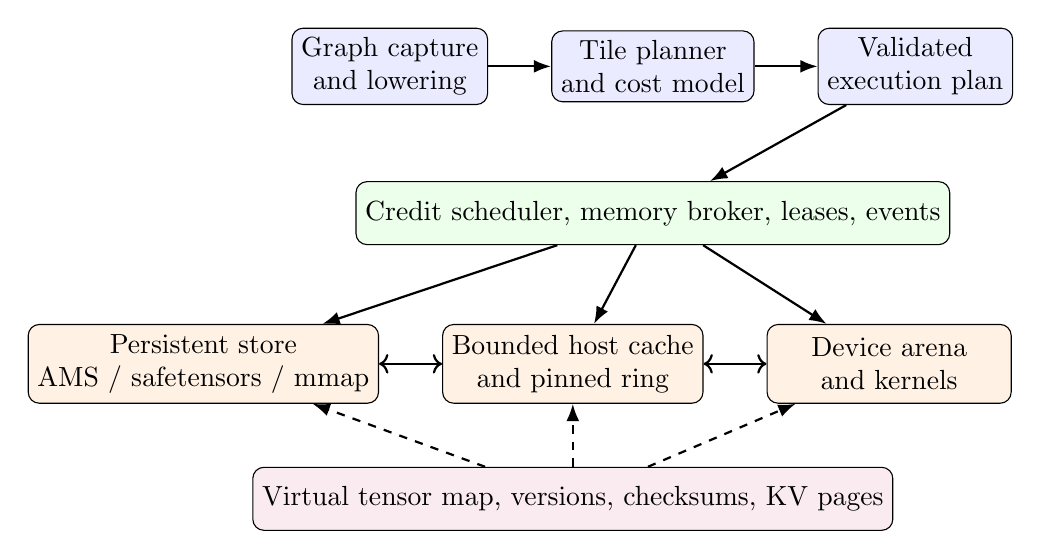
\begin{tikzpicture}[
  node distance=5mm and 8mm,
  box/.style={draw,rounded corners,align=center,minimum height=8mm,minimum width=24mm,fill=white},
  tierbox/.style={draw,rounded corners,align=center,minimum height=10mm,minimum width=31mm},
  arrow/.style={-{Latex[length=2.2mm]},thick}
]
  \node[box,fill=blue!8] (capture) {Graph capture\\and lowering};
  \node[box,fill=blue!8,right=of capture] (planner) {Tile planner\\and cost model};
  \node[box,fill=blue!8,right=of planner] (plan) {Validated\\execution plan};
  \node[box,fill=green!8,below=10mm of planner] (sched) {Credit scheduler, memory broker, leases, events};
  \node[tierbox,fill=orange!10,below left=10mm and -3mm of sched] (store) {Persistent store\\AMS / safetensors / mmap};
  \node[tierbox,fill=orange!10,right=of store] (host) {Bounded host cache\\and pinned ring};
  \node[tierbox,fill=orange!10,right=of host] (device) {Device arena\\and kernels};
  \node[box,fill=purple!8,below=8mm of host] (vt) {Virtual tensor map, versions, checksums, KV pages};
  \draw[arrow] (capture) -- (planner);
  \draw[arrow] (planner) -- (plan);
  \draw[arrow] (plan) -- (sched);
  \draw[arrow] (sched) -- (store);
  \draw[arrow] (sched) -- (host);
  \draw[arrow] (sched) -- (device);
  \draw[arrow,<->] (store) -- (host);
  \draw[arrow,<->] (host) -- (device);
  \draw[arrow,dashed] (vt) -- (store);
  \draw[arrow,dashed] (vt) -- (host);
  \draw[arrow,dashed] (vt) -- (device);
\end{tikzpicture}%
}
\caption{\AMS separates logical tensors and graph semantics from physical residency. The plan fixes bounded resources; the scheduler moves versioned tiles through the hierarchy.}
\label{fig:architecture}
\end{figure}

\section{Executability, Memory Bounds, Progress, and Lower Bounds}
\label{sec:theory}

The central invariant has a simple but important theoretical foundation. Any finite tensor computation can be expanded into a finite scalar computation graph, and finite scalar operations can be evaluated with a bounded fast-memory frontier while values reside in external storage. Practical \AMS plans recover performance by operating on larger tiles and exploiting structure, but the scalar construction establishes a floor beneath all optimized paths.

\subsection{External-memory executability}

\begin{assumption}[Primitive interpreter]
\label{ass:primitive}
There is a backend that can execute every primitive scalar operation in a finite set $\mathcal P$ using at most $\mu_{\mathcal P}$ bytes of fast memory, including operand buffers, result, finite metadata, and bounded workspace. Encoded operands and results can be read from and written to a slower tier.
\end{assumption}

\begin{theorem}[Finite external-memory evaluation]
\label{thm:external-eval}
Let $C$ be a finite, terminating computation whose tensor operators have semantics expressible as a finite acyclic scalar circuit over $\mathcal P$, after unrolling executed finite control flow. If persistent storage holds the circuit inputs and all values selected for spill, transfers and primitives eventually complete, and the fastest tier has capacity at least $R+\mu_{\mathcal P}$ for runtime reserve $R$, then $C$ can be evaluated in finite time with a fastest-tier working set independent of the total bytes of its parameters and intermediate tensors.
\end{theorem}

\begin{proof}
Topologically order the finite scalar circuit. For each scalar node, read its finite operands from persistent storage or a bounded cache, execute the corresponding primitive using the reserved working set, and write the result to a unique spill location. Once all consumers of a spilled value have executed, its location may be reused. At most the runtime reserve, operands of one primitive, its result, and bounded metadata are resident in the fastest tier. The number of nodes and every operation time are finite under the assumptions, so evaluation terminates. The bound depends on primitive arity and representation, not on total parameter bytes. A complete proof including dynamic finite traces appears in Appendix~\ref{app:proofs}.
\end{proof}

\begin{corollary}[Finite LLM request]
\label{cor:llm}
A finite supported LLM request can execute on a local hierarchy when its checkpoint and worst-case spill fit in accessible backing storage and a backend satisfies Assumption~\ref{ass:primitive}. Accelerator memory need not hold the model or any full parameter tensor.
\end{corollary}

The corollary is an existence result, not a throughput result. A scalar plan may perform many tiny reads and writes and can be unusably slow. It nevertheless establishes the fallback that turns ``does not fit in accelerator memory'' into ``has a potentially severe but finite time cost.''

\subsection{Tile-level bounded residency}

Let $P$ be a validated task plan, and let $\mathcal U(t)$ be the set of leases held at time $t$. The broker enforces for every tier $k$,
\[
  \sum_{\ell\in\mathcal U(t)} r_k(\ell) \le C_k-R_k,
\]
where $R_k$ is a non-leasable reserve. External library memory included in the guarantee is charged either as a fixed reserve or as a task workspace.

\begin{theorem}[Managed peak-memory bound]
\label{thm:memory-bound}
Suppose all material allocations in tier $k$ are obtained from a broker whose arena has admitted capacity $C_k-R_k$, every task atomically acquires its declared resource vector before dispatch, and no kernel exceeds its declared workspace. Then managed use of tier $k$ is at most $C_k$ at every time. If all parameter and state tensors are virtual and plans use tiles bounded by constants determined by $C_k$, the bound is independent of total model parameter size.
\end{theorem}

\begin{proof}
The broker invariant bounds the sum of active leases. Arena and alignment overhead are included in the lease sizes or $R_k$. Atomic acquisition prevents a task from holding a partial vector while waiting for the remainder. Since tasks access only leased buffers and kernels obey the workspace contract, no managed allocation can exceed the admitted sum. Virtual tensors map unresident regions to slower tiers, so growing total parameter bytes increases the number of tasks or transfers rather than the size of any admitted buffer.
\end{proof}

\begin{remark}
Sampling \code{cudaMemGetInfo} or an analogous global free-memory value is useful telemetry but does not prove Theorem~\ref{thm:memory-bound}. The value can change between query and allocation; framework allocators may reserve more than tensors currently use; and non-framework allocations may be invisible to framework profilers. The theorem is implemented by ownership and admission, not observation.
\end{remark}

\subsection{Scheduler progress}

The runtime task graph contains storage reads, decode/dequantize steps, transfers, kernels, reductions, and writeback. Resource waits can deadlock if tasks hold one scarce buffer while requesting another. \AMS forbids this pattern.

\begin{assumption}[Eventual service]\label{ass:progress-placeholder}
Every admitted IO, transfer, or compute task eventually completes with success or a terminal error; completion callbacks eventually run; and cancellation eventually quiesces submitted operations.
\end{assumption}

\begin{theorem}[Progress of atomic resource admission]
\label{thm:progress}
Let $D$ be a finite acyclic task graph. Suppose a task is submitted only after all predecessors complete and its complete resource vector is atomically available; a submitted task does not request additional mandatory resources; completed or terminally failed tasks release all leases; and Assumption~\ref{ass:progress-placeholder} holds. If at least one ready task's resource vector fits the configured capacities whenever unfinished work remains, then the scheduler reaches a terminal state without resource deadlock.
\end{theorem}

\begin{proof}
Assume unfinished work remains. Because $D$ is finite and acyclic, some unfinished node has all unfinished predecessors absent; after completed predecessors are removed, at least one node is ready. By hypothesis, at least one ready vector fits. Atomic admission gives that task all mandatory resources, so it cannot participate in hold-and-wait. Eventual service makes it terminal, after which it releases resources and strictly reduces the number of unfinished nodes. Induction proves termination. Fair priority aging prevents starvation among repeatedly fit ready tasks. See Appendix~\ref{app:proofs} for the error and cancellation cases.
\end{proof}

\subsection{Correctness of tiled reductions}

For matrices $X\in\R^{p\times n}$, $W\in\R^{m\times n}$, and $b\in\R^m$, partition row indices $P$, output indices $I$, and reduction indices $J$ into disjoint ordered blocks. Define
\begin{equation}
\label{eq:tiled-linear}
  \widehat Y_{P_a,I_b}
   = b_{I_b}
     +\sum_c X_{P_a,J_c}W_{I_b,J_c}^{\mathsf T}.
\end{equation}

\begin{proposition}[Algebraic correctness of the matrix sweep]
\label{prop:linear-correct}
Over any semiring for which the selected accumulation order is defined, Equation~\eqref{eq:tiled-linear} equals the corresponding block of $XW^{\mathsf T}+\mathbf 1b^{\mathsf T}$. Completed output tiles may be written to and later read from external storage without changing the algebraic result.
\end{proposition}

\begin{proof}
The $c$-th product contributes exactly the terms whose reduction index lies in $J_c$. The blocks form a disjoint cover of the reduction domain, so their sum contains every term exactly once. Output and batch partitioning only selects coordinates. External storage changes residency, not values.
\end{proof}

Attention uses a different associative summary. For a fixed query row and a streamed score/value block, maintain maximum $m$, normalizer $\ell$, and unnormalized weighted value $o$. If a new block has scores $s$ and values $V$, set
\begin{align}
  m' &= \max(m,\max s),\\
  \ell' &= e^{m-m'}\ell + \sum_j e^{s_j-m'},\\
  o' &= e^{m-m'}o + \sum_j e^{s_j-m'}V_j.
\end{align}

\begin{proposition}[Exact online softmax summary]
\label{prop:online-softmax}
In exact real arithmetic, after processing any prefix of score/value blocks, $m$ is the maximum score in the prefix, $\ell=\sum_j e^{s_j-m}$, and $o=\sum_j e^{s_j-m}V_j$. Therefore $o/\ell$ after the final block equals ordinary softmax attention.
\end{proposition}

\begin{proof}
Induct on blocks. Rescaling the old summary by $e^{m-m'}$ expresses all previous exponentials relative to the new maximum; adding the new block establishes the invariant. The base case is the empty summary $m=-\infty$, $\ell=0$, $o=0$. This is the online normalization principle used by IO-aware exact attention algorithms \cite{milakov2018online,dao2022flashattention}.
\end{proof}

\subsection{An unavoidable dense-weight IO floor}

\begin{theorem}[Adversarial read lower bound for exact dense matvec]
\label{thm:dense-lower-bound}
Consider exact computation of $y=Wx$ for an arbitrary dense matrix $W\in\mathbb F^{m\times n}$ over a field and an input $x$ with every coordinate nonzero. Any deterministic algorithm that has no prior information constraining $W$ and must be correct for every $W$ must inspect every matrix entry, or information sufficient to distinguish every entry's value. Thus it consumes $\Omega(mn)$ weight elements from some resident or transferred representation.
\end{theorem}

\begin{proof}
Suppose the algorithm does not inspect information that distinguishes entry $W_{ij}$. Choose matrices $W$ and $W'$ identical in all inspected information and all entries except $W_{ij}\ne W'_{ij}$. The algorithm follows the same execution and returns the same output, but the correct $i$-th outputs differ by $(W_{ij}-W'_{ij})x_j\ne0$, a contradiction.
\end{proof}

The theorem explains the governing time--memory trade. If a dense model is not cached in a faster tier and no exact structure or compression reduces information transfer, the model representation must be consumed during each non-amortized pass. For autoregressive batch-one decode, repeatedly streaming most weights can make per-token time approximately bandwidth-bound by model bytes divided by effective storage/link bandwidth. Batching, caching, sparsity, compression, speculative methods, or keeping hot layers resident can amortize or reduce the traffic, but no scheduler eliminates the adversarial floor.

\subsection{Finite-time upper bound}

Let $N_{\mathrm{tile}}$ be the finite number of tasks, $s_u$ bytes transferred by task $u$, $f_u$ primitive operations, and let every used path have positive effective bandwidth $\underline B$ and every primitive backend positive throughput $\underline F$. Ignoring overlap gives the conservative bound
\[
  T \le \sum_{u=1}^{N_{\mathrm{tile}}}
  \left(\lambda_u+\frac{s_u}{\underline B}+\frac{f_u}{\underline F}\right),
\]
which is finite. A pipelined implementation targets the maximum, rather than the sum, of storage, link, and compute stage times in steady state. The cost model in Section~\ref{sec:planning} turns this observation into plan selection.

\section{Accumulative Matrix Sweeping}
\label{sec:linear}

Dense and quantized linear maps dominate parameter volume in many LLMs. This section defines the reference \AMS operator precisely, including the cases where neither a weight row, the complete input, nor the complete output fits in the compute tier.

\subsection{Logical operation and tiling}

Consider
\[
  Y=XW^{\mathsf T}+\mathbf 1b^{\mathsf T},
  \qquad
  X\in\mathbb F^{p\times n},\quad
  W\in\mathbb F^{m\times n},\quad
  Y\in\mathbb F^{p\times m}.
\]
The leading dimension $p$ may combine batch, sequence, beam, or token groups. Choose ordered partitions
\[
  [0,p)=\bigsqcup_a P_a,
  \qquad [0,m)=\bigsqcup_b I_b,
  \qquad [0,n)=\bigsqcup_c J_c.
\]
For each output tile, initialize
\[
  A_{a,b}\leftarrow \mathbf 1 b_{I_b}^{\mathsf T},
\]
then sweep the reduction blocks:
\begin{equation}
\label{eq:ams-update}
  A_{a,b}\leftarrow A_{a,b}\boxplus
  \operatorname{GEMM}\!
  \left(X_{P_a,J_c},W_{I_b,J_c}^{\mathsf T}\right).
\end{equation}
Here $\boxplus$ is the declared accumulation operation, which may be direct floating addition, pairwise reduction, compensated addition, integer accumulation for quantized kernels, or an exact test semiring. When all $J_c$ are processed, $A_{a,b}$ is committed as $Y_{P_a,I_b}$.

Every logical dimension is therefore virtualizable. If one row of $W$ exceeds fast memory, shrink $J_c$. If the output exceeds fast memory, shrink $P_a$ or $I_b$ and spill completed tiles. If the activation slice exceeds fast memory, shrink $P_a$ or $J_c$. The minimum nontrivial plan can operate on one output scalar and one reduction scalar at a time.

\begin{figure}[H]
\centering
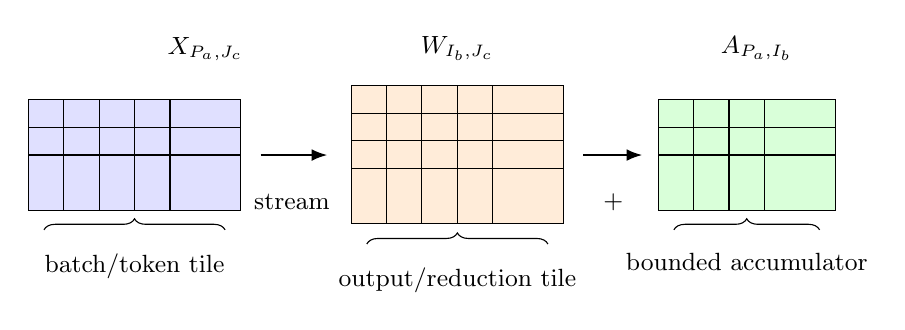
\begin{tikzpicture}[
  cell/.style={draw,minimum width=9mm,minimum height=7mm,inner sep=0pt},
  arr/.style={-{Latex[length=2mm]},thick},
  label/.style={font=\small,align=center}
]
  \node[label] at (0,2.5) {$X_{P_a,J_c}$};
  \foreach \r in {0,...,2}{\foreach \c in {0,...,4}{
    \node[cell,fill=blue!12] at (-1.8+0.45*\c,1.5-0.35*\r) {};
  }}
  \node[label] at (3.2,2.5) {$W_{I_b,J_c}$};
  \foreach \r in {0,...,3}{\foreach \c in {0,...,4}{
    \node[cell,fill=orange!15] at (2.3+0.45*\c,1.68-0.35*\r) {};
  }}
  \node[label] at (7,2.5) {$A_{P_a,I_b}$};
  \foreach \r in {0,...,2}{\foreach \c in {0,...,3}{
    \node[cell,fill=green!15] at (6.2+0.45*\c,1.5-0.35*\r) {};
  }}
  \draw[arr] (0.7,1.15) -- (1.55,1.15);
  \draw[arr] (4.8,1.15) -- (5.55,1.15);
  \node[label] at (1.1,0.55) {stream};
  \node[label] at (5.18,0.55) {$+$};
  \draw[decorate,decoration={brace,amplitude=4pt}] (-2.05,0.2) -- (0.25,0.2)
    node[midway,below=5pt,font=\small] {batch/token tile};
  \draw[decorate,decoration={brace,amplitude=4pt}] (2.05,0.02) -- (4.35,0.02)
    node[midway,below=5pt,font=\small] {output/reduction tile};
  \draw[decorate,decoration={brace,amplitude=4pt}] (5.95,0.2) -- (7.8,0.2)
    node[midway,below=5pt,font=\small] {bounded accumulator};
\end{tikzpicture}
\caption{A true \AMS linear step tiles the output and reduction axes. The accumulator is bounded; it need not be the full output tensor.}
\label{fig:matrix-sweep}
\end{figure}

\subsection{Loop-order families}

The same block equation admits several schedules. The planner selects among them based on reuse, storage layout, and request phase.

\paragraph{Output-stationary sweep.}
For each $(P_a,I_b)$, keep $A_{a,b}$ resident and iterate $J_c$. This minimizes accumulator traffic and is the safest baseline. It may reread $X_{P_a,J_c}$ for each output block.

\paragraph{Input-stationary sweep.}
Keep $X_{P_a,J_c}$ resident while multiplying several $I_b$ blocks. This amortizes activation reads and host-to-device copies, at the cost of several accumulators or repeated output spill. It is attractive for prefill, where $P_a$ is large enough for efficient GEMM.

\paragraph{Weight-stationary reuse.}
Keep $W_{I_b,J_c}$ resident across several token or microbatch tiles. This is valuable in continuous batching and decode, where one weight tile can serve many requests. The scheduler may form a cohort of compatible tokens before evicting the tile.

\paragraph{Layer-stationary or cache-resident path.}
If the complete weight is admitted, choose one tile and call the optimized conventional kernel. The virtual abstraction must not impose per-tile overhead when residency is available.

\paragraph{Split-reduction path.}
Several devices or CPU workers compute disjoint $J_c$ ranges and reduce their partial accumulators. This increases accumulator traffic and changes floating reduction order unless deterministic reduction is selected.

\subsection{Byte-accurate working-set accounting}

A candidate tile is legal only after accounting for storage and compute dtypes, packing, and workspace. For one output-stationary pipeline with $q$ device weight buffers and $h$ host staging buffers,
\begin{align}
M_{\mathrm{device}}
&=R_0+q\,\bytes(W_{I_b,J_c}^{\mathrm{compute}})
 +q_X\bytes(X_{P_a,J_c}^{\mathrm{compute}})
 +\bytes(A_{P_a,I_b}^{\mathrm{acc}}) \notag\\
&\quad +\bytes(b_{I_b})+U_{\mathrm{kernel}}+Z_0,\label{eq:linear-device}\\
M_{\mathrm{pinned}}
&=R_1+h\,\bytes(W_{I_b,J_c}^{\mathrm{storage}})
 +h_X\bytes(X_{P_a,J_c}^{\mathrm{storage}})+Z_1.\label{eq:linear-host}
\end{align}
The planner uses actual dtype sizes and codec expansion. A 4-bit weight tile may require scales, zero points, alignment padding, and a BF16/FP16 or register-level dequantization path. A kernel-selected workspace is included in $U_{\mathrm{kernel}}$. The host ring is bounded; pinning the full checkpoint is neither required nor generally desirable.

\subsection{Bias, residual, and fused epilogues}

Bias is applied exactly once per output coordinate. It may initialize the accumulator or be applied in the final epilogue. Residual addition, activation, scaling, and dropout may be fused only when doing so preserves graph semantics and the output tile is final. Applying a nonlinear activation to partial sums is incorrect:
\[
  \phi\!\left(\sum_c z_c\right)\ne \sum_c\phi(z_c).
\]
in general.
The operator plan marks an accumulator as \code{PARTIAL} until all reduction tiles and required cross-worker reductions finish. Only a \code{FINAL} tile may pass through non-linear epilogues or be consumed by a downstream operator that requires the complete coordinate value.

\subsection{Storage layouts}

A checkpoint stored in ordinary row-major order supports contiguous output-row slices but can make narrow reduction-axis tiles fragmented. A converter should generate one or more tile-major packed layouts selected from an architecture-independent layout family:

\begin{itemize}
  \item row panels $[I_b,0:n)$ for large contiguous layer offload;
  \item two-dimensional panels $[I_b,J_c]$ aligned to filesystem and DMA boundaries;
  \item backend packs for tensor-core or vector kernels, versioned by kernel ABI;
  \item quantized panels containing data and adjacent scale/zero-point metadata;
  \item optional transposed replicas when backward or alternative loop orders justify storage cost.
\end{itemize}

The canonical logical tensor remains layout-independent. Repacking is a conversion/cache operation with hashes linking the packed artifact to the source checkpoint. A portable package must retain or regenerate a generic layout rather than depend solely on a device-specific pack.

\subsection{Asynchronous double or triple buffering}

For buffer depth $q\ge2$, stage $r+1$ can read/decode/copy while stage $r$ computes. Let $H_i$ be pinned host buffers, $D_i$ device weight buffers, and $E_i^{\mathrm{copy}},E_i^{\mathrm{compute}}$ events. A buffer cycle is:

\begin{enumerate}
  \item wait until the prior compute event for slot $i$ has released $D_i$;
  \item fill $H_i$ by asynchronous storage read, or direct-read into $D_i$ when supported;
  \item launch host-to-device copy on a transfer stream and record $E_i^{\mathrm{copy}}$;
  \item make the compute stream wait on $E_i^{\mathrm{copy}}$;
  \item launch the tile kernel and record $E_i^{\mathrm{compute}}$;
  \item reuse $H_i$ only after the copy no longer references it; reuse $D_i$ only after compute completion.
\end{enumerate}

Page-locked host memory is required for genuine asynchronous CPU--GPU copies on CUDA, and overlap depends on hardware copy engines and stream configuration \cite{cuda_async}. The backend capability report determines whether $q=2$, $q=3$, or a serial path is useful.

\subsection{Quantized and compressed weights}

The logical linear operator is independent of storage encoding. A codec plugin declares:
\[
  (d_s,\text{metadata},\text{tile})
  \xrightarrow{\text{decode}}
  W_{I_b,J_c}^{\mathrm{compute}}
\]
and bounds its source bytes, decoded bytes, workspace, alignment, and numeric error. Three implementations are permitted:

\begin{enumerate}
  \item decode into a leased device tile, then call a standard GEMM;
  \item fuse decode into the matrix kernel, avoiding full decoded materialization;
  \item decode on CPU into a bounded pinned buffer when the device lacks support.
\end{enumerate}

Lossless compression preserves exact logical values but may have data-dependent expansion time. Lossy quantization belongs to approximate mode and records calibration, scale conventions, group size, and reference tolerances. The runtime must not reinterpret arbitrary checkpoint bytes based on filename alone.

\subsection{Batched, grouped, and tensor forms}

Linear layers in attention and MoE often have extra logical axes. The operator registry normalizes these to a contraction
\[
  Y_{\alpha,\beta}
   = \sum_{\gamma} X_{\alpha,\gamma}W_{\beta,\gamma}.
\]
After view and batch-index mapping, the registry selects a GEMM, batched GEMM, grouped GEMM, or scalar kernel. A tile descriptor carries logical origins and physical strides; it must not assume contiguous \code{view} is valid. Non-contiguous input views are either materialized into a bounded tile or consumed by a strided kernel.

\subsection{Reference algorithm}

Algorithm~\ref{alg:linear-sweep} gives the semantic baseline. The production scheduler expands the asynchronous calls into task nodes and may reorder independent tiles, but it may not violate accumulator dependencies.

\begin{algorithm}[t]
\caption{Bounded output-stationary linear sweep}
\label{alg:linear-sweep}
\begin{algorithmic}[1]
\Require Virtual tensors $X,W,b,Y$; partitions $\{P_a\},\{I_b\},\{J_c\}$; plan $P$
\ForAll{$P_a$ in request order}
  \ForAll{$I_b$ in planned output order}
    \State $A\gets \Call{LeaseAccumulator}{|P_a|,|I_b|,P.\mathrm{acc\_dtype}}$
    \State $A\gets \Call{BroadcastBiasTile}{b,I_b,A}$
    \ForAll{$J_c$ in declared reduction order}
      \State $X_t\gets \Call{Materialize}{X,(P_a,J_c),P.X\_placement}$
      \State $W_t\gets \Call{Materialize}{W,(I_b,J_c),P.W\_placement}$
      \State $A\gets \Call{MatmulAccumulate}{X_t,W_t,A,P.kernel}$
      \State \Call{ReleaseAfterEvent}{$X_t,W_t$}
    \EndFor
    \State \Call{CommitVirtualTile}{$Y,(P_a,I_b),A$}
    \State \Call{ReleaseAfterEvent}{$A$}
  \EndFor
\EndFor
\end{algorithmic}
\end{algorithm}

\subsection{Planner invariants for linear operators}

Every generated linear plan must satisfy:

\begin{enumerate}
  \item partitions cover each logical domain exactly once and contain no overlap unless an explicit reduction accounts for it;
  \item bias and non-linear epilogues occur once and only after the complete reduction;
  \item all physical byte ranges are bounds-checked and aligned or copied through an alignment buffer;
  \item accumulator type and reduction order match the selected numerical mode;
  \item resource equations, including worst-case codec and kernel workspaces, fit admitted arenas;
  \item every asynchronous source and destination buffer remains leased until its completion event;
  \item an empty dimension, zero-size tile, scalar shape, and tail tile have defined behavior;
  \item output commit is atomic at tile granularity with respect to downstream consumers.
\end{enumerate}

\section{Stream-Decomposable LLM Operator Catalog}
\label{sec:operators}

A universal model-level invariant cannot stop at linear layers. This section specifies reference stream plans for the operator families required by contemporary language models. The optimized implementation may fuse or replace them, but every supported graph must lower to semantics equivalent to these plans.

\subsection{Embeddings and tied output projections}

For token indices $t_1,\ldots,t_p$ and embedding table $E\in\mathbb F^{V\times d}$, gather only requested rows. The planner sorts or groups repeated indices for coalesced reads, then restores request order. A bounded tile can contain one row; therefore vocabulary size does not enter fast-memory capacity. Position embeddings, segment embeddings, and learned scaling are pointwise additions on tiles.

Tied input/output embeddings share a \code{storage\_id}. The language-model head is a linear contraction against the same logical tensor, possibly through a transposed packed view. The converter must not materialize a duplicate merely because framework state dictionaries expose aliases differently.

\subsection{Layer normalization and RMS normalization}

For a vector $x\in\mathbb F^d$, layer normalization requires mean and variance. A stable two-pass plan is:
\begin{align}
  \mu &= \frac1d\sum_j x_j,\\
  q &= \sum_j (x_j-\mu)^2,\\
  y_j &= \gamma_j\frac{x_j-\mu}{\sqrt{q/d+\epsilon}}+\beta_j.
\end{align}
A one-pass Welford summary may reduce reads while retaining numerical stability. The summary state $(n,\mu,M_2)$ is constant-size and mergeable across tiles. RMS normalization maintains $q=\sum_j x_j^2$ and applies scale in a second pass. Inputs may be reread from storage, retained when they fit, or rematerialized from a preceding operator. The planner chooses based on IO cost.

Residual addition, scalar multiplication, clipping, RoPE, masks, and elementwise activations are coordinate-wise and tile trivially. A fused residual-plus-normalization plan must preserve whether the residual is consumed elsewhere and whether the normalized output is computed from pre- or post-residual values.

\subsection{Feed-forward and gated MLP blocks}

A standard feed-forward block
\[
  Z=\phi(XW_1^{\mathsf T}+b_1),\qquad
  Y=ZW_2^{\mathsf T}+b_2
\]
can spill $Z$ by token and hidden tiles. A more efficient plan fuses an intermediate tile: compute a final $Z_{P,H_c}$ tile, apply $\phi$, then immediately sweep it into partial output accumulators for $W_2[:,H_c]$. This avoids materializing the complete expanded hidden activation but may require several output accumulators or repeated $Z$ computation.

For SwiGLU or another gated block,
\[
  Z=\operatorname{silu}(XW_g^{\mathsf T})\odot(XW_u^{\mathsf T}),
  \qquad Y=ZW_d^{\mathsf T},
\]
the gate and up-projection tiles for the same intermediate coordinates must be final before multiplication. The resulting $Z$ tile can then be consumed by the down projection. The planner may co-pack corresponding rows of $W_g$ and $W_u$ to reduce storage seeks.

Three schedules are required:

\begin{enumerate}
  \item \emph{materialize-intermediate}: simplest and best when host/storage bandwidth is high and accumulator memory is low;
  \item \emph{fused-intermediate}: retain one $Z$ tile and update one or more output accumulators;
  \item \emph{recompute-intermediate}: reproduce a $Z$ tile for each output block, trading compute and repeated first-layer weight reads for less accumulator storage.
\end{enumerate}

The cost model must include all three; there is no universally optimal choice.

\subsection{Exact streamed attention}

Let query block $Q\in\mathbb F^{q\times d_h}$ attend to key/value blocks $K_r,V_r$ with scores
\[
  S_r=QK_r^{\mathsf T}/\sqrt{d_h}+M_r.
\]
For each query row, maintain $(m,\ell,O)$ as in Proposition~\ref{prop:online-softmax}. The block update is
\begin{align}
  m' &= \max\left(m,\operatorname{rowmax}(S_r)\right),\\
  P_r &= \exp(S_r-m'\mathbf 1^{\mathsf T}),\\
  \alpha &= \exp(m-m'),\\
  \ell' &= \alpha\odot\ell+P_r\mathbf 1,\\
  O' &= \operatorname{diag}(\alpha)O+P_rV_r.
\end{align}
After the final block, return $O/\ell$. Causal, sliding-window, prefix, and block-sparse masks are represented by $M_r$ or by skipping blocks known to be all masked. The score matrix is a bounded scratch tile and is never required in full.

The implementation should reuse FlashAttention-class kernels when Q, K, and V subproblems fit; the external-memory layer wraps those kernels and pages K/V blocks from lower tiers. Exactness refers to the mathematical softmax; floating behavior follows Section~\ref{sec:numerics}.

\subsection{Virtual KV cache}

KV state is a virtual tensor indexed by request, layer, head/group, token position, and head dimension. Physical pages have fixed byte classes and independent tier placement. Required operations are:

\begin{itemize}
  \item append K/V rows transactionally after a token step;
  \item gather an ordered logical range into attention blocks;
  \item share immutable prefix pages across requests;
  \item copy-on-write the final partially filled page;
  \item evict cold pages to host or storage and prefetch predicted next blocks;
  \item release all request-owned pages on completion or cancellation;
  \item compact or remap without changing logical addresses.
\end{itemize}

PagedAttention shows the value of virtual paging for KV cache \cite{kwon2023pagedattention}. \AMS generalizes the page manager so KV pages, activation spill, and parameter tiles use one resource and integrity model while retaining operator-specific layouts.

For a context too large even for host memory, attention streams KV pages from persistent storage. This preserves capacity but can impose $O(L)$ storage traffic per generated token for dense full-context attention. Sliding-window, recurrent compression, KV quantization, or rematerialization may reduce traffic in approximate or architecture-specific modes, but the baseline remains exact.

\subsection{Vocabulary projection, softmax, \texorpdfstring{top-$k$}{top-k}, and sampling}

A vocabulary projection may produce a logits vector larger than fast memory. The operator uses output tiles of the LM head and either spills logits or feeds them into an online consumer.

For exact softmax probabilities, use two passes or a mergeable summary:
\[
  m=\max_i z_i,
  \qquad \ell=\sum_i e^{z_i-m}.
\]
A second pass emits normalized probabilities by tile. For greedy decoding, only the global argmax pair $(z_i,i)$ is needed. For top-$k$, maintain a bounded heap of $k$ candidates while streaming. For top-$p$, exact selection generally requires enough distribution information to identify the cumulative cutoff; implementations may spill sorted runs and perform an external merge, or keep all logits in a slower tier. Approximate top-$p$ must be explicitly declared.

Sampling must be reproducible under deterministic mode. The random draw is associated with a request token ordinal, not task completion order. Counter-based RNG lets tile scheduling change without changing the random variate. A stable sampling algorithm uses the same logical probability order regardless of physical tile order.

\subsection{Mixture-of-experts}

An MoE layer contains a router and expert networks. The reference plan is:

\begin{enumerate}
  \item compute router logits in tiles and select exact top-$k$ experts per token;
  \item form a bounded dispatch table, spilling it if necessary;
  \item group tokens by expert and capacity slot;
  \item for each expert with assigned tokens, stream its MLP weights and execute the gated or standard MLP plan;
  \item accumulate weighted expert outputs into token output tiles;
  \item apply declared overflow, capacity, and normalization semantics.
\end{enumerate}

Sparse activation can reduce transferred weights because inactive experts need not be read, but the guarantee cannot assume a favorable routing distribution. A worst-case spill estimate includes all routed tokens and configured expert capacity. Popular sparse architectures such as Switch Transformers \cite{fedus2021switch} and Mixtral \cite{jiang2024mixtral} fit this contract when their routing semantics are represented in the operator attributes.

\subsection{Convolutions}

A convolution output tile depends on an input tile enlarged by the kernel halo. The planner tiles batch, output channel, spatial axes, and input-channel reduction. For each output tile, it initializes a bounded accumulator and sweeps input-channel and kernel tiles. Padding is generated logically and need not be stored. Direct, im2col, Winograd, or FFT kernels may be used when their complete workspace is declared. The scalar fallback enumerates output coordinates and kernel support.

Depthwise and grouped convolutions expose independent groups and often have smaller minimum working sets. Transposed convolution requires scatter accumulation; the plan partitions output ownership or uses deterministic reduction buffers to avoid uncontrolled atomic workspaces.

\subsection{State-space and recurrent operators}

For a recurrence
\[
  h_t=F_t(h_{t-1},x_t),\qquad y_t=G_t(h_t,x_t),
\]
the carry $h_t$ is the bounded sequential summary when its state dimension fits. If the state vector itself does not fit, tile the state dimension when $F_t$ is separable or has a registered block algorithm; otherwise invoke the scalar interpreter. Selective state-space models such as Mamba use hardware-aware scan algorithms \cite{gu2023mamba}; \AMS registers both optimized chunked-scan plans and a recurrent fallback. The operator definition must specify whether cross-state coupling requires a reduction or matrix sweep at each time step.

Parallel scan plans associate each sequence block with a summary transform and combine summaries in a tree. The planner may prefer recurrent execution for decode and parallel scan for prefill. Mutable recurrent state is versioned per request and checkpointed only according to session policy.

\subsection{Collectives and reductions}

Sum, max, min, logical reductions, norms, and histograms use mergeable summaries. A reduction plan declares associativity assumptions, identity, accumulator dtype, and deterministic merge order. Non-associative custom reductions must specify an order-preserving stream implementation or are unsupported in strict mode.

Cross-device collectives are represented as tasks with declared communication buffers. Their library workspaces and communicator allocations are reserved during backend initialization; they may not appear as hidden allocations during a guaranteed request.

\subsection{Views, slicing, concatenation, and indexing}

Reshape and transpose are metadata-only when the requested tile remains representable as bounded physical spans. Otherwise, a bounded retiling copy materializes the target layout. Concatenation creates a logical segmented view; downstream tile reads are split at segment boundaries. Slice is a view. Gather and scatter use bounded index blocks, validate indices before physical access, and define duplicate-index accumulation order.

\subsection{Operator coverage table}
Table~\ref{tab:operators} records the required bounded-state decomposition and its principal hazards for each operator family.

\begin{table}[p]
\centering
\caption{Reference stream state and principal tiled axes. ``Finalization'' identifies the point before a non-linear consumer may observe a tile.}
\label{tab:operators}
\small
\begin{tabularx}{\textwidth}{@{}p{0.16\textwidth}p{0.22\textwidth}p{0.25\textwidth}X@{}}
\toprule
Operator & Principal tile axes & Bounded persistent summary & Finalization condition \\
\midrule
Linear / projection & tokens, output, reduction & output accumulator & all reduction blocks complete \\
Embedding gather & requested rows, feature & deduplication/index map & requested row materialized \\
LayerNorm & tokens, feature & Welford or $(\sum x,\sum x^2)$ & statistics complete; second pass applied \\
RMSNorm & tokens, feature & sum of squares & norm complete; scale applied \\
MLP / SwiGLU & token, intermediate, output & intermediate tile and/or output accumulators & both gated projections and down reduction complete \\
Attention & query, KV block, head & online $(m,\ell,O)$ & all visible KV blocks complete \\
KV append & request, layer, page & page table and partial page & page data and table update committed \\
LM head & token, vocabulary, reduction & logits tile or online selection summary & hidden reduction complete \\
Softmax & vocabulary block & $(m,\ell)$ & max/sum complete and output pass done \\
Top-$k$ & vocabulary block & size-$k$ heap & all logits inspected \\
Top-$p$ & vocabulary runs & external sorted runs / distribution state & cumulative cutoff proven \\
MoE & token, expert, hidden & route table and token output accumulators & all selected expert contributions complete \\
Convolution & batch, channel, spatial, kernel & output accumulator and halo tile & all input-channel/kernel blocks complete \\
SSM / recurrence & time, state block & carry or block-transform summary & predecessor carry / scan prefix complete \\
Elementwise & any coordinate axes & none beyond tile & local tile computed \\
\bottomrule
\end{tabularx}
\end{table}

\subsection{Custom operator contract}

A custom operator is admissible only if its plugin supplies:

\begin{enumerate}
  \item a pure logical semantic function or test oracle;
  \item shape, dtype, alias, mutation, and numerical-mode rules;
  \item \code{minimum\_working\_set(capabilities, shape)};
  \item one or more plan generators with complete resource declarations;
  \item kernel implementations or a decomposition into registered primitives;
  \item backward and saved-state rules if training is supported;
  \item differential, property, bounds, cancellation, and corruption tests;
  \item a versioned ABI and security classification.
\end{enumerate}

Opaque plugins that allocate through global device allocators, launch untracked asynchronous work, or retain pointers beyond leases are excluded from Level II guarantees.

\section{Resource-Aware Planning and Cost Modeling}
\label{sec:planning}

The planner converts a functional logical graph and a request envelope into a finite task template whose resource bounds are admissible and whose estimated cost is minimal among considered legal plans. Correctness and fit are hard constraints; performance is the objective.

\subsection{Planner inputs}

The planner receives:

\begin{itemize}
  \item graph IR, symbolic shapes, alias sets, and operator semantics;
  \item checkpoint manifest, physical layouts, codecs, and storage topology;
  \item backend capabilities, supported kernels, dtype rules, and workspace bounds;
  \item calibrated transfer and compute models;
  \item per-tier reservations, concurrency limits, and tenant quotas;
  \item request envelope: batch/token bounds, context bound, beam/speculation policy, and generation horizon;
  \item numerical, determinism, reliability, latency, throughput, and energy policy;
  \item cache state or a conservative cold-cache assumption.
\end{itemize}

The output is a plan as defined in Section~\ref{sec:model}, plus a structured explanation of rejected alternatives.

\subsection{Preflight and reservations}

Preflight proceeds from slowest to fastest constraints:

\begin{enumerate}
  \item validate manifest, model/operator compatibility, finite shape bounds, and storage byte ranges;
  \item calculate checkpoint, session-state, worst-case KV, activation spill, training state, journal, and temporary conversion requirements;
  \item choose candidate backends and reserve fixed runtime bases, including library contexts and communicators;
  \item request a device/DRAM arena under configured quotas rather than consuming all observed free memory;
  \item generate a minimum-working-set plan for every operator; if a device plan fails, shrink tile classes and then try the next backend;
  \item solve or heuristically select a graph plan and validate aggregate liveness and spill;
  \item preallocate or hard-limit arenas and issue an immutable reservation token;
  \item dry-run metadata-only task expansion and verify every resource vector against the token.
\end{enumerate}

Global free-memory telemetry may inform the amount requested, but the accepted amount is the reservation actually obtained. The runtime keeps a safety margin for driver state, display usage, framework internals, and explicitly identified external consumers.

\subsection{Per-tile cost model}

For a task or pipeline stage $u$, define
\begin{align}
T_{\mathrm{storage}}(u)&=\lambda_s(n_u,s_u)+\frac{s_u}{B_s(s_u,n_u)},\\
T_{\mathrm{link}}(u)&=\lambda_p(c_u,s'_u)+\frac{s'_u}{B_p(s'_u,c_u)},\\
T_{\mathrm{compute}}(u)&=\lambda_k(k_u)+\frac{f_u}{F_k(\text{shape},d,\text{layout})},
\end{align}
where $n_u$ is read count, $s_u$ storage bytes, $c_u$ copy count, $s'_u$ link bytes, $f_u$ operations, and all rates are empirically calibrated. Decode/dequantization CPU time, output spill, and synchronization are separate terms.

For a stable $q$-stage overlapped pipeline, a first-order estimate is
\begin{equation}
\label{eq:pipeline-cost}
T(P)\approx T_{\mathrm{fill}}+T_{\mathrm{drain}}
 +N\max(T_{\mathrm{storage}},T_{\mathrm{decode}},T_{\mathrm{link}},T_{\mathrm{compute}})
 +T_{\mathrm{contention}}.
\end{equation}
When the backend cannot overlap stages, the model uses the appropriate sum. Calibration stores confidence intervals and falls back to conservative upper estimates when a size/layout pair is unmeasured.

\subsection{IO and reuse accounting}

The planner counts physical bytes, not logical tensor bytes. It includes alignment, filesystem blocks, codec metadata, page-cache behavior, and repeated reads induced by loop order. For an output-stationary linear plan,
\[
  Q_W=\sum_{a,b,c}\bytes(W_{I_b,J_c}).
\]
After cache reuse; an input-stationary plan may reduce $Q_X$ at the cost of output spill. The model estimates:

\begin{itemize}
  \item checkpoint reads by tier and read-size distribution;
  \item host-to-device and device-to-host bytes;
  \item accumulator and activation spill/readback;
  \item KV page reads per token;
  \item cache hit probability for hot tiles;
  \item decompression and repacking bytes;
  \item write amplification and durability costs in training.
\end{itemize}

Small random reads are penalized because persistent storage often delivers lower effective bandwidth than large contiguous reads. Tile-major packing and row/column bundling follow the same hardware-aware principle explored by LLM in a Flash \cite{alizadeh2023llmflash}.

\subsection{Candidate generation}

Each operator plugin provides a finite candidate family rather than an unbounded integer search. For a linear operator, candidate dimensions derive from:

\begin{itemize}
  \item backend kernel multiples and maximum dimensions;
  \item powers of two and storage-page/alignment boundaries;
  \item full logical dimensions when they fit;
  \item measured sweet spots for GEMM and transfer sizes;
  \item a guaranteed descending chain ending at the minimum working set.
\end{itemize}

For every tile tuple, the plugin enumerates legal loop orders, buffer depth, layouts, accumulator modes, fusion choices, and placement paths. It rejects resource-infeasible candidates before cost evaluation. Tail behavior is explicitly modeled rather than assumed negligible.

\subsection{Graph-level liveness and fusion}

Operator-local minima can be globally poor. The graph planner computes liveness intervals for virtual values and identifies tile pipelines that avoid external materialization. Examples include:

\begin{itemize}
  \item Q/K/V projection tiles feeding attention without complete Q, K, or V materialization;
  \item gated MLP intermediate tiles feeding the down projection;
  \item residual-add plus normalization with a shared input tile;
  \item LM-head logits feeding top-$k$ without storing the vocabulary vector;
  \item KV projection tiles appended directly into cache pages.
\end{itemize}

Fusion is represented as a compound plan with one resource proof. It may be disabled for debugging, deterministic order, backend limitations, or because it increases rereads. The compiler never fuses across mutation, alias, numerical, or control-flow barriers without an equivalence rule.

\subsection{Optimization formulation}

A complete optimizer can formulate plan selection as a mixed-integer program similar in spirit to heterogeneous placement optimization in FlexGen \cite{sheng2023flexgen}. A production default should use a faster staged heuristic:

\begin{enumerate}
  \item select legal per-operator candidates on the Pareto frontier of time, device bytes, host bytes, and spill bytes;
  \item apply graph rewrite templates and recompute frontiers;
  \item run beam search or dynamic programming over block/layer boundaries with bounded frontier size;
  \item reserve a global KV and request-state budget;
  \item simulate task liveness and reject any plan that violates the exact broker model;
  \item locally tune tile sizes using calibration data;
  \item retain the safest candidate and at least one smaller fallback.
\end{enumerate}

The optimization objective may be
\[
  \min_P\; w_L T_{p99}(P)+w_T/T_{\mathrm{throughput}}(P)
  +w_EE(P)+w_WQ_{\mathrm{write}}(P),
\]
subject to hard capacities, numeric semantics, and service-level constraints. Weights are policy, not embedded constants.

\subsection{Prefill and decode plans}

Prefill has many token rows and often achieves high GEMM efficiency; decode has few rows and is weight-bandwidth dominated. A single plan is therefore rarely optimal.

The prefill plan favors large token tiles, batched attention blocks, and activation reuse. The decode plan favors weight caching, request cohorting, grouped GEMV/GEMM, and low-latency priorities. The runtime may switch plans at a token boundary after all mutable tiles are committed. Prompt chunks can use a sequence of shape-specialized plans.

\subsection{Adaptive pressure and replanning}

Within a valid reservation, cache occupancy can change freely. Changing arena capacity or tile shape requires a safe-point replan:

\begin{enumerate}
  \item stop admitting tasks that cross the designated boundary;
  \item let in-flight tasks finish or cancel them according to idempotence policy;
  \item commit dirty state and release plan-specific leases;
  \item obtain a new reservation and validate a smaller or alternate plan;
  \item resume from the last committed virtual-tensor versions.
\end{enumerate}

A sudden external memory-pressure signal may trigger cache eviction immediately, but it cannot justify breaking active leases. If a cooperative platform revokes reserved capacity, the runtime returns \code{RESERVATION\_LOST} or migrates at a safe point; it does not recursively catch OOM inside arbitrary kernels and hope that a smaller tile is semantically restartable.

\subsection{Plan cache and reproducibility}

A plan-cache key includes model content hash, graph hash, operator-plugin versions, backend and driver fingerprint, device topology, storage identity, calibrated profile version, request envelope, and numerical policy. Cached plans are revalidated against current reservations and file hashes. The plan and calibration snapshot are attached to traces so a performance or numerical incident can be replayed.

\subsection{Planner acceptance properties}

Before release, property tests must establish that for random legal shapes and budgets:

\begin{itemize}
  \item candidate generation always reaches a minimum-working-set candidate when preconditions hold;
  \item no accepted resource vector exceeds its tier budget;
  \item partition covers and reduction dependencies are complete;
  \item smaller budgets never force an undeclared approximation;
  \item cost estimates use physical byte ranges and bounded workspaces;
  \item the selected plan is no worse than the explicitly retained safe fallback under the same model;
  \item serialization and deserialization preserve all proof-relevant fields.
\end{itemize}

\section{Runtime Architecture and Asynchronous Data Path}
\label{sec:runtime}

The runtime realizes a validated plan without allowing implementation details to escape its memory proof. This requires explicit ownership of buffers, task dependencies, storage requests, kernel workspaces, and state versions.

\subsection{Core components}

The reference architecture contains the following independently testable components.

\begin{description}[style=nextline]
  \item[\code{ExecutionEngine}] Owns session lifecycle, plan validation, request admission, safe points, cancellation, and terminal status.
  \item[\code{MemoryBroker}] Owns per-tier arenas, resource credits, leases, epochs, reserves, fragmentation accounting, and high-water telemetry.
  \item[\code{VirtualTensorManager}] Resolves logical tiles to physical regions, versions, aliases, replicas, codecs, and integrity metadata.
  \item[\code{TensorStore}] Provides asynchronous bounded reads/writes, range validation, cache hints, atomic commit, and backend-specific direct paths.
  \item[\code{TransferEngine}] Moves tiles between tiers, owns copy streams/queues and events, and exposes overlap capabilities.
  \item[\code{TaskScheduler}] Maintains dependency-ready queues, atomically admits resource vectors, applies priorities and aging, and processes completions.
  \item[\code{Backend}] Provides kernels, streams/queues, events, fixed workspace algorithms, device telemetry, and deterministic capability declarations.
  \item[\code{KVManager}] Allocates logical KV pages, sharing and copy-on-write, eviction, prefetch, and request cleanup.
  \item[\code{PlanExecutor}] Instantiates operator task templates for concrete tile coordinates and binds leases to kernel arguments.
  \item[\code{Telemetry}] Emits traces, counters, structured logs, plan IDs, byte accounting, cache state, numeric diagnostics, and fault records.
\end{description}

Public APIs depend on interfaces, not concrete CUDA or Linux classes. Backend implementations may use Python for orchestration and C++, Rust, CUDA, HIP, Metal, or SYCL for critical paths, but the ownership model is uniform.

\subsection{Memory broker and arenas}

For each guaranteed tier, the broker initializes one or more arenas with size classes aligned to common tile buffers. Device arenas should be created after backend contexts and fixed library reserves so their capacity reflects those costs. Host pinned arenas are intentionally small rings; pageable cache and spill have separate quotas.

A \emph{lease} contains arena, offset, size, alignment, access mode, owner task, epoch, and terminal event. It is move-only in native code and cannot outlive its arena. Views borrow from a lease and cannot be stored in long-lived plugin state. Debug builds poison recycled buffers and validate epochs to detect use-after-release.

Fragmentation is bounded by design. Candidate tile sizes map to a finite set of size classes, and the planner charges class-rounded bytes. Large persistent allocations use dedicated segments. Coalescing allocators may be provided for irregular CPU spill, but the device guarantee must not depend on a best-effort global caching allocator.

\subsection{Atomic admission}

A task descriptor contains its complete resource vector. The scheduler calls
\[
  \operatorname{try\_lease}(\mathbf r(u))
\]
under one broker transaction. Success returns all leases; failure returns none. The task remains ready and is reconsidered when relevant credits are released. This no-partial-hold rule establishes the progress theorem and makes backpressure explicit.

Some resources are capacities rather than memory: number of asynchronous reads, copy-stream slots, compute queues, decompressor workers, file descriptors, and journal transactions. They are credits in the same vector, preventing a task from occupying memory while waiting indefinitely for an unbounded external queue.

\subsection{Task graph}

A materialized operator tile expands to typed tasks such as
\[
\begin{aligned}
\textsc{Read}&\to\textsc{Verify}\to\textsc{Decode}\to\textsc{Copy}\\
&\to\textsc{Compute}\to\textsc{Reduce}\to\textsc{Commit}\to\textsc{Evict}.
\end{aligned}
\]
Tasks are idempotent or explicitly non-idempotent. Immutable reads, verification, decode, and pure compute are retryable. A mutable commit uses a transaction ID and exactly-once version rule. The executor never repeats a non-idempotent task after an ambiguous failure without consulting the journal.

Each edge may carry an event and a virtual-tensor version rather than a host synchronization. Device compute waits on transfer events; downstream device kernels wait on compute events; host callbacks only update scheduler state after events signal. Blocking synchronization is reserved for safe points, debugging, or backends that lack asynchronous primitives.

\subsection{Asynchronous pipeline}
Figure~\ref{fig:pipeline} shows the steady-state overlap pattern used only when the selected storage and backend capabilities permit it.

\begin{figure}[H]
\centering
\resizebox{\linewidth}{!}{%
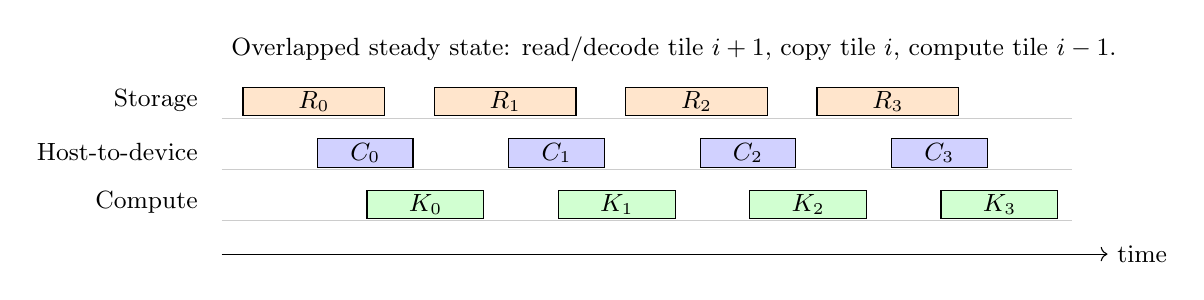
\begin{tikzpicture}[x=0.9cm,y=0.65cm,font=\small]
  \draw[->] (0,0) -- (12.5,0) node[right] {time};
  \foreach \y/\name in {3/Storage,2/Host-to-device,1/Compute}{
    \node[anchor=east] at (-0.2,\y) {\name};
    \draw[gray!40] (0,\y-0.35) -- (12,\y-0.35);
  }
  \foreach \i in {0,...,3}{
    \pgfmathsetmacro{\x}{0.3+2.7*\i}
    \draw[fill=orange!20] (\x,2.7) rectangle ++(2.0,0.55)
      node[midway] {$R_{\i}$};
    \draw[fill=blue!18] (\x+1.05,1.7) rectangle ++(1.35,0.55)
      node[midway] {$C_{\i}$};
    \draw[fill=green!18] (\x+1.75,0.7) rectangle ++(1.65,0.55)
      node[midway] {$K_{\i}$};
  }
  \node[align=left,anchor=west] at (0,4.0) {Overlapped steady state: read/decode tile $i+1$, copy tile $i$, compute tile $i-1$.};
\end{tikzpicture}%
}
\caption{Illustrative three-stage tile pipeline. Actual overlap is capability- and contention-dependent; event lifetimes retain every source and destination buffer.}
\label{fig:pipeline}
\end{figure}

On Linux, storage adapters may use \code{io\_uring}, asynchronous pread, memory mapping, or a direct-IO path. Windows and macOS use platform-native equivalents. Direct storage-to-device DMA such as GPUDirect Storage may bypass the pinned ring where supported \cite{nvidia_gds}; the portable path is storage to bounded host buffers to the device. The API exposes a task, not a specific syscall, so the planner can cost each path.

A pipeline slot is a compound lease. Slot reuse waits for the latest event touching each constituent buffer. Read cancellation does not immediately free a buffer if the OS or DMA engine can still write to it. Backends must provide a quiescence primitive used during cancellation and shutdown.

\subsection{Scheduling policy}

Ready tasks are partitioned into priority classes:

\begin{enumerate}
  \item latency-critical decode tasks on the active token frontier;
  \item tasks that unblock scarce buffers or complete a reduction;
  \item prefetch tasks on the predicted critical path;
  \item prefill and throughput batch tasks;
  \item cache population, repacking, verification, and maintenance.
\end{enumerate}

Within a class, the scheduler uses critical-path estimate, deadline slack, locality benefit, and age. Aging prevents starvation. Resource-aware selection prefers a set of tasks whose vectors fit without fragmenting size classes, but it cannot reorder a deterministic reduction beyond its declared merge tree.

A request can be assigned a weighted fair-share budget. Multi-tenant mode isolates device credits, host cache, pinned buffers, IO depth, and spill quota; it does not merely prioritize queues while allowing one tenant to occupy all memory.

\subsection{Caching and eviction}

Caches are optional performance layers above virtual storage. Entries are immutable parameter tiles, decoded packs, activation checkpoints, or clean KV pages. Cache keys include content version, logical tile, physical layout, dtype/codec, backend pack version, and numerical mode.

Eviction uses cost-aware recency:
\[
  \operatorname{value}(e)
  =\frac{p_{\mathrm{reuse}}(e)\cdot t_{\mathrm{reload}}(e)
  +t_{\mathrm{recompute}}(e)}{\bytes(e)}.
\]
This score is applied after mandatory pin and dirty-state rules. Decode-critical weights may be protected; large one-use prefill tiles are evicted quickly. The cache consumes broker credits and can be shrunk to zero without invalidating correctness.

Dirty mutable tiles follow writeback or write-through policy. Inference KV pages may be dropped if they can be rematerialized under policy, but ordinary exact mode writes them to the selected lower tier before eviction. Training parameters and optimizer state require transactional writeback.

\subsection{Storage layer}

\code{TensorStore} is a logical interface with adapters for:

\begin{itemize}
  \item read-only safetensors and sharded safetensors;
  \item memory-mapped native checkpoint ranges;
  \item the AMS packed container in Appendix~\ref{app:formats};
  \item local filesystem buffered and direct IO;
  \item optional TensorStore/Zarr-style chunked arrays \cite{tensorstore};
  \item optional direct device IO;
  \item testing stores that inject delay, short reads, corruption, and failure.
\end{itemize}

A read request specifies storage object, byte ranges, destination capability, expected checksum, priority, deadline class, and cancellation token. The adapter may coalesce adjacent ranges but must preserve the mapping to logical tiles. It validates every offset and length with overflow-safe arithmetic before issuing IO.

The checkpoint is never deserialized through executable pickle in the trusted default path. Safetensors-style metadata and explicit tensor bytes are preferred \cite{safetensors}. PyTorch checkpoints may be imported in a conversion sandbox using metadata-only and memory-mapped loading where available \cite{pytorch_serialization}.

\subsection{Backend abstraction}

A backend capability record includes:

\begin{itemize}
  \item device kind, count, topology, memory capacities, and allocation alignment;
  \item supported storage/compute dtypes and conversions;
  \item kernel catalog, shape constraints, deterministic variants, and workspace bounds;
  \item streams/queues, event semantics, asynchronous copy paths, and copy-engine counts;
  \item peer access and collective support;
  \item direct storage capability;
  \item timer resolution and profiling support;
  \item minimum scalar or vector fallback.
\end{itemize}

The core implementation should support a CPU backend first because it is the universal semantic reference. CUDA, ROCm/HIP, Metal/MPS, XPU/SYCL, Vulkan, or other backends are plugins. ``Hardware agnostic'' means that the graph and virtual tensor contracts are portable and every supported backend has a safe fallback; it does not mean that one kernel binary or identical tile shape is optimal everywhere.

\subsection{Fault handling and recovery}

Every terminal error propagates through dependent tasks, which are cancelled before admission. Already submitted tasks are quiesced; their leases remain valid until events finish. Immutable corrupted reads are retried from another replica when available. Repeated checksum mismatch marks the storage object unhealthy and terminates with evidence.

Mutable commits use:

\begin{enumerate}
  \item write new tile bytes to a temporary region;
  \item flush according to durability policy;
  \item record checksum and target logical version in a write-ahead journal;
  \item atomically publish the region map update;
  \item retire the old version after readers release it;
  \item truncate or checkpoint the journal.
\end{enumerate}

Inference without durable sessions can choose a lighter policy. Training checkpoints must use a crash-consistent policy and record RNG, optimizer, scaler, and scheduler state.

\subsection{Observability}

Every request trace records plan ID and, subject to cardinality controls:

\begin{itemize}
  \item current and peak leases by tier, class, and owner;
  \item logical and physical bytes read/written by path;
  \item read-size histogram, queue depth, bandwidth, and latency;
  \item host/device copy overlap and idle gaps;
  \item kernel time, workspace, tile shapes, and achieved arithmetic rate;
  \item cache hits, evictions, prefetch usefulness, and recomputations;
  \item scheduler ready/wait times and resource-blocking reasons;
  \item KV page residency and spill;
  \item numerical diagnostics and deterministic-mode identifiers;
  \item retries, integrity failures, replans, cancellations, and cleanup time.
\end{itemize}

Metrics expose OpenTelemetry/Prometheus-compatible instruments, while a binary trace preserves high-rate task events. Tensor contents are not logged by default. A plan simulator consumes traces to compare predicted and actual stage costs.

\section{Automated Graph Transformation and Compiler Integration}
\label{sec:compiler}

Replacing instances of \code{nn.Linear} is not a sufficient graph transformation. Real model code uses functional operators, fused projections, tensor views, tied storage, custom kernels, dynamic control flow, and operations in which a parameter is read without calling its owning module. \AMS therefore compiles a functional graph into a virtual-tensor task program; module replacement is only a compatibility front end.

\subsection{Front-end pipeline}

For PyTorch, the preferred pipeline is:

\begin{enumerate}
  \item instantiate the model skeleton on a metadata device or import an exported graph without materializing parameters;
  \item capture a sound graph with \code{torch.export} under explicit dynamic-shape constraints;
  \item functionalize mutation and aliasing and apply selected decompositions to a stable ATen-level operator set;
  \item lift parameters, buffers, constants, and state into explicit graph inputs or state objects;
  \item propagate symbolic shapes, dtypes, layouts, and alias sets using fake/meta tensors;
  \item canonicalize composite patterns into \AMS semantic operators;
  \item lower each operator through the registry, perform liveness/fusion analysis, and build candidate tile graphs;
  \item plan against a concrete hierarchy and emit a serializable execution plan plus runtime bindings.
\end{enumerate}

Current \code{torch.export} documentation describes a normalized graph and a decomposition path to a purely functional inference IR \cite{pytorch_export}. The implementation must pin a supported PyTorch version range and test graph contracts rather than treating internal APIs as stable. A framework-independent canonical IR prevents PyTorch version changes from infecting storage, planning, and runtime layers.

\subsection{Canonical AMS IR}

The canonical IR contains:

\begin{itemize}
  \item \code{Value}: logical shape, symbolic bounds, dtype, layout, alias/storage ID, mutability, and tensor class;
  \item \code{Op}: semantic opcode, attributes, inputs, outputs, numerical contract, side-effect class, and source location;
  \item \code{State}: request, model, RNG, KV, optimizer, and external resource handles;
  \item \code{RegionEffect}: logical read/write regions and version transitions;
  \item \code{Guard}: shape, dtype, device, control-flow, and model-version predicates;
  \item \code{PlanChoice}: operator implementation candidates and cost/resource summaries;
  \item \code{Barrier}: mutation, control-flow, determinism, or externally visible ordering boundary.
\end{itemize}

The IR is functional by default. Mutation is represented by versioned state outputs, making dependencies and commit points explicit. An in-place PyTorch operation becomes a new logical version that may reuse physical storage only after liveness proves no reader needs the old version.

\subsection{Capture and dynamic shapes}

A graph capture is valid for a shape domain, not merely one sample. The export front end records symbolic bounds for batch, sequence, vocabulary partitions, expert counts, and cache lengths. Unsupported data-dependent Python control flow is either represented through an IR control-flow operator, specialized with a guard, or rejected.

Plans are specialized to request envelopes. For example, token-tile choices may be valid for $1\le p\le128$ and KV page counts up to a declared context bound. At runtime, guard failure selects another cached plan or triggers safe preflight; it never reuses a memory proof outside its shape domain.

\subsection{Parameter and checkpoint import without full materialization}

The importer reads metadata and byte offsets before data. For safetensors, it validates the header and builds virtual regions directly. For supported PyTorch ZIP checkpoints, memory-mapped loading and fake-tensor metadata can expose storage offsets without allocating complete storages \cite{pytorch_serialization}. Untrusted pickle execution is disabled in the default converter.

The importer must preserve:

\begin{itemize}
  \item tied storages and views;
  \item non-contiguous strides and storage offsets;
  \item endian and dtype encoding;
  \item quantization metadata and custom tensor subclasses only through registered importers;
  \item missing, unexpected, and shape-mismatched state as fatal validation errors unless an explicit migration rule exists.
\end{itemize}

Conversion to the AMS container is streaming: read a bounded source range, transform/repack/checksum, and write a bounded destination chunk. Peak converter memory is itself constrained by a conversion plan.

\subsection{Canonicalization and pattern recognition}

After primitive decomposition, a pattern pass reconstructs high-level semantic units where useful. Examples include:

\begin{itemize}
  \item separate matmul, scale, mask, softmax, and value matmul into an attention op;
  \item pairs of projections and elementwise multiplication into gated MLP;
  \item residual add plus variance/mean operations into normalization;
  \item top-$k$ router, dispatch, expert calls, and combine into MoE;
  \item rotary trigonometric tables and pair rotations into RoPE;
  \item recurrent/selective scan patterns into a registered state-space op.
\end{itemize}

Recognition is semantics-preserving and optional. Failure to recognize a pattern should still lower through primitive operators, although the resulting plan may transfer more data. Pattern rules include dtype, axis, mask, epsilon, and broadcasting guards; matching only operator names is unsafe.

\subsection{Liveness, alias, and region analysis}

Whole-tensor liveness is overly conservative. \AMS computes region-level liveness where tile pipelines expose it. A value may have a producer-consumer stream edge allowing each tile to die after consumption, even though the logical tensor remains live as a name. The analysis records whether a tile can be:

\begin{itemize}
  \item forwarded in fast memory;
  \item recomputed from still-available ancestors;
  \item spilled and read later;
  \item aliased with a dead input buffer;
  \item discarded after an online summary consumes it.
\end{itemize}

Alias analysis starts from checkpoint storage IDs and graph view operators. A write through an alias creates a version dependency affecting all views. Inference parameters are immutable; attempts to mutate them reject the plan unless the operator is deliberately in training or adaptation mode.

\subsection{Operator registry and fallback chain}

Each semantic opcode maps to ordered implementations:

\begin{enumerate}
  \item device-specific fused tiled kernel;
  \item generic device composition over smaller primitives;
  \item host vector/BLAS tile plan;
  \item scalar external-memory interpreter.
\end{enumerate}

An implementation advertises support predicates and resource formulas. Compilation considers only implementations whose predicates hold for the numeric mode and shape. The scalar fallback is required for core primitive arithmetic and indexing, but not for arbitrary opaque custom calls. A graph is supported only if every reachable op has a complete chain.

Plugins register through a stable Python entry point for orchestration and a versioned C ABI for native kernels. Registration includes a cryptographic package identity in locked-down deployments. The compiler records plugin version and implementation ID in the plan.

\subsection{Task-graph lowering}

For each chosen operator plan, lowering emits a parametric task template rather than eagerly instantiating every tile for a long generation. A template defines coordinate iterators, dependency functions, resource formulas, and task factories. The executor instantiates a bounded window of future tasks to avoid metadata growth proportional to all model elements or all future tokens.

A linear output tile, for example, creates one accumulator-init task, a chain or tree of tile multiply-accumulate tasks, one epilogue task, and one commit task. Prefetch tasks are speculative predecessors whose failure can be retried synchronously; correctness never depends on a prefetch hint.

\subsection{Fusion and code generation}

Fusion is performed at two levels.

\paragraph{Semantic tile fusion.}
The planner connects producer and consumer tiles without external materialization, as discussed in Section~\ref{sec:planning}.

\paragraph{Kernel fusion.}
A backend may JIT or select a fused kernel for decode, dequantize, matmul, bias, and activation. The generated kernel must accept caller-owned input/output/workspace buffers and publish a worst-case workspace before plan admission. Compilation caches binaries by source/IR hash, compiler version, target architecture, flags, and numeric mode. Runtime compilation occurs during preflight or a controlled warm-up, never as an unbudgeted allocation on the request critical path.

\subsection{Framework-facing APIs}

Three integration levels are recommended:

\begin{enumerate}
  \item \code{ams.load\_model(...)} returns an \AMS-native generation interface and is the guaranteed path;
  \item a PyTorch module facade accepts tensors, delegates an exported segment to \AMS, and returns tensors or virtual handles;
  \item an optional \code{torch.compile} custom backend lowers captured graphs when its graph boundaries and state model are compatible.
\end{enumerate}

The native API should be implemented first. Eager hooks that swap whole module weights are useful for compatibility but cannot provide the full invariant when a module or output is larger than the target tier.

\subsection{Hugging Face integration}

A Transformers adapter maps configuration, tokenizer, generation parameters, cache semantics, logits processors, stopping criteria, and model-specific rotary/attention variants to the canonical API. It must not assume every model follows a named class hierarchy. Supported models are conformance-tested by exported graph signatures and operator coverage.

Logits processors are classified as streamable, full-vector, or unsupported. Greedy, temperature, repetition penalty, top-$k$, and many masking processors can stream. Processors that inspect or reorder the full distribution receive a virtual logits handle and may trigger external materialization. User-defined Python callbacks run outside the Level II guarantee unless sandboxed and resource-declared.

\subsection{Compiler diagnostics}

A failed compilation reports the shortest actionable cause:

\begin{itemize}
  \item source graph location and unsupported opcode;
  \item missing semantic or backward rule;
  \item unbounded dynamic shape or generation state;
  \item alias/mutation pattern that prevents safe streaming;
  \item no candidate workspace fitting the selected backend;
  \item checkpoint layout requiring unavailable conversion capacity;
  \item numerical policy unsupported by all implementations.
\end{itemize}

The diagnostic includes suggested registered decompositions or alternative policies, but never silently falls back to an approximate result.

\subsection{Compiler pipeline diagram}
Figure~\ref{fig:compiler} summarizes the sound lowering path from framework graph to a serializable resource-validated plan.

\begin{figure}[H]
\centering
\resizebox{0.96\linewidth}{!}{%
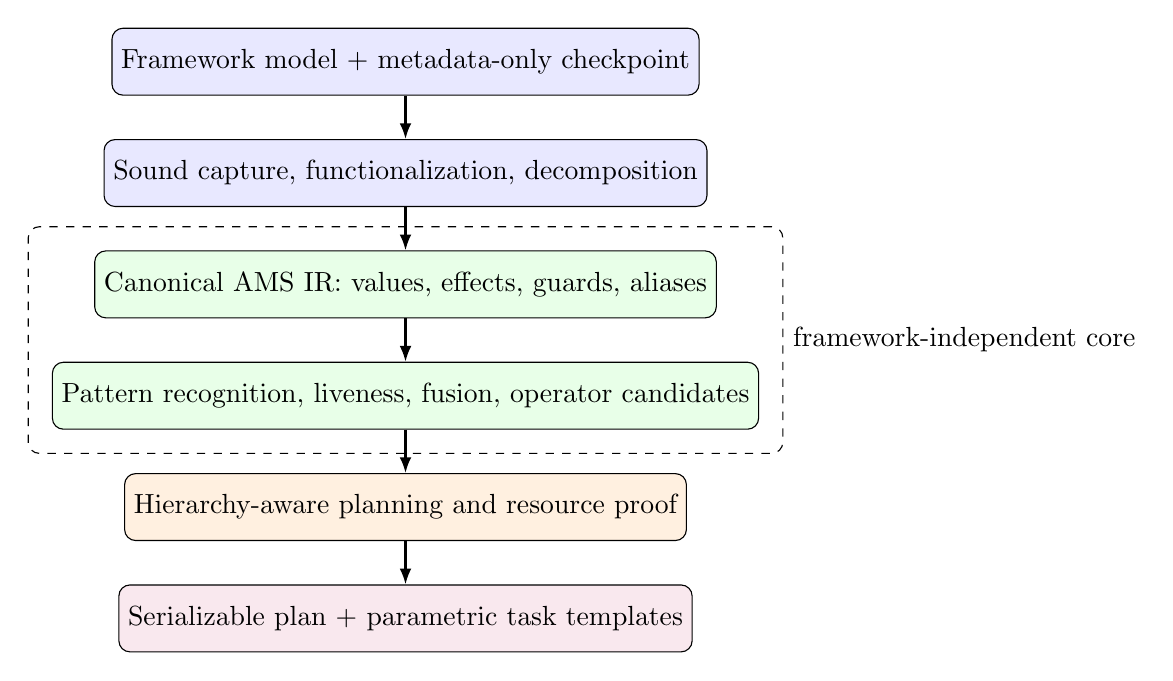
\begin{tikzpicture}[
  node distance=5.5mm,
  box/.style={draw,rounded corners,minimum width=41mm,minimum height=8.5mm,align=center},
  arr/.style={-{Latex[length=2mm]},thick}
]
  \node[box,fill=blue!9] (model) {Framework model + metadata-only checkpoint};
  \node[box,fill=blue!9,below=of model] (export) {Sound capture, functionalization, decomposition};
  \node[box,fill=green!9,below=of export] (ir) {Canonical AMS IR: values, effects, guards, aliases};
  \node[box,fill=green!9,below=of ir] (passes) {Pattern recognition, liveness, fusion, operator candidates};
  \node[box,fill=orange!12,below=of passes] (plan) {Hierarchy-aware planning and resource proof};
  \node[box,fill=purple!9,below=of plan] (exec) {Serializable plan + parametric task templates};
  \draw[arr] (model) -- (export);
  \draw[arr] (export) -- (ir);
  \draw[arr] (ir) -- (passes);
  \draw[arr] (passes) -- (plan);
  \draw[arr] (plan) -- (exec);
  \node[draw,dashed,rounded corners,fit=(ir)(passes),inner sep=3mm,label=right:{framework-independent core}] {};
\end{tikzpicture}%
}
\caption{The automated transformer operates on a functional graph and virtual storage, not only on module classes.}
\label{fig:compiler}
\end{figure}

\section{Inference Engine}
\label{sec:inference}

The inference engine applies the compiler and runtime to finite autoregressive requests. The capacity invariant applies to both prompt processing and token generation, including KV state and vocabulary operations.

\subsection{Request model}

A request descriptor contains:

\begin{itemize}
  \item token IDs or a bounded token stream;
  \item maximum prompt and generation lengths;
  \item sampling and logits-processing policy;
  \item beam, speculative, prefix-sharing, and session options;
  \item numerical and deterministic mode;
  \item latency/throughput priority and resource quota;
  \item durable-session and cancellation policy.
\end{itemize}

The request state includes current token position, RNG counters, stop automaton, KV page table, optional recurrent state, output sink, and plan phase. This state is finite under the request envelope and is stored as virtual tensors and small metadata.

\subsection{Model opening and cold start}

Opening a model validates manifests, hashes, layouts, tokenizer compatibility, graph/operator versions, and signature policy. It does not load the complete checkpoint. The engine maps metadata, opens storage handles, reserves runtime bases, loads or produces a plan, and optionally warms selected kernels and hot tiles.

A cold-start trace distinguishes:

\begin{enumerate}
  \item manifest and graph validation;
  \item conversion/repacking, if required;
  \item plan generation and calibration;
  \item kernel compilation;
  \item first physical checkpoint reads;
  \item steady-state request execution.
\end{enumerate}

Benchmark reports must not mix one-time conversion with per-request latency unless measuring deployment cold start.

\subsection{Prefill}

Prompt prefill is processed in token chunks bounded by the plan. For each transformer block, a high-performance path may stream weight panels while computing several token rows, produce Q/K/V tiles, append K/V pages, and execute tiled attention. A low-memory path spills activation tiles between projections and layers.

The activation frontier can be reduced by processing one token block through the complete layer stack, but causal attention requires access to earlier K/V state, which is virtualized. Alternative layer-major schedules may reuse weights across prompt blocks but require storing more intermediate state. The planner compares these choices.

For exact prompt logits at every token, outputs are committed for all requested positions. For ordinary generation, only positions required by the API need pass through the LM head, reducing vocabulary projection work.

\subsection{Decode}

Each decode step is a finite graph:

\begin{enumerate}
  \item embed the current token and position;
  \item execute all model blocks, reading weight tiles and prior state;
  \item append new K/V or recurrent state;
  \item stream the LM head and selection/softmax policy;
  \item draw or choose the next token;
  \item update stop state and commit the token boundary.
\end{enumerate}

The token boundary is the primary safe point. A plan switch, durable session checkpoint, resource resize, or cancellation can occur after all state for token $t$ is committed and before token $t+1$ begins.

For a model much larger than all cacheable memory, decode may reread most dense weights each token. The runtime exposes a per-token model-bytes-read metric and lower-bound-normalized bandwidth utilization so users see the physical reason for latency.

\subsection{Continuous batching and weight amortization}

Although one request establishes local executability, throughput improves when multiple requests share streamed weights. The scheduler groups decode-ready tokens with compatible model version, plan, position/mask class, and numeric mode. A weight tile is loaded once and applied to a token cohort. Cohort size is bounded by activation and KV budgets.

Continuous batching must not delay a latency-critical request indefinitely. Each request has a maximum batching wait and deadline slack. Cohorts can be split at tile boundaries; request-specific accumulators and state remain isolated.

Prefill and decode compete differently for resources. The policy may reserve a decode lane of device and IO credits while admitting prefill opportunistically. Chunked prefill prevents one long prompt from monopolizing the model sweep.

\subsection{Weight cache policy}

A cache hierarchy can retain:

\begin{itemize}
  \item small normalization and bias tensors;
  \item first/last layers important to latency;
  \item frequently reused attention or MLP panels;
  \item hot experts under observed routing;
  \item entire layers or model when capacity permits;
  \item backend-specific decoded/packed tiles.
\end{itemize}

The engine compares reuse value against KV and accumulator pressure. Cache admission is optional and revocable; no correctness path assumes a hit. Learned or profile-guided policies may be plugins, but a deterministic cost-aware policy remains the baseline.

\subsection{KV tiering and context growth}

A KV page begins in the fastest practical tier, ages to host cache, and may spill to persistent storage. Attention prefetches pages in logical order or according to sparse mask structure. Prefix pages are immutable and reference-counted; beam branches share pages until copy-on-write.

Capacity preflight uses the maximum context and concurrent-request envelope. If the user asks for an unbounded session, the API must require a retention policy: finite context window, recurrent compression, external session storage with bounded active range, or explicit per-token growth until a storage quota stops admission. The invariant does not turn an unbounded state process into a finite one.

\subsection{Speculative and beam decoding}

Speculative decoding introduces draft state and verification batches. Each branch has versioned KV deltas. Accepted tokens atomically promote their pages; rejected deltas are released after in-flight events. The target model's exact acceptance semantics are preserved. The planner accounts for worst-case speculative width and may disable speculation under minimal budgets.

Beam search shares prefix pages and maintains per-beam scores and parent pointers. Vocabulary top-$k$ can stream candidates across beams. Exact beam pruning requires a global candidate comparison, implemented by bounded heaps and external runs if the candidate set exceeds host memory.

\subsection{Output and backpressure}

Generated tokens are written to an output sink with bounded buffering. If the caller stops reading, the engine applies backpressure and eventually pauses request admission at a token boundary; it does not accumulate an unbounded output queue. Text decoding may be incremental, but tokenizer state and byte fragments are included in request memory.

\subsection{CPU-only and no-accelerator operation}

The CPU backend uses a bounded DRAM arena and memory-mapped or direct checkpoint reads. It may call BLAS for tiles or use vectorized kernels; the scalar interpreter is the final fallback. A model larger than DRAM can therefore execute directly from storage, subject to the same finite-capacity and operator conditions. GPU-specific concepts such as pinned staging collapse to simpler paths, but plan and virtual-tensor semantics are unchanged.

\subsection{Session durability}

A durable session checkpoint contains model version, committed token ordinal, token history or sufficient tokenizer state, RNG counter, KV/recurrent virtual region map, checksums, sampling policy, and plan compatibility metadata. It is committed at a token boundary. Recovery may use a different tile plan or backend because logical state is independent of physical device buffers.

\subsection{Inference acceptance contract}

For every model in the conformance suite and every finite request within a declared envelope, an accepted release must demonstrate:

\begin{itemize}
  \item completion on a configuration where the checkpoint exceeds accelerator memory;
  \item completion on at least one configuration where the checkpoint exceeds host DRAM and resides partly on storage;
  \item measured managed peak memory within the plan bound plus an explicitly defined measurement tolerance;
  \item output parity with the reference mode;
  \item cleanup to baseline after success, cancellation, and injected failure;
  \item stable error classification when preconditions do not hold.
\end{itemize}

\section{Training and Fine-Tuning Extension}
\label{sec:training}

Inference is the first implementation target, but the same virtual-tensor model extends to training. Training introduces gradients, saved activations, optimizer state, mutable parameter versions, and stricter transaction requirements. The time and storage costs can be enormous; nevertheless, finite external-memory evaluation remains possible under the same primitive assumptions.

\subsection{Linear backward sweep}

For $Y=XW^{\mathsf T}+b$ and upstream gradient $G=\partial L/\partial Y$,
\begin{align}
  \frac{\partial L}{\partial X} &= GW,\label{eq:dx}\\
  \frac{\partial L}{\partial W} &= G^{\mathsf T}X,\label{eq:dw}\\
  \frac{\partial L}{\partial b} &= \sum_{r=1}^{p}G_{r,:}.\label{eq:db}
\end{align}
Each is a tiled contraction or reduction. For a weight-gradient tile $(I_b,J_c)$,
\[
  D W_{I_b,J_c}
  =\sum_a G_{P_a,I_b}^{\mathsf T}X_{P_a,J_c}.
\]
The gradient accumulator is committed only after all microbatch/token blocks are processed. $DX$ can be produced in input-coordinate tiles by sweeping output blocks. Bias gradients use a mergeable sum.

\subsection{Autograd integration}

The canonical training IR makes backward explicit through AOT differentiation or operator-provided rules. Every operator plugin declares:

\begin{itemize}
  \item which forward values or summaries are needed by backward;
  \item whether they may be recomputed exactly and the RNG/state required;
  \item backward stream plans and resource bounds;
  \item gradient accumulation semantics and dtype;
  \item mutation/version effects.
\end{itemize}

A compatibility path may wrap an \AMS operator in a custom PyTorch autograd function, but saved tensors must be virtual handles, not hidden device tensors. The guaranteed implementation lowers the joint forward/backward graph and plans both phases together.

\subsection{Activation spill and rematerialization}

Training can trade memory for IO by spilling activations and for compute by rematerializing them. Activation checkpointing \cite{chen2016sublinear}, Checkmate \cite{jain2019checkmate}, and dynamic tensor rematerialization \cite{kirisame2020dtr} provide established trade-off frameworks. \AMS incorporates both actions into the same plan space:

\begin{itemize}
  \item \code{KEEP}: retain a tile in an admitted cache;
  \item \code{SPILL}: write a lossless virtual tile and read it in backward;
  \item \code{REMATERIALIZE}: discard and recompute from a checkpoint frontier;
  \item \code{HYBRID}: spill expensive or non-deterministic values and recompute cheap deterministic ones.
\end{itemize}

The planner accounts for parameter rereads during rematerialization. On storage-bound hardware, spilling a compact activation may be cheaper than replaying several weight sweeps. On compute-rich, bandwidth-limited hardware, the opposite may hold.

\subsection{RNG and stochastic operators}

Dropout and stochastic layers use counter-based RNG keyed by global training step, microbatch, operator instance, logical element coordinates, and recomputation epoch policy. Rematerialization reproduces the same mask without storing it. The RNG counter mapping is part of the numerical contract and checkpoint format.

Data-loader randomness, augmentation state, gradient-scaler state, and optimizer schedules are checkpointed at step boundaries. Non-deterministic custom operators cannot be rematerialized under strict mode unless they save sufficient state.

\subsection{Microbatch and gradient accumulation}

A large logical batch is partitioned into finite microbatches. Gradients are accumulated in virtual tiles across microbatches. The optimizer step is not visible until all required gradient contributions, clipping statistics, overflow checks, and distributed reductions complete.

Global norm clipping uses a streamed sum of squared gradient tiles followed by a second pass to scale/update. Mixed-precision overflow detection is a streamed logical OR over non-finite checks. Dynamic loss-scale changes are committed with the optimizer transaction.

\subsection{Optimizer-state streaming}

For Adam-like optimization, every parameter tile has associated first moment, second moment, optional FP32 master parameter, and step metadata. A tile update is:
\begin{align}
  m_t &= \beta_1m_{t-1}+(1-\beta_1)g_t,\\
  v_t &= \beta_2v_{t-1}+(1-\beta_2)g_t^2,\\
  \theta_t &= \theta_{t-1}-\eta\,
  \frac{\widehat m_t}{\sqrt{\widehat v_t}+\epsilon}.
\end{align}
The runtime streams aligned $(\theta,m,v,g)$ tiles, computes the update on CPU or accelerator, and transactionally writes new versions. Optimizer state need never reside in full in fast memory. ZeRO and ZeRO-Infinity demonstrate the value of partitioning and heterogeneous offload for training state \cite{rajbhandari2020zero,rajbhandari2021zeroinfinity}; \AMS applies its bounded tile contract even on one local node.

The optimizer plugin declares whether update order across parameter tiles is semantically observable. Ordinary independent per-element optimizers can update in any tile order after global statistics complete. Optimizers with cross-parameter coupling require a streamed global summary or explicit ordering.

\subsection{Transactional step commit}

Training mutates durable model state. The reference protocol is:

\begin{enumerate}
  \item assign step transaction ID $s$ and retain parameter version $s-1$;
  \item compute and durably stage gradient tiles or ensure they are reproducible;
  \item compute global reductions such as norm and overflow status;
  \item produce new optimizer and parameter tiles into version-$s$ regions with checksums;
  \item write a manifest delta listing all new tile versions and complete training state;
  \item atomically publish the step-$s$ root manifest;
  \item reclaim old versions according to retention policy.
\end{enumerate}

A crash before publication leaves step $s-1$ authoritative. The journal permits cleanup or completion of orphaned writes. Checkpoint consolidation into ordinary framework formats is a separate streaming export operation.

\subsection{Distributed training composition}

When multiple devices or nodes are available, parameters, gradients, optimizer state, activation tiles, and data batches may be sharded. FSDP and ZeRO reduce redundancy across workers \cite{zhao2023fsdp,rajbhandari2020zero}. \AMS treats remote shards and collectives as additional placements/tasks while preserving a local external-storage fallback. The distributed planner includes communication buffers and collective workspaces in resource vectors.

\subsection{Training-specific limitations}

A finite training step is externally evaluable, but a full open-ended training run is not finite without a step bound. Storage endurance, checkpoint write volume, and optimizer traffic may dominate. Exact reproducibility across different tile reductions may require slower deterministic modes. Consequently, the first enterprise release should make inference generally available and mark training operator coverage explicitly, rather than claim universal training before backward and transaction conformance are complete.

\section{Multi-Device and Distributed Composition}
\label{sec:multidevice}

The local invariant does not require multiple accelerators, but additional devices should enlarge tiles and reduce elapsed time without changing graph semantics. The same plan model represents intra-node and optional inter-node communication.

\subsection{Topology model}

The backend reports a directed topology graph with device memories, host NUMA nodes, peer links, PCIe switches, network interfaces, and storage affinities. Each edge has calibrated bandwidth, latency, concurrency, direct-access capability, and failure domain. A placement that causes every tile to cross a slow NUMA or PCIe path may be worse than using one device.

CPU cores and memory are also topology resources. Pinned staging should be allocated on the NUMA node nearest the target device, and storage queues should preserve affinity where the platform exposes it.

\subsection{Linear parallelization choices}

For $Y=XW^{\mathsf T}$:

\paragraph{Output partitioning.}
Partition $I_b$ across devices. Each device reads its weight rows and produces disjoint output coordinates, requiring no numeric reduction. Inputs may be replicated or streamed to each device. This is the preferred exact composition when output slices are independent.

\paragraph{Reduction partitioning.}
Partition $J_c$ across devices. Each produces a partial $Y$ tile, followed by a reduction. This can balance a very wide row but incurs communication and floating-order considerations.

\paragraph{Token partitioning.}
Partition $P_a$ across devices or requests. Each device executes independent token rows but may duplicate weight reads. It is effective when weights are locally cached or storage paths are independent.

\paragraph{Layer pipeline.}
Assign consecutive layers to devices and stream activation tiles between them. This reduces weight movement but introduces pipeline bubbles and requires each assigned layer's minimum tile plan to fit its device.

The planner may combine these dimensions and uses established tensor/pipeline parallel ideas from Megatron-class systems \cite{shoeybi2019megatron,narayanan2021efficient}.

\subsection{Distributed virtual tensors}

A physical region map may list replicas or shards on several local devices and optional nodes. Read selection considers version, locality, load, and integrity. Mutable tiles use an ownership or reduction protocol. A node failure is outside the strict single-machine invariant but can be handled by durable replicas or recomputation.

Remote transfer is an explicit task with leased network buffers and timeout/retry policy. The runtime does not expose a remote pointer as if it were local device memory. A distributed plan records topology assumptions and is invalidated when membership changes unless it has an elasticity rule.

\subsection{Collective memory discipline}

Communication libraries often allocate hidden buffers and communicators. Guaranteed mode initializes communicators during preflight, measures or configures fixed internal reserves, and uses caller-provided collective buffers where possible. Collective algorithms are locked for the plan envelope. A library that performs unbounded lazy allocation during requests is confined to best-effort mode or isolated behind a reserved pool.

\subsection{Heterogeneous devices}

Different devices may use different dtypes, kernel packs, and tile shapes. The canonical logical dtype and numeric mode determine legal conversions. Output partitioning can avoid cross-device reduction and tolerate heterogeneous throughput; the scheduler assigns tile counts proportional to calibrated rates. Reduction partitioning requires a common accumulation/merge representation.

A weak integrated GPU, discrete GPU, and CPU can all contribute, but using a slow device is optional. The planner includes transfer costs and may leave it idle. Hardware agnosticism is not mandatory load balancing.

\subsection{Graceful scaling}

A single-device plan is always retained when preconditions hold. Adding devices permits:

\begin{itemize}
  \item larger resident caches and tile dimensions;
  \item more weight/activation/KV pages concurrently resident;
  \item parallel output or token partitions;
  \item higher pipeline depth and IO concurrency;
  \item layer residency and reduced storage traffic.
\end{itemize}

Removing a device requires a safe-point replan unless the plan contains redundant tasks and dynamic ownership. The logical session state remains portable because no checkpoint or KV address is defined solely by a transient device pointer.

\section{Numerical Semantics, Stability, and Reproducibility}
\label{sec:numerics}

Tiling changes the grouping and possibly the order of floating-point operations. A correct system must state whether it preserves a scalar order, provides a bounded numerically equivalent result, or intentionally approximates the model.

\subsection{Floating-point model}

For a basic operation $\circ$, use the standard model
\[
  \fl(a\circ b)=(a\circ b)(1+\delta),\qquad |\delta|\le u,
\]
when no overflow or underflow exception invalidates the model, with unit roundoff $u$ \cite{higham2002accuracy,ieee754}. Define
\[
  \gamma_k=\frac{ku}{1-ku}
\]
for $ku<1$.

A length-$n$ sequential dot product in a fixed format has the familiar componentwise forward-error bound
\[
  |\fl(x^{\mathsf T}w)-x^{\mathsf T}w|
  \le \gamma_n |x|^{\mathsf T}|w|.
\]
This holds after accounting for the precise multiply/add or fused multiply-add model. Partitioning into tiles does not remove this error; a second-level summation of tile partials can add rounding relative to a single kernel's internal tree.

\subsection{Reduction modes}

\AMS exposes four accumulation policies.

\paragraph{Reference order.}
Reduction coordinates are processed in a canonical scalar order, and each multiply-add uses the declared primitive. This is the differential-test oracle and can target bitwise repeatability on one backend. It is slow.

\paragraph{Deterministic tree.}
The plan fixes tile partition, local kernel algorithm, and a stable pairwise merge tree. Repeated execution on the same compatible backend and software stack returns the same bits. Different backend kernels may still differ unless a cross-backend reference primitive is enforced.

\paragraph{Stable high-precision.}
Inputs may be low precision, but accumulators use FP32, FP64, or bounded integer types; reductions use pairwise or compensated summation where useful. The goal is a smaller error, not matching a conventional kernel's bits.

\paragraph{Fast equivalent.}
The backend may select efficient fused and parallel reductions within a declared tolerance. Determinism is not guaranteed if atomic or concurrent reduction order varies.

The mode is part of the plan hash. A runtime cannot switch from deterministic to fast mode under memory pressure.

\subsection{Tile-reduction error}

Suppose a dot product is divided into $r$ blocks of lengths $n_c$. Let $\widehat s_c$ be each block result and let the block results be summed sequentially. A conservative bound is
\[
  |\widehat s-s|
  \lesssim
  \sum_{c=1}^r \gamma_{n_c}|x_c|^{\mathsf T}|w_c|
  +\gamma_r\sum_{c=1}^r|\widehat s_c|.
\]
Pairwise summation of block results changes the second term to a depth-dependent bound with $O(\log r)$ stages. The planner can therefore trade accumulator workspace and synchronization for stability. Exact tests over integers or rationals verify partition logic separately from floating behavior.

\subsection{Online softmax stability}

The running-maximum recurrence in Proposition~\ref{prop:online-softmax} avoids exponentiating values above zero and is the standard stable form for streamed softmax. Accumulators $m$, $\ell$, and $O$ should generally use at least FP32 even when Q/K/V storage is FP16 or BF16. All-masked rows, infinities, NaNs, and zero normalizers require explicit semantics matching the reference framework or model contract.

Changing KV block order changes floating additions. Deterministic mode uses logical token order or a fixed merge tree. Sparse masks must not cause backend-dependent iteration order.

\subsection{Normalization stability}

LayerNorm should use Welford's recurrence or a two-pass centered variance rather than $\sum x^2-(\sum x)^2/n$ in low precision. RMSNorm sums squares in the accumulator dtype. Epsilon is applied exactly at the model-defined position. The converter preserves scalar constants without unintended dtype narrowing.

\subsection{Quantization semantics}

A quantized tensor descriptor records:

\begin{itemize}
  \item logical and storage dtype;
  \item scale and zero-point dtype and granularity;
  \item symmetric/asymmetric convention;
  \item group axes and group size;
  \item rounding and saturation rules;
  \item outlier or mixed-format representation;
  \item calibration/provenance and expected error tests.
\end{itemize}

Dequantization is a semantic operator, not a byte cast. Quantized matrix kernels must be compared to a reference implementation of the same quantized model, not automatically to the original unquantized checkpoint. Optional quantization does not alter the exact-mode executability theorem.

\subsection{Overflow, underflow, and non-finite policy}

Plans declare accumulator range assumptions. Integer quantized kernels use widths sufficient for the maximum tile reduction or periodically widen/commit partials. Floating kernels may use scaling or higher precision. Strict mode detects non-finite accumulator tiles and reports the operator, logical coordinates, input versions, and plan ID. Permissive mode propagates values according to IEEE and model semantics.

\subsection{Randomness}

Counter-based RNG is indexed by logical computation coordinates so physical task order, prefetch, and retry do not consume different random numbers. For sampling, the counter includes request ID, committed token ordinal, and sampling suboperation. For training dropout, it includes step, microbatch, operator, and element coordinates.

A retried pure task must regenerate the same random values. A task whose randomness is intentionally non-replayable is non-idempotent and requires durable output before acknowledgement.

\subsection{Numerical conformance tests}

Each operator implementation is tested in three layers:

\begin{enumerate}
  \item exact small-shape tests over integers, booleans, or high-precision arithmetic validate partitions and indexing;
  \item differential floating tests compare random and adversarial inputs against a reference implementation under mode-specific tolerances;
  \item metamorphic tests vary tile sizes, loop orders, buffer depth, storage placement, and backend while checking expected invariance or bounded deviation.
\end{enumerate}

Adversarial suites include cancellation-prone sums, extreme softmax logits, all-masked attention rows, denormals, signed zeros, NaNs/infinities, quantization boundaries, odd tails, empty tensors, and maximum declared shapes. Release reports publish both maximum observed error and tolerance rationale.

\section{Enterprise-Grade Reference Implementation}
\label{sec:enterprise}

The mathematical invariant is only useful if the implementation makes its assumptions enforceable. This section defines the architecture, operational controls, security posture, compatibility rules, and release discipline expected of a production repository. Concrete interfaces and repository layout appear in Appendices~\ref{app:interfaces} and \ref{app:repository}.

\subsection{Language and process boundaries}

A pragmatic implementation uses:

\begin{itemize}
  \item Python for public APIs, framework capture, configuration, high-level planning, and model integrations;
  \item a native core in modern C++ or Rust for arenas, leases, scheduler queues, storage IO, checksums, task state, and backend ABI;
  \item CUDA/HIP/Metal/SYCL or portable kernel code for accelerator backends;
  \item generated JSON Schema and typed models for manifests and configuration;
  \item subprocess isolation for untrusted checkpoint conversion and optional custom plugins.
\end{itemize}

The native core owns objects whose lifetime participates in the memory guarantee. Python wrappers hold opaque handles; garbage collection is not the primary release mechanism. Explicit close/cancel and context-manager semantics are mandatory, with finalizers only as leak diagnostics.

\subsection{Layered architecture}

The repository is divided into six stable layers.

\begin{enumerate}
  \item \textbf{Public API and integrations}: model opening, preflight, generation, training session, CLI, PyTorch and Transformers adapters.
  \item \textbf{Compiler}: canonical IR, importers, decompositions, shape/alias/liveness passes, operator registry, cost model, and plan serializer.
  \item \textbf{Runtime}: engine, scheduler, broker, task state machine, events, virtual tensor manager, KV manager, and transactions.
  \item \textbf{Storage}: manifest, range store, cache, AMS container, safetensors, mmap/direct IO, checksums, and optional direct-device adapters.
  \item \textbf{Backends and operators}: CPU reference, accelerator backends, kernels, codecs, and operator plugins.
  \item \textbf{Operations}: telemetry, security, fault injection, benchmark harness, packaging, CI, release, and documentation.
\end{enumerate}

Dependencies point downward. Operator plugins depend on public backend/runtime contracts, not internal scheduler classes. Framework adapters cannot reach directly into device allocators.

\subsection{Configuration}

Configuration is immutable after preflight except fields explicitly marked runtime-tunable. It includes:

\begin{itemize}
  \item tier paths, quotas, reserves, alignment, direct-IO and durability options;
  \item backend preference and forbidden devices;
  \item numerical and deterministic policy;
  \item tile/autotune limits and plan-cache policy;
  \item request concurrency, context, batching, and fairness limits;
  \item checksum, signature, encryption-at-rest integration, and plugin trust policy;
  \item telemetry destinations, redaction, and trace sampling;
  \item retry, timeout, fault, and graceful-shutdown policy.
\end{itemize}

Unknown fields are errors in strict mode. Every run records the resolved configuration with secrets removed. Environment-variable overrides map through the same schema and validation.

\subsection{Concurrency model}

The runtime uses a bounded number of long-lived worker pools:

\begin{itemize}
  \item one scheduler/control executor;
  \item storage completion and optional decompression pools with bounded queues;
  \item backend-owned transfer and compute queues/streams;
  \item telemetry export isolated from the critical path;
  \item optional conversion or verification workers.
\end{itemize}

No task creates an unbounded thread. Queue capacity is a brokered resource. Callbacks are non-blocking and enqueue state transitions; expensive work is a task. Locks have a documented order, and the lease/broker path avoids calling external code while holding global locks.

\subsection{State machines}

Request, task, lease, tile, and transaction states are explicit enums with validated transitions. For example, a task moves
\[
\begin{aligned}
\textsc{Created}&\to\textsc{WaitingDeps}\to\textsc{Ready}\\
&\to\textsc{Admitted}\to\textsc{Submitted}\\
&\to\{\textsc{Succeeded},\textsc{Failed},\textsc{Cancelled}\}.
\end{aligned}
\]
A terminal task releases leases only after all associated events are terminal. Illegal transitions produce invariant violations and crash the affected engine instance in fail-fast development mode; production isolates the request, emits a core diagnostic, and prevents reuse of suspect buffers.

State machines are model-checked or property-tested for cancellation races, duplicate completions, event reordering, and shutdown. The scheduler's reference model is small enough for exhaustive exploration at low task counts.

\subsection{Reliability and crash consistency}

The runtime distinguishes ephemeral inference, durable inference sessions, and training. Ephemeral inference needs cleanup and integrity but may not fsync state. Durable sessions and training use journals and atomic manifest publication as described earlier.

Storage writes are content-addressed or versioned, never in-place over the sole valid copy. Checksums are verified at read boundaries and may be cached with authenticated file identity. A scrubber can verify idle checkpoint chunks. Storage-full conditions are preflighted and monitored; a reserved emergency segment permits journal completion and clean failure.

Graceful shutdown stops admission, cancels or completes requests according to policy, quiesces backends, commits required state, releases leases, closes stores, and flushes telemetry. Forced shutdown relies on journal recovery.

\subsection{Security model}

Model files, custom plugins, prompts, and user configuration are untrusted inputs unless explicitly trusted. Required controls include:

\begin{itemize}
  \item no default execution of checkpoint pickle or arbitrary model repository code;
  \item strict bounds and integer-overflow checks on every shape, stride, offset, length, codec expansion, and allocation formula;
  \item canonical path handling that rejects traversal and symlink policy violations;
  \item manifest and chunk checksums, optional signed root manifests, and provenance recording;
  \item decompression ratios and CPU-time quotas to prevent archive bombs;
  \item plugin allowlists, signatures, ABI validation, and optional process sandboxing;
  \item tenant quotas for memory, IO, compute, storage, context, and output;
  \item secret and prompt redaction in logs/traces; tensor bytes absent by default;
  \item fuzzing of parsers, manifests, codecs, operator attributes, and RPC/CLI inputs;
  \item software bill of materials, dependency scanning, reproducible packages where practical, and signed release artifacts.
\end{itemize}

Custom native kernels remain a high-trust extension because they execute in the process and device context. A plugin that cannot satisfy the workspace and lifetime ABI is outside the bounded-allocation guarantee.

\subsection{Compatibility and versioning}

The project follows semantic versioning for public Python APIs and separate versioning for:

\begin{itemize}
  \item canonical IR schema;
  \item plan schema;
  \item AMS container format;
  \item native plugin ABI;
  \item backend pack/cache format;
  \item telemetry event schema.
\end{itemize}

Readers support a declared backward-compatible range and reject unknown major versions. Migrations are streaming and idempotent. Plans are disposable caches and may be regenerated; canonical checkpoints and session state require durable migration tooling.

A compatibility matrix lists Python, PyTorch, compiler, OS, driver, backend, architecture, and filesystem versions. Unsupported combinations fail preflight with the matrix rule, not with an arbitrary kernel error.

\subsection{API stability and extension points}

Stable public interfaces include:

\begin{itemize}
  \item \code{open\_model}, \code{preflight}, \code{generate}, \code{stream\_generate}, and session lifecycle;
  \item backend, storage, codec, operator, planner-policy, logits-processor, and telemetry plugin protocols;
  \item manifest and plan inspection CLIs;
  \item structured error codes and diagnostic payloads.
\end{itemize}

Internal tile/task classes are not public until their invariants are mature. Extension interfaces are capability-negotiated and versioned. A plugin conformance runner validates resource bounds, cancellation, numerical behavior, serialization, and thread safety before it is accepted into guaranteed mode.

\subsection{Operational tooling}

The CLI should provide:

\begin{description}[leftmargin=3.5cm,style=nextline]
  \item[\code{ams convert}] Streaming checkpoint import, repack, quantize if explicitly selected, checksum, sign, and verify.
  \item[\code{ams inspect}] Display tensor layouts, aliases, chunk ranges, graph coverage, and integrity without loading data.
  \item[\code{ams preflight}] Produce plan, exact memory/spill bounds, unsupported ops, estimated traffic, and fallback chain.
  \item[\code{ams run}] Execute generation with bounded configuration and machine-readable results.
  \item[\code{ams benchmark}] Run calibrated micro/macro suites and export a reproducibility bundle.
  \item[\code{ams trace}] Summarize critical path, bandwidth, stalls, cache, memory, and plan deviations.
  \item[\code{ams recover}] Inspect and recover journals, orphaned versions, and durable sessions.
  \item[\code{ams doctor}] Validate drivers, storage behavior, direct IO, pinned memory, clocks, permissions, and backend conformance.
\end{description}

All commands have JSON output and stable exit codes for automation.

\subsection{Documentation standard}

Documentation includes architecture decision records, contributor setup, API references, operator authoring guide, backend guide, checkpoint format, security model, performance tuning, numerical semantics, failure catalog, runbooks, and model-support matrix. Every claimed guarantee links to its preconditions and corresponding tests. Examples use small redistributable checkpoints or synthetic tensors and run in CPU-only CI.

\subsection{Definition of enterprise readiness}

A release is enterprise-ready only when:

\begin{itemize}
  \item the core inference invariant passes the conformance hardware matrix;
  \item memory and workspace bounds are measured and reconciled with plan accounting;
  \item parsers and native core pass fuzzing and sanitizers;
  \item fault, cancellation, recovery, and storage-full tests pass;
  \item observability and error codes support incident diagnosis without debug builds;
  \item compatibility, security, backup/recovery, and upgrade documentation are complete;
  \item performance regressions are gated against stable baselines;
  \item release artifacts are signed and traceable to source and CI evidence.
\end{itemize}

\section{Verification and Evaluation Protocol}
\label{sec:verification}

The purpose of evaluation is not merely to report tokens per second. It must test the governing invariant, semantic correctness, memory accounting, progress, resilience, portability, and the predicted time--memory trade. This section is a protocol for the implementation; no unmeasured result is asserted.

\subsection{Questions}

The artifact should answer:

\begin{enumerate}
  \item Does an accepted plan complete when the model or an individual tensor exceeds accelerator memory?
  \item Does it complete when the checkpoint exceeds host DRAM and is streamed from persistent storage?
  \item Is managed peak use bounded by the preflight plan across success, cancellation, and faults?
  \item Do outputs satisfy exact/deterministic/tolerance contracts across tile sizes and placements?
  \item Does asynchronous pipelining approach the expected bottleneck stage when overlap is supported?
  \item How do latency and throughput scale as fast-memory budget decreases?
  \item Which operator, IO path, cache, or scheduler effect limits performance?
  \item Does the compiler cover real model graphs without hidden whole-tensor materialization?
  \item Are failures classified, cleaned up, and recoverable?
\end{enumerate}

\subsection{Unit and property tests}

Each pure component has deterministic unit tests. Property-based generators cover shapes, dtypes, strides, partitions, budgets, and fault sequences. Required properties include:

\begin{itemize}
  \item virtual tile round-trip preserves logical values and aliases;
  \item partition plans cover domains exactly once and tails correctly;
  \item every accepted task vector fits and every lease is eventually released;
  \item buffer epochs prevent reuse before completion;
  \item online summaries equal batch references in exact arithmetic;
  \item plan serialization is canonical and round-trips;
  \item manifest parsers reject overflow, overlap, truncation, duplicate IDs, and invalid codecs;
  \item cancellation at every state reaches a terminal request with baseline resources;
  \item transaction recovery selects the last fully published version.
\end{itemize}

A reference scheduler model executes tasks synchronously and is compared to the concurrent scheduler's terminal state for generated DAGs. Small-state model checking explores resource vectors, event orders, retries, and cancellation.

\subsection{Operator differential tests}

For every operator/backend/mode tuple:

\begin{enumerate}
  \item generate random and adversarial logical inputs;
  \item execute a trusted whole-tensor or high-precision reference where it fits;
  \item execute many \AMS tile grids, loop orders, storage placements, and buffer depths;
  \item compare values, aliases, side effects, RNG, and errors under the declared contract;
  \item record worst observed error and resource high-water marks.
\end{enumerate}

Linear tests include prime and odd dimensions, one-scalar tiles, non-contiguous views, tied storage, zero dimensions, large reduction counts, quantized tails, and spillable output. Attention tests include causal/prefix/window masks, all-masked rows, grouped-query heads, long KV paging, shared prefixes, and storage-resident pages. MoE tests vary route imbalance and duplicate expert choices. SSM tests compare recurrent and scan plans.

Gradient tests use finite differences where practical and framework double-precision gradient references for double precision. They verify accumulation across microbatches, rematerialization RNG, optimizer updates, and crash recovery.

\subsection{Memory invariant tests}

The test harness runs the engine with deliberately small broker arenas independent of physical device capacity. For each plan it records:

\[
  \Delta_k=\peak(M_k^{\mathrm{measured}})-B_k^{\mathrm{plan}}.
\]
The managed allocator requires $\Delta_k\le0$. Device-wide telemetry may include fixed driver or external noise; its acceptance uses a separately calibrated reserve and tolerance. Any unexplained growth is a failure, not automatically added to the margin.

Tests include:

\begin{itemize}
  \item a weight matrix whose single conventional allocation exceeds the arena;
  \item input and output tensors independently larger than the arena;
  \item KV cache larger than device and host cache tiers;
  \item simultaneous requests at maximum admitted concurrency;
  \item repeated plan create/destroy cycles and long-running decode;
  \item cancellation during read, copy, kernel, reduction, and commit;
  \item external cooperative pressure causing cache shrink and safe replan;
  \item plugins attempting to exceed workspace, which must be rejected or isolated.
\end{itemize}

\subsection{Fault-injection matrix}

The storage and backend test doubles inject:

\begin{itemize}
  \item short reads, delayed completions, reordered completions, and queue saturation;
  \item checksum mismatch, stale replica, truncated file, and manifest corruption;
  \item disk full, permission change, read-only transition, and device removal;
  \item transfer failure, kernel error, event error, and communicator failure;
  \item process crash at every journal publication step;
  \item duplicate callback and lost callback simulation in debug schedulers;
  \item telemetry exporter failure and slow output consumer.
\end{itemize}

Expected outcomes specify retry limits, replica use, terminal code, durable version, and resource cleanup. Fault tests run under thread, address, undefined-behavior, and leak sanitizers where applicable.

\subsection{Hardware and software matrix}

A credible portability evaluation includes at least:

\begin{itemize}
  \item CPU-only machine with model larger than configured DRAM cache;
  \item low-memory discrete GPU, such as 8--12~GiB class;
  \item 16--24~GiB consumer GPU;
  \item high-memory data-center GPU as an all-resident upper baseline;
  \item two local GPUs with asymmetric or peer topology;
  \item one unified-memory platform where supported;
  \item CUDA and at least one non-CUDA accelerator backend once claimed stable;
  \item SATA SSD and NVMe storage, with filesystem and direct-IO variants.
\end{itemize}

The report lists CPU, memory channels, NUMA, GPU, PCIe generation/width, storage model/firmware/filesystem, OS/kernel, drivers, clocks/power policy, thermal state, framework/compiler commits, and background-load controls.

\subsection{Models and workloads}

Use both synthetic and real models.

\paragraph{Synthetic contractions.}
Dense matrices and tensor contractions at $0.5\times$, $1\times$, $2\times$, $8\times$, and $32\times$ the fast-memory budget isolate tile correctness and bandwidth. Shapes include one row larger than the arena and output larger than the arena.

\paragraph{Dense decoder models.}
Use several public transformer sizes such that at least one fits device memory, one exceeds device memory but fits DRAM, and one exceeds configured DRAM cache and streams from storage. Include multi-query/grouped-query attention and large-vocabulary cases.

\paragraph{MoE model.}
Evaluate balanced and adversarial routing, hot-expert caching, and worst-case all-expert traffic.

\paragraph{State-space or recurrent model.}
Compare recurrent decode and chunked prefill plans.

\paragraph{Training microbenchmarks.}
After training support is stable, test LoRA/adapters and full linear backward, then a small end-to-end model with optimizer streaming and recovery.

Workloads cover prefill lengths, decode lengths, batch/concurrency, cold and warm cache, deterministic and fast modes, and optional quantization.

\subsection{Baselines}

Relevant baselines are selected according to the question:

\begin{itemize}
  \item ordinary framework execution when the model fits;
  \item naive whole-layer CPU/disk offload;
  \item Hugging Face Accelerate big-model inference \cite{accelerate_big_model};
  \item DeepSpeed ZeRO-Inference \cite{deepspeed_zero_inference};
  \item FlexGen for throughput-oriented heterogeneous inference \cite{sheng2023flexgen};
  \item llama.cpp CPU/GPU offload and quantized local inference \cite{llamacpp};
  \item vLLM for all-resident or supported KV-paged serving \cite{kwon2023pagedattention};
  \item ZeRO/FSDP/ZeRO-Infinity for training questions \cite{rajbhandari2020zero,zhao2023fsdp,rajbhandari2021zeroinfinity}.
\end{itemize}

Baselines must use comparable precision, quantization, batch, context, output length, and correctness. If a baseline cannot run because one layer exceeds its unit of offload, report that fact separately from throughput.

\subsection{Metrics}

Primary metrics are:

\begin{itemize}
  \item completion and error classification;
  \item managed and process/device peak bytes by tier;
  \item checkpoint, link, spill, and KV bytes per prompt/token;
  \item time to first token, inter-token latency distribution, and total latency;
  \item prompt and generation throughput;
  \item storage/link bandwidth utilization and read-size distribution;
  \item compute utilization, kernel launch count, and achieved operation rate;
  \item overlap efficiency and idle/stall decomposition;
  \item cache hit and prefetch precision;
  \item numerical error or exact-match rate;
  \item energy and storage write volume where measurable;
  \item recovery time and leaked-resource count after faults.
\end{itemize}

Plot performance against the configured fast-memory budget to reveal the trade curve. Report cold and warm conditions separately. Include confidence intervals over repeated runs and explain cache flushing and thermal controls.

\subsection{Acceptance thresholds}

Initial release gates should be objective but not fabricate throughput targets:

\begin{enumerate}
  \item \textbf{Correctness}: all exact/property tests pass; floating errors stay within mode-specific published tolerances.
  \item \textbf{Capacity}: every accepted invariant test completes with managed peak at or below plan bounds.
  \item \textbf{Fallback}: candidate generation reaches a valid minimum plan for every supported operator under its documented minimum budget.
  \item \textbf{Cleanup}: no lease, file descriptor, thread, stream, or page remains owned after terminal cleanup.
  \item \textbf{Recovery}: fault cases recover the last committed version and emit the specified code.
  \item \textbf{Performance sanity}: overlappable pipelines show no unexplained serialization; calibrated estimates remain within a published error band on stable microbenchmarks.
  \item \textbf{Regression}: protected benchmark medians and tails do not regress beyond repository thresholds without an approved baseline update.
\end{enumerate}

\subsection{Reproducibility bundle}

Each benchmark run exports configuration, plan, graph/checkpoint hashes, hardware/software inventory, calibration database, raw metrics, task trace, logs, command line, random seeds, and analysis scripts. Checkpoint licenses may prevent redistribution, but content hashes and acquisition instructions remain. The paper's final empirical version should archive this bundle in a durable repository.

\section{Related Work}
\label{sec:related}

\subsection{External-memory and IO-aware computation}

The red--blue pebble game formalizes communication between memory levels and establishes lower bounds for numerical algorithms \cite{hong1981io}. \AMS follows this tradition by making physical traffic and bounded local storage part of the computation model. Its external-memory theorem is elementary; the systems contribution is to turn that principle into an LLM-wide operator, compiler, and runtime contract.

FlashAttention tiles exact attention to reduce transfers between HBM and on-chip SRAM and analyzes IO complexity \cite{dao2022flashattention,dao2023flashattention2}. \AMS uses the same online-softmax algebra but introduces slower tiers and virtualizes Q/K/V, KV state, parameters, and outputs. Welder's tile-graph compiler coordinates fine-grained data reuse and can combine accelerator and host memory for large inputs \cite{shi2023welder}. \AMS is complementary: it makes bounded-residency executability a hard per-operator contract and includes persistent storage, runtime admission, failure semantics, and a scalar fallback.

\subsection{LLM inference offload}

FlexGen jointly places weights, activations, and attention cache across GPU, CPU, and disk and uses a cost optimization for throughput-oriented inference \cite{sheng2023flexgen}. It is the closest systems antecedent to \AMS. \AMS differs in emphasis and scope: it requires sub-tensor decomposition even when an individual layer/tensor does not fit, defines a general operator plugin contract and memory proof, virtualizes outputs and all state classes, and specifies a portable production runtime rather than one model-family execution engine.

LLM in a Flash stores weights in flash and optimizes transferred bytes and contiguous read size using sparsity-aware techniques \cite{alizadeh2023llmflash}. PowerInfer exploits hot/cold neuron locality across GPU and CPU \cite{song2023powerinfer}. ZeRO-Inference offloads model weights and KV state and supports quantization \cite{deepspeed_zero_inference}. Hugging Face Accelerate dispatches layers across accelerators, CPU, and disk \cite{accelerate_big_model}. llama.cpp provides widely used quantized CPU/GPU local inference and layer offload \cite{llamacpp}. \AMS does not replace their optimized paths; its invariant requires a deeper fallback when the chosen unit of placement itself does not fit.

Petals distributes model blocks across participating machines \cite{borzunov2022petals}. It addresses access through collaborative resources rather than a strictly local hierarchy, but its remote blocks can be viewed as an optional placement tier.

\subsection{KV memory virtualization}

vLLM's PagedAttention applies virtual-memory concepts to KV-cache allocation and sharing \cite{kwon2023pagedattention}. vTensor uses GPU virtual memory management to decouple logical tensor allocation from physical GPU pages. These systems focus primarily on serving-time dynamic KV or tensor memory inside GPU/host domains. \AMS adopts page-table ideas but applies one virtual tensor/version/resource contract to parameters, activations, outputs, KV, gradients, optimizer state, and persistent storage.

\subsection{Training memory systems}

ZeRO partitions optimizer, gradient, and parameter state across data-parallel workers \cite{rajbhandari2020zero}; ZeRO-Infinity adds CPU and NVMe offload \cite{rajbhandari2021zeroinfinity}. PyTorch FSDP provides industry-grade sharded training integrated with framework internals \cite{zhao2023fsdp}. vDNN, SuperNeurons, and SwapAdvisor virtualize or schedule activation memory and swapping for training \cite{rhu2016vdnn,wang2018superneurons,huang2020swapadvisor}. Activation checkpointing, Checkmate, and dynamic tensor rematerialization trade recomputation for saved activation memory \cite{chen2016sublinear,jain2019checkmate,kirisame2020dtr}. \AMS combines spill and recomputation in a common virtual-tensor plan and extends the minimum-tile invariant to operator parameters and outputs.

\subsection{Parallelism}

Megatron-LM and related systems use tensor and pipeline parallelism to distribute large language models across accelerators \cite{shoeybi2019megatron,narayanan2021efficient}. These approaches increase aggregate fast memory and throughput. \AMS composes with them but retains a one-machine external-memory fallback; adding hardware enlarges tiles and caches rather than changing logical semantics.

\subsection{Architectures}

Transformers define the principal attention/MLP workload \cite{vaswani2017attention}. Sparse MoE architectures such as Switch Transformers and Mixtral change the set of active expert parameters \cite{fedus2021switch,jiang2024mixtral}. Mamba and related state-space models use recurrent/scan structure \cite{gu2023mamba}. \AMS does not assume one architecture: each semantic operator supplies a bounded stream plan and primitive fallback.

\subsection{Positioning of novelty}

The ingredients of \AMS have extensive precedent. The defensible novelty is their composition around a testable invariant:

\begin{quote}
Every supported material tensor is virtual, every supported operator has a minimum-working-set plan, every task is resource-admitted, and every accepted finite request has a bounded-residency path whose fast-memory requirement is independent of total parameter size.
\end{quote}

Whether this composition yields publishable empirical value depends on implementation quality and evaluation. The paper deliberately avoids claiming that tiling or offload itself is new.

\section{Limitations and No-Free-Lunch Boundaries}
\label{sec:limitations}

\subsection{Storage capacity remains finite}

``Any LLM'' means any finite supported model whose representation and spill fit the configured hierarchy. A fixed disk cannot hold an arbitrarily large checkpoint. An unbounded conversation or training run needs a retention or quota policy. The runtime can move the capacity boundary to a slower/larger tier; it cannot remove finite storage.

\subsection{Minimum working set is nonzero}

Every primitive needs operands, result space, metadata, and executable state. A GPU may be too constrained or unsupported even for the smallest legal kernel. The CPU scalar fallback reduces the requirement but still needs process and OS memory. If no backend can reserve its minimum, preflight correctly rejects the request.

\subsection{Time can be prohibitive}

The dense read lower bound means a model streamed from storage may require reading most parameter information for each non-amortized pass. At batch-one decode, this can make token latency proportional to model bytes divided by effective bandwidth. Tiny tiles also incur seek, launch, synchronization, and underutilization costs. \AMS guarantees a path, not interactivity.

\subsection{Persistent-storage endurance and energy}

Inference is primarily read-heavy, but KV spill, activation spill, durable sessions, and training generate writes. High write amplification can consume SSD endurance and energy. The planner should report projected writes and support read-only or write-budget policies. No storage device is assumed to have infinite endurance.

\subsection{Operator coverage is a real boundary}

Opaque custom kernels, arbitrary Python side effects, data-dependent native allocations, and external services may not be stream-decomposable through the registered primitive set. The compiler must reject uncovered paths. Claiming universal support by falling back to ordinary execution would reintroduce the same residency failure.

\subsection{Shared-system interference}

A user-space reservation can control its arenas but not arbitrary peer processes, drivers, display servers, kernel memory, thermal throttling, or device resets. Exclusive deployment improves the operational guarantee. Cooperative pressure can trigger a safe replan; non-cooperative revocation is a terminal environmental failure.

\subsection{Floating-point identity}

Different tile shapes and parallel reductions can alter floating-point rounding. Exact real-arithmetic correctness does not imply bitwise identity with a monolithic vendor kernel. The system exposes deterministic and tolerance modes, but cross-platform identical bits may require slow reference primitives.

\subsection{Data confidentiality}

Checkpoint and activation spill expands the set of storage locations containing sensitive data. Encryption, secure deletion, access control, tenant isolation, and crash-dump policy are deployment responsibilities supported by adapters but not solved by tiling alone. Direct IO and memory mapping have platform-specific security considerations.

\subsection{Planning complexity and calibration drift}

The plan space is large, and cost models can be wrong under contention, firmware changes, thermal limits, or filesystem cache effects. Safe fit does not depend on cost accuracy, but performance does. Plans and calibrations must be versioned, traced, and invalidated conservatively.

\subsection{Graph capture limitations}

Framework export may fail on dynamic Python, unsupported tensor subclasses, custom dispatch, or model repository code. A native model adapter can bypass capture, but then assumes responsibility for a complete semantic graph. The project needs a transparent support matrix rather than a blanket claim about every repository called an LLM.

\subsection{Training practicality}

External-memory training is theoretically possible but may multiply model, gradient, optimizer, activation, and checkpoint IO. Full training of extremely large dense models on one local machine can be economically or temporally unreasonable. Parameter-efficient fine-tuning and distributed composition are more practical first targets.

\subsection{Novelty risk}

Prior systems already combine offload, heterogeneous memory, paging, tile scheduling, and rematerialization. A research contribution must be judged on the rigor and usefulness of the invariant, operator generality, implementation, and empirical results. Renaming existing row-wise offload would not suffice. The architecture in this paper intentionally raises the implementation bar to a complete virtual-tensor runtime.

\section{Conclusion}
\label{sec:conclusion}

Accumulative Matrix Sweeping reframes model capacity as a scheduling problem over a memory hierarchy. Its core rule is simple: logical tensors are never equated with full fast-memory allocations; every supported operator has a bounded tile program; reductions carry only bounded summaries; and all material state, including weights, activations, outputs, KV cache, gradients, optimizer state, transfer buffers, and workspaces, participates in one resource contract.

Under explicit finite-model, backing-capacity, primitive-support, and progress assumptions, a finite LLM request has an external-memory execution whose fast-memory requirement is independent of total parameter size. A preallocated arena and atomic resource admission turn this existence result into a runtime allocation bound. Two-dimensional matrix sweeping, online attention, streamed normalization and vocabulary selection, paged state, and scalar fallback make the invariant concrete across model families.

The trade is equally explicit. Exact dense computation must consume the information in its weights, and a local machine with insufficient residency can become dominated by storage and interconnect bandwidth. \AMS does not erase that cost. It replaces an abrupt out-of-memory boundary with a continuous, observable time--memory curve, while allowing stronger hardware to choose larger tiles or conventional all-resident kernels.

The appendices define the algorithms, interfaces, formats, repository, tests, and release gates needed to implement the system. The next scientific step is an open artifact and reproducible evaluation against layer offload, heterogeneous inference, KV paging, and local quantized runtimes across budgets that force sub-layer and sub-tensor execution. Only those measurements can establish where the universal fallback is practically useful and where the lower-bound costs dominate.

\appendix
\section{Detailed Proofs}
\label{app:proofs}

This appendix expands the proof sketches in Section~\ref{sec:theory}. The results are intentionally stated for finite supported computations; they do not assert a performance bound beyond finiteness.

\subsection{Scalarization of tensor programs}

\begin{lemma}[Finite scalarization]
\label{lem:scalarization}
Let $G$ be a finite executed trace of tensor operators. Suppose each operator has finite input/output shapes on the trace and a semantic definition that expands into finitely many scalar primitives from $\mathcal P$. Then $G$ expands into a finite scalar directed acyclic graph after representing loop-carried state by value versions.
\end{lemma}

\begin{proof}
Every tensor has finitely many logical elements because all dimensions are finite. By hypothesis, each operator invocation expands into finitely many scalar primitive invocations and dependencies. The executed trace has finitely many operator invocations. Their disjoint union plus edges induced by tensor element dependencies is finite. Mutation or loop-carried state is transformed into static single assignment versions for the finite trace, so dependencies point from earlier versions to later versions. A terminating sequential trace cannot contain a value-dependency cycle without a delayed state edge; versioning breaks such edges. Hence the expanded graph is finite and acyclic.
\end{proof}

\begin{lemma}[Bounded scalar evaluator]
\label{lem:scalar-evaluator}
Let $D$ be a finite scalar DAG over primitives of maximum encoded operand/result working set $\mu_{\mathcal P}$. If all inputs and a map from node identifiers to spill locations fit in backing storage, then $D$ can be evaluated with fast-memory use at most $R+\mu_{\mathcal P}+O(1)$ metadata.
\end{lemma}

\begin{proof}
Choose a topological ordering $v_1,\ldots,v_N$. Persist source values. For $i=1,
\ldots,N$, read the operands named by predecessors of $v_i$, execute the primitive, and write the result to the spill location associated with $v_i$. The evaluator stores only one primitive working set and a bounded descriptor at a time. The node-to-location map may itself reside in backing storage and be read in bounded records; alternatively, locations can be computed from a fixed-width index. Values whose final consumer has executed may be reclaimed, but reclamation is not required for the fast-memory bound. The result follows.
\end{proof}

\begin{proof}[Full proof of Theorem~\ref{thm:external-eval}]
Apply Lemma~\ref{lem:scalarization} to obtain a finite scalar DAG and Lemma~\ref{lem:scalar-evaluator} to evaluate it. Every read, primitive, and write completes in finite time by assumption, and a finite sum of finite durations is finite. The working set depends on the primitive set and runtime, not the number of parameters or DAG nodes.
\end{proof}

\begin{remark}[Metadata size]
A naive topological schedule stored entirely in fast memory would violate the stated independence for a very large graph. The construction stores graph, indices, and value-location metadata in backing storage or generates them from compact parametric loops. The runtime implementation likewise instantiates only a bounded task window.
\end{remark}

\subsection{Bounded arena proof with asynchronous work}

Let each lease $\ell$ have byte charge $r_k(\ell)$ in tier $k$ and terminal event $e(\ell)$. A lease remains active until $e(\ell)$ is terminal, even if its owning language-level object is unreachable.

\begin{lemma}[No early reuse]
\label{lem:no-early-reuse}
If an arena block is returned to the free set only after the terminal event of its current epoch, no two nonterminal operations receive overlapping writable blocks with the same epoch.
\end{lemma}

\begin{proof}
A block is absent from the free set while its lease is active. Allocation draws only from the free set and increments the block epoch. Therefore a second lease cannot receive the block before the first terminal event, and after reuse it has a distinct epoch. Debug-time epoch validation detects stale views.
\end{proof}

\begin{proof}[Full proof of Theorem~\ref{thm:memory-bound}]
At arena creation, total managed addressable bytes plus fixed reserve equal at most $C_k$. Atomic admission subtracts the class-rounded charge of every new lease from available credits and refuses when insufficient. Completion adds exactly the charge back after Lemma~\ref{lem:no-early-reuse}. By induction over admission and completion transitions, active charges never exceed arena capacity. Fixed metadata and alignment losses are included in class rounding or reserve. No task can allocate outside leases by hypothesis, and kernel workspace is a lease, so managed peak is bounded. Parameter-size independence follows because the plan fixes maximum in-flight tile sizes and represents all other regions virtually.
\end{proof}

\subsection{Scheduler progress with errors and cancellation}

Let a terminal state be success, failure, or cancellation. A failed task marks all not-yet-submitted descendants terminally cancelled unless a retry or alternative replica edge is selected. A submitted task is allowed to finish and then releases resources.

\begin{lemma}[Ready-node existence]
\label{lem:ready-node}
In a finite DAG with unfinished nodes, after treating terminal predecessors as resolved according to the error propagation rule, either a terminal request condition has been reached or at least one unfinished node is ready.
\end{lemma}

\begin{proof}
Consider the subgraph induced by unfinished nodes. If it is empty, the request is terminal. Otherwise, every finite DAG has a source. Its predecessors lie outside the unfinished subgraph and are therefore terminal/resolved, so it is ready unless the request's error rule has already made it terminal, in which case remove it and repeat.
\end{proof}

\begin{proof}[Full proof of Theorem~\ref{thm:progress}]
Let $n$ be the number of unfinished nodes. For $n=0$, the result is immediate. For $n>0$, Lemma~\ref{lem:ready-node} gives a ready node unless the request is already terminal. By the fit hypothesis and fair scheduling, some fit ready node is eventually admitted. Atomic complete-vector admission eliminates resource hold-and-wait. Eventual service makes the task terminal, and completion processing releases all leases. Error propagation may make additional nodes terminal. Thus the number of unfinished nodes decreases. Induction reaches zero. Cancellation uses the same argument after preventing new admissions and treating pending nodes as cancelled; submitted nodes complete or fail under eventual service.
\end{proof}

The fit hypothesis is enforced by compilation: every operator template has at least one minimum candidate, and the executor does not create a phase in which all ready nodes require mutually unavailable plan-specific resources. Resource classes needed only by future phases are not permanently pinned by the current phase unless included in the global feasibility simulation.

\subsection{Linear sweep correctness with spill}

For each coordinate $(r,i)$,
\[
  A_{r,i}^{(0)}=b_i,
  \qquad
  A_{r,i}^{(c+1)}=A_{r,i}^{(c)}+
  \sum_{j\in J_c}X_{r,j}W_{i,j}.
\]
By induction,
\[
  A_{r,i}^{(q)}=b_i+
  \sum_{c=0}^{q-1}\sum_{j\in J_c}X_{r,j}W_{i,j}.
\]
Because the $J_c$ form a disjoint cover, this is $b_i+\sum_{j=0}^{n-1}X_{r,j}W_{i,j}$. Writing $A^{(c)}$ to external storage and reading it before the next update is an identity transformation in the exact storage model. Checksums and version IDs ensure the implementation reads the same value.

If reduction blocks are processed in parallel, each worker $s$ returns
\[
  A^{[s]}_{r,i}=\sum_{j\in J^{[s]}}X_{r,j}W_{i,j}.
\]
A final reduction over a disjoint cover plus one bias application is algebraically identical. Floating order is governed separately.

\subsection{Online softmax proof for blocks}

Let $A$ be the set of scores processed before a block and $B$ the new scores. Assume
\[
  m_A=\max_{j\in A}s_j,
  \quad \ell_A=\sum_{j\in A}e^{s_j-m_A},
  \quad O_A=\sum_{j\in A}e^{s_j-m_A}V_j.
\]
Set $m=\max(m_A,\max_{j\in B}s_j)$. Then
\[
  e^{m_A-m}\ell_A
  =\sum_{j\in A}e^{s_j-m}
\]
and similarly for $O_A$. Adding the $B$ terms yields the invariant for $A\cup B$. At completion,
\[
  \frac{O}{\ell}
  =\frac{\sum_j e^{s_j-m}V_j}{\sum_j e^{s_j-m}}
  =\sum_j\operatorname{softmax}(s)_jV_j.
\]
Masked entries are omitted or assigned score $-\infty$. If all entries are masked, the model/framework-specific result must be defined separately because the mathematical denominator is zero.

\subsection{Dense read lower bound and representations}

Theorem~\ref{thm:dense-lower-bound} is stated in terms of inspecting entries or information sufficient to distinguish them. This accommodates compressed representations. Lossless compression may encode several entries jointly; the algorithm need not read $mn$ physical words, but it must consume enough information to distinguish every arbitrary matrix in the supported set. For a fixed finite field with $q$ values, arbitrary matrices contain $mn\log_2q$ bits of information. A representation-specific lower bound follows from its code length. Structured, sparse, generated, or lossy models restrict the set and can evade the arbitrary-dense premise.

\subsection{Fast-memory independence versus total storage}

The theorems do not say that total memory use is independent of model size. Backing storage contains at least the model representation, and a naive scalar evaluator may spill many intermediates. The precise claim is that the capacity of the compute-nearest admitted working set need not scale with the total parameter bytes. Practical plans also bound host cache and pinned memory independently, while slow-tier capacity scales with model and request state.

\section{Reference Algorithms}
\label{app:algorithms}

These algorithms define semantics and control flow. An implementation may optimize them while preserving dependencies, resources, and numerical contracts.

\subsection{Preflight}

Algorithm~\ref{alg:preflight} validates the package, request envelope, backing capacity, backend reserve, operator coverage, and resource proof before any model execution begins.

\begin{algorithm}[H]
\caption{Model and request preflight}
\label{alg:preflight}
\begin{algorithmic}[1]
\Require Model package $M$, request envelope $R$, hierarchy $H$, policy $\Pi$
\State $V\gets\Call{ValidateManifestAndGraph}{M,\Pi.security}$
\If{$V$ fails} \State \Return structured rejection \EndIf
\State $S\gets\Call{BoundSlowTierState}{M,R,\Pi}$
\If{no storage placement can hold $S$} \State \Return \code{PREFLIGHT\_NO\_BACKING} \EndIf
\State $C\gets\Call{DiscoverAndCalibrateCapabilities}{H,\Pi}$
\ForAll{backend sets $B$ in preferred fallback order}
  \State $R_B\gets\Call{ReserveRuntimeBaseAndArenas}{B,C,\Pi}$
  \If{$R_B$ fails} \State \textbf{continue} \EndIf
  \State $G\gets\Call{CaptureOrLoadCanonicalIR}{M,R}$
  \State $Q\gets\Call{GenerateOperatorCandidates}{G,M,C,R_B,\Pi}$
  \If{some reachable op has no candidate} \State \Call{Release}{$R_B$}; \textbf{continue} \EndIf
  \State $P\gets\Call{SelectGraphPlan}{G,Q,S,R_B,\Pi}$
  \If{$P$ exists and \Call{ValidateResourceProof}{$P,R_B$}}
    \State \Return accepted plan $P$ and reservation token $R_B$
  \EndIf
  \State \Call{Release}{$R_B$}
\EndFor
\State \Return \Call{MostSpecificFailure}{\code{UNSUPPORTED\_OP}, \code{NO\_WORKING\_SET}}
\end{algorithmic}
\end{algorithm}

\subsection{Candidate search for a linear operator}

Algorithm~\ref{alg:linear-candidates} enumerates byte-exact tile, loop-order, buffering, layout, and accumulator candidates, retaining only legal Pareto-efficient plans.

\begin{algorithm}[H]
\caption{Generate legal linear tile candidates}
\label{alg:linear-candidates}
\begin{algorithmic}[1]
\Require Shapes $(p,m,n)$, layouts, codec, backend capabilities $C$, budget $B$, policy $\Pi$
\State $P_s\gets\Call{CandidateSizes}{p,C.token\_mult,C.align}$
\State $I_s\gets\Call{CandidateSizes}{m,C.output\_mult,C.align}$
\State $J_s\gets\Call{CandidateSizes}{n,C.reduction\_mult,C.align}$
\State $\mathcal Q\gets\emptyset$
\ForAll{$(p_t,i_t,j_t)$ in descending product $P_s\times I_s\times J_s$}
  \ForAll{loop order $o$ in supported loop orders}
    \ForAll{buffer depth $q$ in supported depths}
      \ForAll{kernel/layout/accumulator tuple $k$ compatible with $\Pi$}
        \State $r\gets\Call{ExactResourceVector}{p_t,i_t,j_t,o,q,k}$
        \If{$r\preceq B$}
          \State $c\gets\Call{EstimatePhysicalCost}{p,m,n,p_t,i_t,j_t,o,q,k}$
          \State insert candidate $(r,c,\text{parameters})$ into Pareto set $\mathcal Q$
        \EndIf
      \EndFor
    \EndFor
  \EndFor
\EndFor
\If{$\mathcal Q=\emptyset$ and scalar primitive fits}
  \State insert scalar external-memory candidate
\EndIf
\State \Return $\mathcal Q$
\end{algorithmic}
\end{algorithm}

\subsection{Asynchronous matrix sweep task expansion}

Algorithm~\ref{alg:async-linear} expands one admitted linear plan into dependency-safe asynchronous tasks whose buffers remain leased until their terminal events complete.

\begin{algorithm}[H]
\caption{Expand one output tile into asynchronous tasks}
\label{alg:async-linear}
\begin{algorithmic}[1]
\Require Output coordinates $(P_a,I_b)$, reduction blocks $J_0,\ldots,J_{q-1}$, plan $P$
\State create task $u_0=\Call{InitAccumulator}{P_a,I_b}$
\State $u_{prev}\gets u_0$
\For{$c=0$ to $q-1$}
  \State create $r_c=\Call{ReadWeightAndActivation}{P_a,I_b,J_c,slot(c)}$
  \State create $v_c=\Call{VerifyDecodeCopy}{r_c,slot(c)}$
  \State create $g_c=\Call{MatmulAccumulate}{v_c,u_{prev}}$
  \State add dependencies $r_c\to v_c\to g_c$ and $u_{prev}\to g_c$
  \State $u_{prev}\gets g_c$
\EndFor
\State create epilogue $e=\Call{FinalizeOutput}{u_{prev}}$
\State create commit $w=\Call{CommitTile}{e}$
\State \Return task subgraph with resource formulas bound to tile coordinates
\end{algorithmic}
\end{algorithm}

Reads for $c+1$ may be admitted before compute $g_c$ if slot and arena credits permit. The accumulator dependency remains ordered in reference mode; deterministic trees create independent partial chains followed by fixed merge tasks.

\subsection{Online attention}

Algorithm~\ref{alg:attention} gives the blockwise online-softmax recurrence used by exact streamed attention over a virtual KV sequence.

\begin{algorithm}[H]
\caption{External-memory exact attention for one query tile}
\label{alg:attention}
\begin{algorithmic}[1]
\Require Query tile $Q$, logical KV block sequence $\mathcal B$, mask rule $M$, plan $P$
\State $m\gets-\infty$ by query row; $\ell\gets0$; $O\gets0$
\ForAll{KV block descriptors $b$ in declared logical order}
  \State $(K,V)\gets\Call{MaterializeKVBlock}{b,P}$
  \State $S\gets\Call{ScoreTile}{Q,K,P}$
  \State $S\gets\Call{ApplyMask}{S,M,b}$
  \State $m'\gets\max(m,\operatorname{rowmax}(S))$
  \State $A\gets\exp(m-m')$
  \State $P_b\gets\exp(S-m'\mathbf 1^{\mathsf T})$
  \State $\ell\gets A\odot\ell+P_b\mathbf 1$
  \State $O\gets\operatorname{diag}(A)O+P_bV$
  \State $m\gets m'$
  \State \Call{ReleaseAfterEvent}{$K,V,S,P_b$}
\EndFor
\State \Return $O/\ell$ under all-masked-row policy
\end{algorithmic}
\end{algorithm}

\subsection{Credit scheduler}

Algorithm~\ref{alg:scheduler} defines complete-vector atomic admission, fair dispatch, event-driven lease release, and explicit idle waiting.

\begin{algorithm}[H]
\caption{Resource-admitting scheduler loop}
\label{alg:scheduler}
\begin{algorithmic}[1]
\While{engine not stopped}
  \State drain completion queue
  \ForAll{completion $c$}
    \State validate task/epoch and transition task terminal
    \State release leases whose terminal events completed
    \State update dependent predecessor counts and enqueue newly ready tasks
    \State propagate terminal errors/cancellation according to policy
  \EndFor
  \State $A\gets\emptyset$
  \ForAll{ready tasks $u$ in priority, locality, and aging order}
    \If{$\Call{TryLeaseAtomically}{u.resource\_vector}$ succeeds}
      \State add $(u,leases)$ to $A$
    \EndIf
  \EndFor
  \ForAll{$(u,leases)$ in $A$}
    \State bind buffers, submit to IO/backend, record terminal events
    \State transition $u$ to \textsc{Submitted}
  \EndFor
  \If{no submission or completion occurred}
    \State wait on completion, credit-release, admission, or shutdown event
  \EndIf
\EndWhile
\end{algorithmic}
\end{algorithm}

\subsection{KV page append and copy-on-write}

Algorithm~\ref{alg:kv-append} appends recurrent state without violating prefix sharing, page versioning, or publish-after-commit semantics.

\begin{algorithm}[H]
\caption{Append one token's KV state}
\label{alg:kv-append}
\begin{algorithmic}[1]
\Require Request $r$, layer $\ell$, K/V row tiles, page capacity $c$
\State $p\gets\Call{LastLogicalPage}{r,\ell}$
\If{$p$ absent or full}
  \State $p\gets\Call{AllocateVirtualPage}{r,\ell}$
\ElsIf{$p.refcount>1$}
  \State $p'\gets\Call{AllocateVirtualPage}{r,\ell}$
  \State copy valid prefix of $p$ to $p'$ through bounded tiles
  \State atomically replace request mapping $p\mapsto p'$
  \State decrement $p.refcount$; $p\gets p'$
\EndIf
\State write K/V row into next slot of a new page version
\State verify and commit data before publishing incremented logical length
\State \Return committed page/version and position
\end{algorithmic}
\end{algorithm}

\subsection{Streaming checkpoint conversion}

Algorithm~\ref{alg:convert} converts a source checkpoint transactionally with bounded staging and no full-model materialization.

\begin{algorithm}[H]
\caption{Convert a checkpoint to AMS packed format without full materialization}
\label{alg:convert}
\begin{algorithmic}[1]
\Require Validated source metadata $S$, target layout policy $L$, bounded converter budget $B$
\State create temporary target package and root transaction ID
\ForAll{unique source storage objects in deterministic order}
  \ForAll{target chunks produced by layout $L$}
    \State lease source, transform, and destination buffers within $B$
    \State read required source ranges and verify source integrity when available
    \State transform layout/codec using bounded workspace
    \State write aligned target chunk, compute checksum, and record descriptor
    \State release buffers after IO completion
  \EndFor
\EndFor
\State write canonical manifest with aliases, chunks, graph hash, and provenance
\State verify all target chunks and manifest consistency
\State atomically publish package root; remove temporary state on success
\end{algorithmic}
\end{algorithm}

\subsection{Tiled optimizer update}

Algorithm~\ref{alg:adam} applies a crash-consistent optimizer step over versioned parameter, moment, and state tiles.

\begin{algorithm}[H]
\caption{Transactional streamed Adam-like update}
\label{alg:adam}
\begin{algorithmic}[1]
\Require Step $s$, parameter/gradient/optimizer virtual tensors, global scale/clipping result
\State begin transaction $T_s$ rooted at committed version $s-1$
\ForAll{parameter tiles $\tau$ in deterministic manifest order}
  \State materialize $(\theta_{s-1},g_s,m_{s-1},v_{s-1})_\tau$ within budget
  \State apply unscale, clipping, moment, bias-correction, and parameter update
  \State write $(\theta_s,m_s,v_s)_\tau$ to new versioned regions with checksums
  \State append tile completion to $T_s$ journal
\EndFor
\State write complete step metadata: RNG, scaler, scheduler, data position, graph/model versions
\State atomically publish root manifest for version $s$
\State retire version $s-1$ according to retention policy
\end{algorithmic}
\end{algorithm}

\section{Reference Interfaces and Data Contracts}
\label{app:interfaces}

The following interfaces are normative at the semantic level. Names may change before a stable release, but an implementation must preserve the ownership and resource contracts.

\subsection{Core value types}

The descriptors below are immutable values shared by planning, execution, storage, diagnostics, and telemetry; they carry no implicit ownership.

\begin{lstlisting}[language=Python,caption={Core immutable descriptors.}]
from __future__ import annotations
from dataclasses import dataclass
from enum import Enum
from typing import Mapping, Sequence, Tuple

class NumericMode(str, Enum):
    REFERENCE = "reference"
    DETERMINISTIC = "deterministic"
    STABLE = "stable"
    FAST = "fast"
    APPROXIMATE = "approximate"

class TensorClass(str, Enum):
    PARAMETER = "parameter"
    ACTIVATION = "activation"
    ACCUMULATOR = "accumulator"
    KV_STATE = "kv_state"
    OUTPUT = "output"
    GRADIENT = "gradient"
    OPTIMIZER = "optimizer"

@dataclass(frozen=True, slots=True)
class Tile:
    origin: Tuple[int, ...]
    extent: Tuple[int, ...]

    def validate(self, shape: Sequence[int]) -> None:
        if len(self.origin) != len(shape) or len(self.extent) != len(shape):
            raise ValueError("tile rank mismatch")
        for o, e, n in zip(self.origin, self.extent, shape, strict=True):
            if o < 0 or e < 0 or o > n or e > n - o:
                raise ValueError("tile outside logical tensor")

@dataclass(frozen=True, slots=True)
class ResourceVector:
    bytes_by_arena: Mapping[str, int]
    credits_by_queue: Mapping[str, int]

@dataclass(frozen=True, slots=True)
class VirtualTensorSpec:
    tensor_id: str
    storage_id: str
    shape: Tuple[int, ...]
    logical_dtype: str
    storage_dtype: str
    strides: Tuple[int, ...]
    storage_offset_elements: int
    tensor_class: TensorClass
    immutable: bool
    codec: str
    version: int

def checked_nbytes(shape: Sequence[int], itemsize: int, limit: int) -> int:
    if itemsize <= 0:
        raise ValueError("invalid item size")
    value = itemsize
    for dim in shape:
        if dim < 0 or (dim and value > limit // dim):
            raise OverflowError("tensor byte size exceeds configured limit")
        value *= dim
    return value
\end{lstlisting}

The actual implementation uses fixed-width checked integers in the native core. Python descriptors are validated before crossing the ABI.

\subsection{Backend protocol}

The backend boundary exposes bounded primitives and isolates vendor-specific streams, events, copies, kernels, and runtime reservations.

\begin{lstlisting}[language=Python,caption={Backend contract.}]
from typing import Protocol, Iterable, Optional

@dataclass(frozen=True, slots=True)
class KernelCapability:
    op: str
    implementation_id: str
    dtypes: Tuple[str, ...]
    deterministic: bool
    min_alignment: int
    shape_multiples: Tuple[int, ...]
    max_workspace_bytes: int

@dataclass(frozen=True, slots=True)
class BackendCapabilities:
    backend_id: str
    devices: Tuple[str, ...]
    arena_alignment: int
    async_copy: bool
    copy_compute_overlap: bool
    direct_storage: bool
    kernels: Tuple[KernelCapability, ...]

class Event(Protocol):
    @property
    def terminal(self) -> bool: ...
    def wait(self, timeout_s: Optional[float] = None) -> None: ...
    def error(self) -> Optional[BaseException]: ...

class BufferLease(Protocol):
    @property
    def arena_id(self) -> str: ...
    @property
    def size_bytes(self) -> int: ...
    @property
    def epoch(self) -> int: ...
    def bind_terminal_event(self, event: Event) -> None: ...

class Backend(Protocol):
    def capabilities(self) -> BackendCapabilities: ...
    def reserve_runtime(self, config: "BackendConfig") -> "BackendReservation": ...
    def copy_async(
        self, src: BufferLease, dst: BufferLease, *, stream: str
    ) -> Event: ...
    def launch(
        self,
        implementation_id: str,
        inputs: Sequence[BufferLease],
        outputs: Sequence[BufferLease],
        workspace: Optional[BufferLease],
        attributes: Mapping[str, object],
        *,
        stream: str,
        wait_for: Sequence[Event],
    ) -> Event: ...
    def quiesce(self) -> None: ...
\end{lstlisting}

\code{launch} may not allocate material workspace outside the supplied lease. Any fixed context allocation occurs in \code{reserve\_runtime} and is charged to the backend reserve.

\subsection{Storage protocol}

The storage boundary is range-oriented, cancellation-aware, integrity-checking, and transactional so that no API requires whole-tensor materialization.

\begin{lstlisting}[language=Python,caption={Range-oriented storage contract.}]
@dataclass(frozen=True, slots=True)
class ByteRange:
    object_id: str
    offset: int
    length: int
    checksum: str | None

@dataclass(frozen=True, slots=True)
class IORequest:
    ranges: Tuple[ByteRange, ...]
    priority: int
    deadline_class: str
    direct: bool
    cancellation_id: str

class TensorStore(Protocol):
    def capabilities(self) -> "StoreCapabilities": ...
    def read_async(self, req: IORequest, dst: BufferLease) -> Event: ...
    def write_async(
        self, req: IORequest, src: BufferLease, *, transaction_id: str
    ) -> Event: ...
    def publish(self, transaction_id: str, root_record: bytes) -> None: ...
    def abort(self, transaction_id: str) -> None: ...
    def close(self) -> None: ...
\end{lstlisting}

The store validates that the sum of range lengths equals or maps safely into the destination, and it reports short IO as an error. A direct path may impose stricter alignment; the planner sees those constraints.

\subsection{Operator plugin protocol}

An operator plugin owns semantic inference, minimum-working-set calculation, legal plan enumeration, reference behavior, and optional backward lowering.

\begin{lstlisting}[language=Python,caption={Semantic operator and plan-provider contract.}]
@dataclass(frozen=True, slots=True)
class PlanContext:
    capabilities: BackendCapabilities
    budgets: ResourceVector
    numeric_mode: NumericMode
    request_bounds: Mapping[str, int]
    layouts: Mapping[str, object]
    calibration_id: str

@dataclass(frozen=True, slots=True)
class OperatorPlan:
    implementation_id: str
    resource_bound: ResourceVector
    tile_parameters: Mapping[str, int]
    task_template: bytes
    numerical_contract: Mapping[str, object]
    estimated_cost_ns: int

class OperatorPlugin(Protocol):
    op_name: str
    schema_version: int

    def infer(
        self, inputs: Sequence[VirtualTensorSpec], attrs: Mapping[str, object]
    ) -> Sequence[VirtualTensorSpec]: ...

    def minimum_working_set(
        self, inputs: Sequence[VirtualTensorSpec], attrs: Mapping[str, object],
        ctx: PlanContext,
    ) -> ResourceVector: ...

    def enumerate_plans(
        self, inputs: Sequence[VirtualTensorSpec], attrs: Mapping[str, object],
        ctx: PlanContext,
    ) -> Iterable[OperatorPlan]: ...

    def reference(
        self, logical_inputs: Sequence[object], attrs: Mapping[str, object]
    ) -> Sequence[object]: ...

    def backward_plugin(self) -> "OperatorPlugin | None": ...
\end{lstlisting}

A conformance runner checks that every emitted plan's observed allocations fit \code{resource\_bound}, including tail tiles and error paths.

\subsection{Engine API}

The public API separates model opening and preflight reservation from request execution, making the bounded-residency contract observable before the first token.

\begin{lstlisting}[language=Python,caption={Public model/session API.}]
@dataclass(frozen=True, slots=True)
class RequestEnvelope:
    max_prompt_tokens: int
    max_new_tokens: int
    max_batch: int = 1
    max_beams: int = 1
    max_speculative_tokens: int = 0

@dataclass(frozen=True, slots=True)
class PreflightResult:
    accepted: bool
    plan_id: str | None
    reservation_id: str | None
    memory_bound_bytes: Mapping[str, int]
    spill_bound_bytes: int
    estimated_physical_bytes: Mapping[str, int]
    fallback_chain: Tuple[str, ...]
    rejection: "AmsError | None"

class ModelHandle(Protocol):
    def preflight(
        self, envelope: RequestEnvelope, policy: "ExecutionPolicy"
    ) -> PreflightResult: ...
    def open_session(
        self, preflight: PreflightResult, request: "GenerationRequest"
    ) -> "Session": ...
    def close(self) -> None: ...

class Session(Protocol):
    def next_token(self) -> "TokenResult": ...
    def stream(self) -> "Iterable[TokenResult]": ...
    def cancel(self) -> None: ...
    def checkpoint(self, uri: str) -> None: ...
    def close(self) -> None: ...
\end{lstlisting}

\code{preflight} is required. A convenience \code{generate} may call it internally, but it returns the accepted plan summary and never executes under an unvalidated implicit budget.

\subsection{Structured errors}

Stable structured errors preserve machine-actionable category, phase, resource evidence, fallback history, and remediation details across language bindings.

\begin{lstlisting}[language=Python,caption={Stable error payload.}]
@dataclass(frozen=True, slots=True)
class AmsError:
    code: str
    message: str
    retryable: bool
    phase: str
    operator: str | None
    graph_location: str | None
    logical_tile: Tile | None
    plan_id: str | None
    cause_chain: Tuple[str, ...]
    diagnostics: Mapping[str, object]
\end{lstlisting}

Diagnostics may contain sizes, capacities, file IDs, and backend codes, but never tensor contents, secrets, or raw prompts by default. Stable top-level codes are versioned; backend-specific details are nested.

\subsection{Native ABI requirements}

The C ABI passes opaque handles and plain fixed-layout structs with explicit size/version fields. It must provide:

\begin{itemize}
  \item create/destroy backend and store instances;
  \item capability enumeration;
  \item reserve/release arenas;
  \item lease buffer and bind event;
  \item submit copy/kernel/read/write;
  \item poll/wait/cancel/quiesce;
  \item return structured status without C++ exceptions crossing the boundary.
\end{itemize}

Every function documents thread safety, ownership transfer, reentrancy, callback context, and whether it may block. ABI conformance is fuzzed with invalid handles, sizes, versions, and callback races.

\section{Checkpoint, Plan, and Configuration Formats}
\label{app:formats}

The formats are designed for bounded range access, integrity, portability, and streaming conversion. JSON examples are illustrative; the repository includes normative JSON Schemas.

\subsection{AMS package layout}

A directory package has the form:

\begin{lstlisting}
model.ams/
  manifest.json
  graph.amsir
  tensors/
    shard-00000.amsbin
    shard-00001.amsbin
  packs/
    cpu-generic/...
    cuda-smXX/...
  signatures/
    manifest.ed25519
  provenance/
    source.json
\end{lstlisting}

A single-file container may place a fixed header, canonical manifest, chunk table, aligned data chunks, and optional signature footer in one file. The directory form is simpler for updates and content-addressed stores. All offsets are unsigned 64-bit with checked arithmetic; implementations may impose lower configured limits.

\subsection{Tensor descriptor}

Each tensor descriptor separates logical shape and alias semantics from one or more independently addressable physical layouts.

\begin{lstlisting}[language={},caption={Illustrative tensor manifest entry.}]
{
  "tensor_id": "model.layers.0.mlp.down_proj.weight",
  "storage_id": "sha256:...",
  "shape": [4096, 11008],
  "logical_dtype": "bfloat16",
  "storage_dtype": "int4_grouped",
  "byte_order": "little",
  "strides": [11008, 1],
  "storage_offset_elements": 0,
  "immutable": true,
  "aliases": [],
  "codec": {
    "name": "ams.int4.grouped.v1",
    "group_axis": 1,
    "group_size": 128,
    "scale_dtype": "float16",
    "zero_point": false
  },
  "layouts": [
    {
      "layout_id": "generic-2d-256x2048-v1",
      "tile_shape": [256, 2048],
      "chunks": [
        {
          "object": "tensors/shard-00000.amsbin",
          "offset": 1048576,
          "length": 278528,
          "logical_origin": [0, 0],
          "logical_extent": [256, 2048],
          "checksum": "sha256:..."
        }
      ]
    }
  ]
}
\end{lstlisting}

Every logical tile is covered exactly once per complete layout, except declared sparse/default regions. Chunks cannot overlap reserved metadata ranges. Codec metadata has a declared maximum decoded size and validation function.

\subsection{Root manifest}

The root records:

\begin{itemize}
  \item format major/minor version and feature flags;
  \item model architecture/configuration and canonical graph hash;
  \item tokenizer and generation asset hashes;
  \item tensor descriptors and unique storage objects;
  \item aliases, views, tied weights, and mutable state roots;
  \item operator/plugin requirements and minimum versions;
  \item source provenance, conversion command, and licenses;
  \item content hashes, optional Merkle root, and signature metadata;
  \item creation time as metadata only, never as part of deterministic content hashing unless declared.
\end{itemize}

Canonical JSON uses sorted keys, UTF-8, normalized numbers, and no insignificant whitespace for signing. Alternatively, a canonical binary format may be used; readers must not sign an implementation-dependent serialization.

\subsection{Plan format}

A plan document includes:

\begin{lstlisting}[language={},caption={Abbreviated plan structure.}]
{
  "plan_schema": "1.0",
  "plan_id": "sha256:...",
  "model_root": "sha256:...",
  "graph_hash": "sha256:...",
  "hardware_fingerprint": "sha256:...",
  "software_fingerprint": "sha256:...",
  "request_envelope": {
    "max_prompt_tokens": 4096,
    "max_new_tokens": 512,
    "max_batch": 4
  },
  "numeric_mode": "deterministic",
  "reservations": {
    "device:0": 6442450944,
    "host:pinned:0": 268435456,
    "host:cache:0": 8589934592,
    "spill": 274877906944
  },
  "operators": [
    {
      "node_id": 317,
      "implementation_id": "ams.linear.cuda.v3",
      "tile": {"p": 64, "i": 512, "j": 2048},
      "loop_order": "output_stationary",
      "buffers": 2,
      "workspace_max": 8388608,
      "resource_vector": {"device:0": 75497472}
    }
  ],
  "fallback_plan_ids": ["sha256:..."],
  "calibration_id": "sha256:..."
}
\end{lstlisting}

Plan IDs hash all semantics- and resource-relevant fields. Human-readable estimates may be excluded from the hash if clearly marked non-normative. Plans are caches: rejection after a software/hardware mismatch triggers regeneration, not model corruption.

\subsection{Runtime configuration schema}

The normative schema is closed by default. A minimal configuration contains:

\begin{lstlisting}[language={},caption={Illustrative runtime configuration.}]
{
  "version": "1.0",
  "storage": {
    "model_uri": "/models/model.ams",
    "spill_uri": "/var/lib/ams/spill",
    "spill_quota_bytes": 300000000000,
    "direct_io": "auto",
    "verify_checksums": true
  },
  "memory": {
    "device_budget_bytes": {"device:0": 6442450944},
    "pinned_budget_bytes": 268435456,
    "host_cache_budget_bytes": 8589934592,
    "runtime_reserve_fraction": 0.08
  },
  "execution": {
    "backend_preference": ["cuda", "cpu"],
    "numeric_mode": "stable",
    "max_inflight_requests": 4,
    "deterministic": false,
    "allow_approximation": false
  },
  "security": {
    "allow_pickle": false,
    "require_signature": false,
    "allowed_plugins": []
  },
  "telemetry": {
    "metrics": true,
    "trace_sampling": 0.01,
    "log_tensor_data": false
  }
}
\end{lstlisting}

The reserve fraction is a planning input, not an allocation guarantee. The broker converts it into a concrete reservation or returns preflight failure.

\subsection{Journals and version roots}

A journal record has transaction ID, monotonically increasing sequence, record type, logical tile/version, physical region, checksum, and checksum of the record. Publication writes a root record naming a complete set or parent-plus-delta chain. Recovery scans valid records, ignores torn tails, and selects the newest atomically published root whose referenced regions verify.

\subsection{Integrity and signatures}

Chunk checksums detect corruption; a signed root authenticates the mapping from logical tensors to chunk hashes. Signatures do not encrypt weights. Deployments may encrypt storage objects through filesystem, block-device, or store adapters; direct device IO must preserve authentication/decryption semantics and resource bounds.

\subsection{Alignment and portability}

Generic chunks use a conservative alignment, such as 4~KiB, and contain explicit padding excluded from logical data. Device-specific packs state target architecture, compiler/kernel ABI, alignment, and source logical hash. A reader may ignore incompatible packs and use the generic layout. Endianness conversion is a bounded decode operation.

\section{Repository Blueprint, Milestones, and Release Gates}
\label{app:repository}

This appendix is a build specification for an implementation agent. The tree is normative in responsibility, not necessarily in exact filenames.

\subsection{Repository tree}

The following decomposition assigns one enforceable responsibility to each package and keeps semantic IR, planning, execution, storage, backends, and operator plugins independently testable.

\begin{lstlisting}
ams/
  pyproject.toml
  CMakeLists.txt
  Cargo.toml                         # if Rust native core is selected
  LICENSE
  SECURITY.md
  CONTRIBUTING.md
  CODE_OF_CONDUCT.md
  README.md
  schemas/
    manifest.schema.json
    plan.schema.json
    config.schema.json
    trace.schema.json
  src/ams/
    __init__.py
    api.py
    config.py
    errors.py
    version.py
    ir/
      graph.py
      values.py
      effects.py
      guards.py
      serialization.py
      passes/
        canonicalize.py
        aliases.py
        shapes.py
        liveness.py
        fusion.py
    compiler/
      capture_pytorch.py
      import_checkpoint.py
      pattern_registry.py
      lower.py
      candidate.py
      planner.py
      cost_model.py
      plan_cache.py
    runtime/
      engine.py
      session.py
      executor.py
      scheduler.py
      memory.py
      leases.py
      events.py
      virtual_tensor.py
      transactions.py
      kv_manager.py
      cancellation.py
    storage/
      base.py
      manifest.py
      ams_container.py
      safetensors_store.py
      mmap_store.py
      file_store.py
      direct_store.py
      cache.py
      checksum.py
      journal.py
    backends/
      base.py
      cpu.py
      cuda.py
      rocm.py
      metal.py
      registry.py
    ops/
      base.py
      linear.py
      embedding.py
      normalization.py
      attention.py
      mlp.py
      moe.py
      convolution.py
      ssm.py
      reductions.py
      indexing.py
      sampling.py
    codecs/
      base.py
      raw.py
      fp_cast.py
      int8.py
      int4.py
      lossless.py
    training/
      autograd.py
      rematerialization.py
      gradients.py
      optimizers.py
      checkpoint.py
    integrations/
      pytorch.py
      transformers.py
      generation.py
    telemetry/
      metrics.py
      trace.py
      logging.py
      analysis.py
    cli/
      main.py
      convert.py
      inspect.py
      preflight.py
      run.py
      benchmark.py
      trace.py
      recover.py
      doctor.py
  native/
    include/ams/
      abi.h
      status.h
      backend.h
      storage.h
      scheduler.h
      memory.h
    src/
      core/
      storage/
      cpu/
      cuda/
      rocm/
      metal/
    tests/
  tests/
    unit/
    property/
    numerical/
    integration/
    models/
    memory/
    stress/
    fault/
    recovery/
    security/
    conformance/
  benchmarks/
    micro/
    operators/
    models/
    analysis/
    baselines/
  fuzz/
    manifest/
    plan/
    codecs/
    abi/
  docs/
    architecture/
    adr/
    api/
    operators/
    backends/
    formats/
    security/
    operations/
    performance/
    model_support/
  examples/
    cpu_out_of_core/
    gpu_subtensor/
    kv_storage_paging/
    custom_operator/
  tools/
    generate_schemas.py
    check_resource_formulas.py
    build_repro_bundle.py
  .github/workflows/
    lint.yml
    unit.yml
    native-sanitizers.yml
    cpu-integration.yml
    cuda-integration.yml
    rocm-integration.yml
    fuzz.yml
    docs.yml
    package.yml
    benchmark-regression.yml
    release.yml
\end{lstlisting}

\subsection{Dependency rules}

\begin{enumerate}
  \item \code{ir} has no dependency on framework, storage, or backend implementations.
  \item \code{compiler} depends on IR and abstract capability/storage metadata, not runtime instances.
  \item \code{runtime} depends on abstract backends/stores and serialized plans, not PyTorch graph objects.
  \item \code{ops} plugins depend on IR/operator contracts and backend kernel interfaces.
  \item framework integrations depend on public API/compiler import surfaces and may be optional packages.
  \item native core exposes no Python callback on device completion paths that can block while holding broker locks.
  \item tests may depend on internal modules; examples and third-party plugins use only public APIs.
\end{enumerate}

A static architecture test checks imports and native library dependencies.

\subsection{Implementation milestones}

\paragraph{Milestone 0: specification executable skeleton.}
Set up schemas, typed errors, virtual tensor descriptors, plan serialization, CPU-only CI, docs, and a synchronous reference executor. No accelerator claim. Acceptance: exact scalar linear, reduction, elementwise, and storage round-trip under a tiny bounded arena.

\paragraph{Milestone 1: CPU external-memory core.}
Implement range store, AMS container, mmap/file adapters, broker/leases, synchronous then asynchronous scheduler, CPU vector kernels, converter, and invariant tests where weights/input/output exceed the DRAM arena. Acceptance: a small transformer graph executes from storage with exact reference parity.

\paragraph{Milestone 2: two-dimensional linear accelerator path.}
Implement CUDA first or the selected primary accelerator: arena, events, pinned ring, async copies, device linear kernels, buffer pipeline, and memory accounting. Acceptance: a single weight row and full output can each exceed device arena; no whole-tensor allocation occurs; reference parity passes.

\paragraph{Milestone 3: complete dense transformer inference.}
Add embedding, norms, RoPE, gated MLP, exact attention, virtual KV, LM-head streaming, sampling, graph compiler, and Transformers adapter. Acceptance: supported decoder-only models execute with checkpoint larger than VRAM and, on a configured test, larger than DRAM cache.

\paragraph{Milestone 4: performance planner.}
Add calibration, candidate Pareto sets, graph fusion, prefill/decode plans, caching, continuous batching, direct IO optional path, trace analysis, and baselines. Acceptance: no unexplained pipeline serialization; plan estimates and measured stage times meet published tolerance.

\paragraph{Milestone 5: model-family breadth.}
Add MoE, convolution, SSM/recurrent, grouped/batched operators, dynamic-shape plan cache, second accelerator backend, and custom-op SDK. Acceptance: every advertised model has an operator coverage report and conformance artifact.

\paragraph{Milestone 6: training.}
Add joint forward/backward lowering, activation spill/rematerialization, gradient tiles, optimizer streaming, transactional checkpoints, and distributed composition. Acceptance: restart-exact small-model training and gradient/optimizer differential tests.

\paragraph{Milestone 7: enterprise hardening.}
Complete multi-tenant quotas, signatures, sandboxed converter, fuzzing, recovery tools, signed packages, SBOM, upgrade tests, long-duration stress, and incident runbooks.

Milestones are cumulative. A later feature cannot weaken the memory invariant of earlier guaranteed paths.

\subsection{Coding standards}

Python uses strict type checking, formatting/linting, immutable descriptors, explicit exceptions, and no implicit global singleton backend. Native code uses RAII/ownership types, checked arithmetic, sanitizers, warning-as-error, and zero undefined behavior in parser/scheduler paths. Kernels document shape/alignment/workspace contracts and have scalar references.

No TODO, placeholder pass, silent \code{except}, or ``temporary'' unbounded allocation is permitted in a release path. Experimental features are feature-gated and excluded from the support matrix.

\subsection{Test and CI matrix}

Every pull request runs:

\begin{itemize}
  \item formatting, lint, type, schema, documentation, license, and architecture checks;
  \item CPU unit, property, numerical, memory, cancellation, and parser tests;
  \item native ASan/UBSan/TSan where compatible, plus leak checks;
  \item deterministic reproducibility and plan serialization tests;
  \item a small end-to-end CPU out-of-core example.
\end{itemize}

Scheduled/self-hosted CI runs CUDA and ROCm conformance, direct IO, multi-device, long stress, fault/recovery, fuzz corpora, and benchmark regression. Release CI rebuilds from a signed tag, verifies reproducibility metadata, generates SBOM/provenance, signs artifacts, and executes smoke installs in clean environments.

\subsection{Regression policy}

Microbenchmarks have noise-qualified baselines by hardware pool. A regression gate uses robust statistics and requires investigation beyond a configured threshold. Baseline updates include a rationale, before/after traces, and confirmation that memory/correctness did not regress. Performance improvements that violate resource bounds are rejected.

\subsection{Definition of done by component}

A component is done only when it has:

\begin{enumerate}
  \item public or internal contract and invariants;
  \item implementation with bounded resources;
  \item unit, property, differential, cancellation, and fault tests as applicable;
  \item metrics and structured diagnostics;
  \item documentation and example;
  \item compatibility/versioning declaration;
  \item benchmark or cost-model calibration when on a critical path;
  \item security review for parsers, native code, storage, or plugins.
\end{enumerate}

\subsection{First production slice}

The smallest defensible production slice is not the original row-chunk module. It is:

\begin{itemize}
  \item CPU reference plus one accelerator backend;
  \item AMS/safetensors range storage and streaming converter;
  \item brokered arenas, events, scheduler, and traces;
  \item true 2D linear, embeddings, RMSNorm/LayerNorm, RoPE, gated MLP, exact attention, virtual KV, LM head, greedy/top-$k$ sampling;
  \item functional graph import for one well-defined decoder family;
  \item model/row/output/KV oversize conformance tests;
  \item preflight with exact bounds and CPU fallback.
\end{itemize}

Anything less can be a prototype, but should not claim the core invariant for arbitrary supported LLMs.

\section{Audit of the Motivating PyTorch Prototype}
\label{app:prototype-audit}

The motivating code communicates the idea of moving weight slices on demand, but several statements are stronger than the implementation. This appendix converts each issue into a concrete requirement.

\begin{longtable}{@{}p{0.23\textwidth}p{0.31\textwidth}p{0.38\textwidth}@{}}
\caption{Prototype issue and production correction.}\label{tab:prototype-audit}\\
\toprule
Prototype choice & Why it does not establish the invariant & Required correction \\
\midrule
\endfirsthead
\toprule
Prototype choice & Why it does not establish the invariant & Required correction \\
\midrule
\endhead
Output-row chunks only & No sweep over the reduction axis; one row can exceed the budget. The result slices are assignments, not accumulated partial products. & Tile both output and reduction dimensions; use a bounded accumulator and apply bias once. \\
\addlinespace
Full \code{output\_flat} on device & Output may exceed device memory, especially for prefill or a large vocabulary. & Tile batch/token and output axes; commit completed output tiles to a virtual tensor or online consumer. \\
\addlinespace
Input assumed on device & Activations can exceed device memory and multiple live tensors/KV compete with them. & Make inputs virtual; materialize bounded activation tiles and model liveness across operators. \\
\addlinespace
Entire model \code{pin\_memory()} & Page-locked memory is scarce and pinning all weights can exceed host limits or harm the OS. & Store checkpoint in mmap/files; use a bounded pinned staging ring. \\
\addlinespace
\code{.cuda()} & Hard-codes one backend and default device; violates hardware-agnostic behavior. & Use backend/device abstractions and an explicit CPU fallback. \\
\addlinespace
Fraction of \code{mem\_get\_info} & A global observation is not a reservation; races, fragmentation, caching allocators, driver state, and other processes can invalidate it. & Preallocate a bounded arena after fixed reserves; admit task resource vectors atomically. \\
\addlinespace
Float32 bytes per row & Ignores input/storage/accumulator dtype, quantization metadata, pack padding, bias, transfer buffers, and kernel workspace. & Use checked byte formulas from actual layouts/codecs and worst-case workspace. \\
\addlinespace
\code{del w\_chunk} & Asynchronous copy/kernel may still reference the buffer; a caching allocator may retain memory. & Bind buffer leases to completion events and recycle only when terminal. \\
\addlinespace
Nonblocking copy without pipeline & A nonblocking flag alone does not ensure overlap; source must be pinned and streams/events must be arranged. & Use bounded double/triple buffering with capability-aware copy/compute streams and lifetime events. \\
\addlinespace
No allocator ownership & Temporary tensors and library workspaces allocate outside any proved budget. & Kernels consume caller-provided leased buffers/workspace; fixed library allocations are reserved at preflight. \\
\addlinespace
No KV or workspace accounting & LLM decode often becomes KV-bound, and attention/GEMM kernels use scratch. & Virtualize KV and include all scratch/communication/context allocations in plan bounds. \\
\addlinespace
Frozen parameters & Implements only inference and silently prevents training. & State inference scope explicitly; add tiled backward, gradient and optimizer state for training. \\
\addlinespace
Missing functional import & Code does not execute as shown. & Test every published example in CI. \\
\addlinespace
Assumes rank-3 input and contiguous \code{view} & Real graphs have 2D, higher-rank, non-contiguous, symbolic, and empty tensors. & Normalize contractions using logical strides and shape rules; materialize bounded tiles when needed. \\
\addlinespace
Unqualified ``absolute OOM immunity'' & External processes, driver/library allocations, host/storage exhaustion, and unsupported ops remain possible. & State Level I--III guarantees and return structured preflight/runtime failures. \\
\bottomrule
\end{longtable}

\subsection{Corrected semantic reference}

The following code is intentionally synchronous and CPU-oriented. It demonstrates the correct two-axis algebra and spillable output interface; it is not the production asynchronous runtime.

\begin{lstlisting}[language=Python,caption={Minimal semantic 2D sweep using explicit device selection.}]
from __future__ import annotations
from collections.abc import Callable
import torch
import torch.nn.functional as F

@torch.no_grad()
def swept_linear_reference(
    x_host: torch.Tensor,
    weight_reader: Callable[[int, int, int, int], torch.Tensor],
    bias_reader: Callable[[int, int], torch.Tensor] | None,
    *,
    out_features: int,
    device: torch.device,
    token_tile: int,
    output_tile: int,
    reduction_tile: int,
    consume_output: Callable[[int, int, int, int, torch.Tensor], None],
    accumulator_dtype: torch.dtype = torch.float32,
) -> None:
    """Compute tiles of Y = X W^T + b without materializing full W or Y.

    weight_reader(i0, i1, j0, j1) returns W[i0:i1, j0:j1]
    on host storage. consume_output commits each completed Y tile.
    """
    if x_host.ndim != 2:
        raise ValueError("x_host must have shape [tokens, in_features]")
    p, n = x_host.shape
    if min(token_tile, output_tile, reduction_tile) <= 0:
        raise ValueError("tile sizes must be positive")

    for p0 in range(0, p, token_tile):
        p1 = min(p, p0 + token_tile)
        for i0 in range(0, out_features, output_tile):
            i1 = min(out_features, i0 + output_tile)
            acc = torch.zeros(
                (p1 - p0, i1 - i0),
                device=device,
                dtype=accumulator_dtype,
            )
            if bias_reader is not None:
                b = bias_reader(i0, i1).to(
                    device=device, dtype=accumulator_dtype
                )
                acc.add_(b.unsqueeze(0))

            for j0 in range(0, n, reduction_tile):
                j1 = min(n, j0 + reduction_tile)
                x_tile = x_host[p0:p1, j0:j1].to(
                    device=device, dtype=accumulator_dtype
                )
                w_tile = weight_reader(i0, i1, j0, j1).to(
                    device=device, dtype=accumulator_dtype
                )
                # acc += x_tile @ w_tile.T
                acc.add_(F.linear(x_tile, w_tile, bias=None))

            consume_output(p0, p1, i0, i1, acc)
\end{lstlisting}

The accumulation statement updates the bounded accumulator exactly once per reduction tile. In production, even this reference must be improved: the complete \code{x\_host} need not fit host memory; reads and copies should be asynchronous; buffers come from arenas; kernel dtype may differ from accumulator dtype; and \code{consume\_output} needs versioned commit semantics. The purpose of the code is to disambiguate the algebra, not to serve as the enterprise implementation.

\subsection{Normative reference statement}

Algorithm~\ref{alg:linear-sweep} and the accumulation statement
\[
  \code{acc.add\_(F.linear(x\_tile, w\_tile, bias=None))}
\]
are normative for the synchronous semantic reference. All published code examples must execute in CI.


\bibliographystyle{amsplain}
\bibliography{references}

\end{document}
